\documentclass[11pt,a4paper]{article}

% ============================================================================
% PACKAGES FOR PRESTIGE MONOGRAPH & ARXIV/ZENODO SUBMISSION (ZERO-OVERFLOW)
% ============================================================================
\usepackage[utf8]{inputenc}
\usepackage[T1]{fontenc}
\usepackage{lmodern}
\usepackage[margin=2.1cm, headheight=14pt]{geometry}
\usepackage{amsmath,amssymb,amsfonts,amsthm,mathtools}
\usepackage{mathrsfs}
\usepackage{bm}
\usepackage{booktabs}
\usepackage{tabularx}
\usepackage{array}
\usepackage{multirow}
\usepackage{graphicx}
\usepackage{xcolor}
\usepackage{float}
\usepackage{enumitem}
\usepackage{microtype}
\usepackage{caption}
\usepackage{tikz}
\usetikzlibrary{arrows.meta,decorations.pathmorphing,decorations.markings,patterns,calc,positioning}
\usepackage{pgfplots}
\pgfplotsset{compat=1.18}
\usepackage[colorlinks=true,linkcolor=blue!70!black,citecolor=teal!70!black,urlcolor=blue!80!black,pdfencoding=auto,psdextra]{hyperref}

\newcolumntype{L}[1]{>{\raggedright\arraybackslash}p{#1}}
\newcolumntype{C}[1]{>{\centering\arraybackslash}p{#1}}
\newcolumntype{Y}{>{\raggedright\arraybackslash}X}

\sloppy
\setlength{\emergencystretch}{3.5em}
\hfuzz=0.5pt
\vfuzz=0.5pt
\binoppenalty=200
\relpenalty=150
\allowdisplaybreaks

% ============================================================================
% EPISTEMOLOGICAL CLASSIFICATION BADGES (FOUR-TIER PRINCIPIA PROTOCOL)
% ============================================================================
\newcommand{\catA}{\textbf{\textcolor{purple!80!black}{[A]}}}
\newcommand{\catD}{\textbf{\textcolor{blue!75!black}{[D]}}}
\newcommand{\catH}{\textbf{\textcolor{orange!85!black}{[H]}}}
\newcommand{\catN}{\textbf{\textcolor{teal!75!black}{[N]}}}

% ============================================================================
% MATHEMATICAL ENVIRONMENTS
% ============================================================================
\theoremstyle{plain}
\newtheorem{theorem}{Theorem}[section]
\newtheorem{lemma}[theorem]{Lemma}
\newtheorem{proposition}[theorem]{Proposition}
\newtheorem{corollary}[theorem]{Corollary}
\theoremstyle{definition}
\newtheorem{definition}[theorem]{Definition}
\newtheorem{postulate}[theorem]{Postulate}
\newtheorem{hypothesis}[theorem]{Hypothesis}
\newtheorem{observation}[theorem]{Numerical Observation}
\theoremstyle{remark}
\newtheorem{remark}[theorem]{Remark}

\numberwithin{equation}{section}
\captionsetup{font=small,labelfont=bf}

% ============================================================================
% TITLE & AUTHOR METADATA
% ============================================================================
\title{\vspace{-1.5cm}\textbf{\Large Relativistic Black Hole Mechanics in Covariant Bitemporal Geometrodynamics: Two-Sided Exterior-Interior Horizon Continuation ($0 < r < r_h$), Bitemporal Angular-Momentum Kasner Inversion, and Horizon Phenomenology}\\[0.18cm]
\large Consistent $S^1_{t_2}/\mathbb{Z}_2$ Bundle Formulation Anchored in \textit{Paper~0} (\textit{Principia Geometrica}, v4) and \textit{Paper~I} (v10), Two-Sided Frobenius Horizon Continuation, Universal $4.16\%$ Stiff-Limit Hair, Strong-Field Shadow Shifts, Interior Geodesic Turning Points, Regularized Hayward Core, Quasinormal Ringdown Echoes, Sub-Ring Polarimetry \& Planck-Remnant JWST Seed Growth (\catA/\catD/\catH/\catN)}

\author{\textbf{Manuel Jim\'enez Velasco}\thanks{Corresponding Author. M.Sc.\ in Civil Engineering, Universitat Polit\`ecnica de Catalunya (UPC). Electronic address: \texttt{manujimevela@gmail.com}}\\[0.12cm]
\small\textit{M.Sc.\ in Civil Engineering (UPC) \& Independent Researcher in Theoretical Physics, Madrid, Spain}}

\date{November 2026}

\begin{document}

\maketitle

\begin{abstract}
\noindent Classical $(3+1)$-dimensional General Relativity (GR) predicts that gravitational collapse terminates in geodesic incompleteness and infinite curvature invariants ($r \to 0$), while semi-classical Hawking evaporation across static event horizons violates single-channel quantum unitarity ($\mathcal{S}\mathcal{S}^\dagger \neq \mathbb{I}$) and triggers inner Cauchy horizon mass-inflation instabilities in rotating Kerr geometries. Building directly upon the axiomatic foundation of \textit{Paper~0} (\textit{Principia Geometrica}, v4 \cite{jimenez2026_p0}) and the consistent $S^1_{t_2}/\mathbb{Z}_2$ bundle formulation of \textbf{Covariant Bitemporal Geometrodynamics (CBG)} established and audited in \textit{Paper~I} (v10 \cite{jimenez2026a}), we formulate and audit the interior differential geometry ($0 < r < r_h$), bitemporal geodesic mechanics, cylinder-constrained perturbation theory, quantum thermodynamics, and astrophysical scaling laws of black holes on the 5-dimensional orbifold bundle $\mathcal{M}_{3,2} = (\mathbb{R}_{t_1} \times_{\Phi} \mathcal{S}_{t_2}) \times \Sigma_3$ ($\mathcal{S}_{t_2} \equiv S^1_{t_2}/\mathbb{Z}_2$) \catA\ of exterior signature $(-,-,+,+,+)$ and integer dimensions $(d_t, d_s, D) = (2, 3, 5)$ ($\mathcal{N}_{\text{Cartan}} = d_t d_s D = 30$, $\dim\mathrm{Sym}^2(V_5^*) = \frac{D(D+1)}{2} = 15$ with 5D DeWitt inverse trace $c_{\text{DW}}^{-1}(5) = -\frac{1}{3}$ \catD) under the Kaluza cylinder constraint $\mathcal{L}_{\xi_{(2)}} = 0$ \catH, governed by the vacuum fiber constant $\Phi_{\infty} = (\alpha_{\text{EM}}/30)(1 - \frac{5}{3}\alpha_{\text{EM}}) = 2.402867 \times 10^{-4}$ ($\Omega_{\infty} = c\Phi_{\infty} = 72.0361\text{ km/s}$, $\Phi_{\infty}^2 = 5.773769 \times 10^{-8}$ \catH/\catN) and the single analytic potential $V(\psi, \mathcal{A}) = \frac{3}{4}m_{\psi}^2[\psi - \psi_t(\mathcal{A})]^2$ with fixed mass $m_{\psi}$ ($\lambda_{\psi} = \sqrt{L_P R_H} = 47 \pm 2\,\mu\text{m}$ \catH/\catN), 5D Weyl-decoupled potential prefactor $c_V = -\frac{1}{2}\kappa_{\psi}(5) = \frac{3}{4}$ \catD\ (proved directly from the curved 5D metric and flat-vacuum linearization of the 5D $\psi''$ normal-form ODE), and constitutive bundle thresholds $(A_{\text{crit}} = \frac{1}{d_t^2} = \frac{1}{4}, \psi_{\max} = \frac{d_t}{D^2} = \frac{2}{25}, \hat{m}_{\psi}^{\text{(ref)}} = d_s + 1 = 4)$ \catH. Applying the strict four-tier epistemological classification (\catA\ foundational axiom, \catD\ pure 5D deduction or zero-residual ODE integration, \catH\ constitutive hypothesis, \catN\ observed input), inheriting by direct deductive reference all theorems proved in \textit{Paper~0} (v4 \cite{jimenez2026_p0}) and \textit{Paper~I} (v10 \cite{jimenez2026a}), and auditing every statement via our 184-check symbolic and numerical verification suite (\allowbreak\texttt{C1\_P02\_verify\_cbg\_paper2\_v10.py}, 184/184 PASSED, 0 FAILURES), we establish seven principal results: (1) We prove in Theorem~\ref{thm:khronon_branch_dichotomy} \catD\ that for $\partial_{\mathcal{A}}V \neq 0$ the Killing-aligned khronon $\Theta^{(1)} = ct_1$ ($\mathcal{A}(r) = A(r)$) is the \textbf{unique} stationary active solution in the exterior ($G^1_r = T^1_r = 0 \implies h'(r) \equiv 0$) and provides the \textbf{two-sided regular Frobenius continuation} (verified symbolically through second order in the generic potential 2-jet at $r = r_h$) across the Killing horizon into the interior $0 < r < r_h$ (whereas switching to a target-locked $V_{\mathcal{A}} = 0$ interior branch produces a discontinuous jump $\Delta R^{(4)}\vert{}_{r_h} \neq 0, \Delta A''(r_h) \neq 0$ via $G^2_2 \equiv -\frac{1}{2}R^{(4)}$), while the non-kinetic longitudinal-radial stress anisotropy $T^1_1 - T^r_r = -2A(r)\,\partial_A V$ (\textit{Paper~0} \texttt{THM~\#20} \cite{jimenez2026_p0}) preserves the Null Energy Condition in the asymptotic vacuum ($A \to 1$, where the khronon horizon-activation channel is suppressed on horizonless stars by $[\psi_t'(1)]^2 = 8.300 \times 10^{-14}$ \catH, while in the quasi-static limit 5D curved Weyl decoupling $c_{\text{Weyl}} = 1, \kappa_{\psi} = -\frac{3}{2}$ and the $15\times 15$ 5D DeWitt supermetric \cite{jimenez2026_p0} fix the universal matter-trace Yukawa fifth-force ratio $\alpha_{\text{Yuk}} = \frac{c_{\text{Weyl}}^2}{-2\kappa_{\psi}} = -c_{\text{DW}}^{-1}(5) = \frac{1}{3}$ \catD\ in $V(r) = -\frac{GMm}{r}(1 + \alpha_{\text{Yuk}}e^{-r/\lambda_{\psi}})$ at $\lambda_{\psi} = 47 \pm 2\,\mu\text{m}$ \catH/\catN, sitting within a factor of $\sim 1.5\text{--}1.8$ of the E\"ot-Wash 2020 and HUST 2020 torsion-balance bounds \cite{lee2020_eotwash,tan2020_hust}) and activates non-kinetic gravitational null defocusing ($G^{(5)}_{kk} < 0, \tilde{R}^{(4)}_{kk} < 0$) in the strong-field near-horizon exterior skin ($1 < r/r_h \lesssim 1.43$, as established in \textit{Paper~I} \cite{jimenez2026a}) and across the interior ($A < 0$) without ghost instabilities \catD. At the declared Model~3 benchmark \catH\ ($A_{\text{crit}} = 1/4, \psi_{\max} = 2/25$), starting from the $\mathcal{O}(d_{\text{in}}^2)$ Frobenius-regular exterior BVP ($\hat{m}_{\psi} = 4$: $r_{\text{ADM}}/r_h = 1.038513$, $f_{\text{hair}} = 3.708\%$, $\Delta\mathcal{A}_H/\mathcal{A}_H = -7.279\%$; universal stiff limit $\hat{m}_{\psi} \to \infty$: $r_{\text{ADM}}/r_h = 1.043430$, $f_{\text{hair}}^{(\infty)} = \mathbf{4.162\%}$, $\Delta\mathcal{A}_H/\mathcal{A}_H = \mathbf{-8.151\%}$ at fixed ADM mass) \catD, we cross $r = r_h$ via the two-sided Frobenius series ($A(r) < 0, B(r) < 0, a_1 b_{-1} = 0.848599 > 0$) and integrate the coupled 5D normal-form ODEs (whose symbolic Einstein residuals vanish identically, $E^A_B \equiv 0$, for any sign of $A$) inward down to $r/r_h = 10^{-6}$ (\texttt{DOP853}, Theorem~\ref{thm:exact_interior_continuation} and Table~\ref{tab:exact_interior_5d_table}, with ODE-independent 4th-order finite-difference 5D Einstein residual $< 5 \times 10^{-10}$, observed $\sim 1.3 \times 10^{-10}$) \catD: the secondary time fiber expands smoothly inside the horizon to a turnover maximum $\Phi_{\max}/\Phi_{\infty} = 1.081836$ at $r_{\text{turn}} = 0.9081\,r_h$ before crossing $\Phi/\Phi_{\infty} = 1$ at $r_{\text{vac}} = 0.5870\,r_h$; (2) We prove the outward repulsive geodesic force law $a_{\Omega}(r) > 0$ in the exterior with finite horizon limit $a_{\Omega}(r_h) < \infty$ (Theorem~\ref{thm:general_geodesic_repulsion}) \catD, compute the interior geodesic turning points $r_b(\mathcal{E}, \Omega, L)$ generated by conserved bitemporal momentum $P_2$ (Theorem~\ref{thm:interior_geodesic_bounce} and Table~\ref{tab:interior_geodesic_bounce_table}) \catD, and prove the \textbf{Bitemporal Loop Angular-Momentum Kasner Inversion Theorem} (Theorem~\ref{thm:interior_kasner_inversion} and Table~\ref{tab:interior_kasner_inversion_table}): without modifying $V(\psi,A)$, a bitemporal centrifugal stress source $T^{2\,(m)}_2(r)$ combined with 5D contracted Bianchi conservation $\nabla_A T^{A\,(m)}_r \equiv 0$ (requiring shell tension $T^{\theta\,(m)}_{\theta} = -\frac{1}{2}r\psi'\,T^{2\,(m)}_2$) \catD\ drives the exact coupled shifts $\Delta\psi''_{\Omega}(r) = +\frac{\mathcal{C}_{\Omega}}{r^2}e^{-3\psi(r)} > 0$ and $\Delta B'_{\Omega}(r) = +\frac{2B(r)}{r(r\psi'+2)}\mathcal{C}_{\Omega}e^{-3\psi(r)} < 0$ (Eq.~\ref{eq:symbolic_T22_shifts}) \catD, \textbf{inverting the pure-vacuum Kasner exponent $c_{\psi} = +0.0348 > 0$ \catD\ into negative sourced values \catH: $c_{\psi} = -0.0047$ (at $\mathcal{C}_{\Omega} = \psi_{\max}^2 = 0.0064$), $c_{\psi} = -0.0378$ (at $d_t\psi_{\max}^2 = 0.0128$), and $c_{\psi} = -0.0903$ (at $d_t^2\psi_{\max}^2 = 0.0256$)}, expanding the fiber toward the center ($\Phi(0.005\,r_h)/\Phi_{\infty} = 1.0529 > 1$) and reducing $\vert{}A(0.005\,r_h)\vert{}$ from $300.099$ down to $192.430$ with 4-component finite-difference Einstein--Bianchi residuals $< 10^{-10}$ (observed $\le 3.55 \times 10^{-12}$) \catD, complemented at the Planck scale by the constitutive Hayward core $r_{\text{core}} = (\frac{1}{2}r_s L_P^2)^{1/3}$ with exact 5D Riemann Kretschmann plateau $\lim_{r \to 0}\mathcal{K}_5(r) = 96/L_P^4 < \infty$ \catH\ (Proposition~\ref{prop:planck_core_deduction}); (3) Newman--Janis complexification $r \mapsto r - i a\cos\theta$ yields the rotating Kerr--Bitemporal saturation scalar $\sigma_{\text{Kerr}}(r,\theta) = r_s r/(r^2 + a^2\cos^2\theta)$ whose $\sigma_{\text{Kerr}} = 1$ surface coincides with the Kerr ergosphere $r_{\text{erg}}(\theta)$ \catH; (4) Under the cylinder constraint $\mathcal{L}_{\xi_{(2)}} = 0$ \catH, linear perturbations reside in the $\partial_{t_2} = 0$ Regge--Wheeler/Zerilli sector \catD, where a Planck-offset reflective core boundary \catH\ yields ringdown echoes spaced by $\Delta t_{\text{echo}}(M) = \frac{4GM}{c^3}[\ln(r_s/2L_P) + 1/2] = 53.97\text{ ms}$ for $M = 30\,M_\odot$ ($132.43\text{ ms}$ for spinning GW150914, Table~\ref{tab:ligo_lisa_echo_predictions}) \catH/\catN; (5) Directly on the strong-field 5D BVP solutions ($r A'(r) - 2A(r) = 0$), khronon scalar hair shifts the photon sphere and critical shadow radius at fixed ADM mass by $-1.002\%$ and $\mathbf{-0.055\%}$ ($b_c/b_{\text{Schw}} = 0.999448$ at $\hat{m}_{\psi} = 4$) and by $-1.023\%$ and $\mathbf{-0.071\%}$ ($b_c/b_{\text{Schw}} = 0.99929$ in the stiff limit) \catD\ (superseding an earlier $-1.925 \times 10^{-8}$ optical-ansatz estimate \catH/\catN), while sub-ring rays sweeping the normalized hemispherical Haar/Gauss--Bonnet measure $\int_0^{\pi}\frac{1}{2}\sin\phi\,d\phi = 1$ \catD\ accumulate under the holonomy postulate \catH\ an achromatic EVPA rotation $\Delta\chi_{\text{pol}} = \Phi_{\infty}\text{ rad} = 49.56''$ per sub-ring order $n$ \catH/\catN\ (Proposition~\ref{prop:subring_evpa_holonomy}); (6) Constitutive UV surface-gravity regularization bounds the Hawking temperature to $T_{\max}^{\text{(CBG)}} = T_P/(6\sqrt{3}\pi) = 4.340 \times 10^{30}\text{ K}$ ($T_{\text{Hay}}(m_P) = \frac{2T_P}{27\pi} = 3.341 \times 10^{30}\text{ K}$, stationary root $x_{\text{peak}}^{\text{(Hay)}} = \frac{1}{4}\sqrt{9+\sqrt{73}}\,m_P$) and halts evaporation at zero-temperature Planck remnants $M_{\text{rem}} = m_P/2 = 1.0882 \times 10^{-8}\text{ kg}$ \catH/\catN; and (7) On astrophysical scales, $R_{\text{tr}} = r_s/\Phi_{\infty}^2 = 1.7320 \times 10^7\,r_s$ yields $R_{\text{tr}}^{\text{(Sgr A*)}} = 6.886\text{ pc}$ around Sgr~A* \catH/\catN, fixes the ultramassive quasar ceiling $M_{\max} = \frac{\Omega_{\infty}^3}{8\pi G H_0} = 5.131 \times 10^{10}\,M_\odot$ ($a_{\Omega}^{\text{(scr)}}(M_{\max}) = 2\pi c H_0 = 4.114 \times 10^{-9}\text{ m/s}^2$) \catH/\catN\ (Theorem~\ref{prop:quasar_ceiling}), and addresses the high-redshift ($z > 10$) JWST black hole seed problem via Planck-remnant clustering and the ISCO saturation model $\xi_{t_2}(3r_s) = \frac{1/3}{1+1/3} = \frac{1}{4}$ \catH, compressing the Salpeter timescale to $\tau_{\text{Salp}}^{\text{(CBG)}} = (1 - \xi_{t_2})\tau_{\text{Salp}}^{\text{(GR)}} = 33.75\text{ Myr}$ ($N_e = 435/33.75 = 12.889$, growing a $100\,M_\odot$ seed cluster to $3.96 \times 10^7\,M_\odot$ for \textbf{UHZ1} at $z=10.1$ and $1.31\text{--}1.61 \times 10^6\,M_\odot$ for \textbf{GN-z11} at $z=10.6$) \catH/\catN.

\vspace{0.15cm}
\noindent\textbf{PACS / PhySH:} 04.70.-s, 04.70.Bw, 04.70.Dy, 04.50.Kd, 04.30.-w, 98.62.Js\\
\textbf{Keywords:} Black Hole Physics, Covariant Bitemporal Geometrodynamics (CBG), $S^1/\mathbb{Z}_2$ Orbifold Bundle, Two-Sided Frobenius Horizon Continuation, Universal Stiff-Limit Hair, Strong-Field Black Hole Shadow, Bitemporal Loop Angular-Momentum Kasner Inversion, Submillimeter Yukawa Fifth Force (E\"ot-Wash / HUST), Quasinormal Ringdown Echoes, Photon Sub-Ring Holonomy, Planck Remnant JWST Seeds, Sgr~A*, Ultramassive Black Holes.
\end{abstract}

\vspace{0.12cm}
\hrule
\vspace{0.28cm}

% ============================================================================
% SECTION 1: INTRODUCTION & THE BLACK HOLE CRISIS IN (3+1) GR
% ============================================================================
\section{\texorpdfstring{Introduction: The Black Hole Crisis in $(3+1)$ General Relativity, Paper~0 (v4) \& Paper~I (v10) Bundle Foundations, and Epistemological Protocol (\catA, \catD, \catH, \catN)}{Introduction: The Black Hole Crisis in (3+1) General Relativity, Paper 0 (v4) and Paper I (v10) Bundle Foundations, and Epistemological Protocol}}

\subsection{The Six Structural Pathologies of Classical and Semi-Classical Black Holes}

Since Karl Schwarzschild's exact vacuum solution of 1916 \cite{schwarzschild1916} and Roy Kerr's axisymmetric rotating generalization of 1963 \cite{kerr1963}, black holes have served as the primary theoretical laboratory for probing the ultraviolet and infrared limits of Einstein's General Relativity (GR) \cite{einstein1915,adm1962,chandrasekhar1983}. Recent observational advances---most notably the detection of binary black hole gravitational-wave coalescences by the LIGO--Virgo--KAGRA collaboration \cite{ligo2016,abbott2021}, the precision astrometric tracking of S-cluster stars orbiting the Galactic Center supermassive black hole Sgr~A* by the VLT/GRAVITY interferometer \cite{gravity2018,gravity2020}, and horizon-scale millimeter Very Long Baseline Interferometry (VLBI) imaging of M87* and Sgr~A* by the Event Horizon Telescope (EHT) \cite{eht2019,eht2022}---have confirmed that compact gravitational sinks closely match the exterior $(3+1)$-dimensional Kerr--Schwarzschild geometry in weak-to-moderate curvature regimes.

Nevertheless, when extrapolated to the event horizon ($r \to r_h$), the deep interior ($0 \le r < r_h$), and the asymptotic halo boundary ($r \gg r_h$), classical $(3+1)$-dimensional Lorentzian geometrodynamics ($\mathcal{M}_{3,1}$ with signature $(-,+,+,+)$) encounters six structural challenges:
\begin{enumerate}
    \item \textbf{Interior Curvature Singularities and Geodesic Incompleteness ($r \to 0$):} By the Penrose--Hawking singularity theorems \cite{penrose1965,hawking1970}, any $(3+1)$ spacetime satisfying the strong energy condition that forms a closed trapped surface must be geodesically incomplete. In the static Schwarzschild metric ($r_s \equiv 2GM/c^2$), the 4-dimensional Kretschmann curvature invariant diverges polynomially at the central point sink:
    \begin{equation}
    \mathcal{K}_4^{\text{(Schw)}}(r) \equiv R_{\mu\nu\rho\sigma}^{(4)} R^{\mu\nu\rho\sigma}_{(4)} = \frac{48 G^2 M^2}{c^4 r^6} = \frac{12 r_s^2}{r^6} \xrightarrow{\;\; r \to 0 \;\;} \infty,
    \label{eq:classical_kretschmann_div}
    \end{equation}
    where all timelike and null worldlines terminate within finite proper time $\Delta\tau \le \pi r_s / (2c)$.

    \item \textbf{Kerr Ring Singularities, Cauchy Horizon Mass Inflation, and Closed Timelike Curves:} In the rotating $(3+1)$ Kerr geometry with specific angular momentum $a \equiv J/(Mc)$ \cite{kerr1963,boyer1967}, the central singularity deforms into a planar ring at $r = 0, \theta = \pi/2$ where $\Sigma_{\text{K}} \equiv r^2 + a^2\cos^2\theta = 0$, while the inner Cauchy horizon at $r_- = GM/c^2 - \sqrt{(GM/c^2)^2 - a^2}$ acts as an infinite blue-shift surface for infalling perturbations, triggering the Poisson--Israel \textit{mass-inflation instability} \cite{poisson1990,ori1991} and permitting Closed Timelike Curves (CTCs) in the $r < 0$ Carter extension \cite{carter1968}.

    \item \textbf{The Horizon Informational Bottleneck ($d\tau_1/dt_1 = \sqrt{A(r)} \to 0$):} In static coordinates where $g_{11} = -A(r) \to 0^-$ at the Killing horizon $r = r_h$, an asymptotic observer registers a freeze of primary coordinate time ($d\tau_1 / dt_1 = \sqrt{A(r)} \to 0$), throttling the effective primary quantum-computational bandwidth $\nu_{1,\text{eff}}(r) = \sqrt{A(r)}\,\nu_{\max} \to 0$ below the \textbf{Margolus--Levitin bound} ($\nu_{\max} = 2E_{\text{loc}}/\pi\hbar$) \cite{margolus1998,lloyd2000} precisely where the \textbf{Bekenstein--Hawking areal entropy density} \cite{bekenstein1973,bekenstein1981} reaches its Planckian maximum.

    \item \textbf{The Hawking Information Loss Paradox, Firewalls, and Terminal Temperature Divergence:} Semi-classical quantum field theory on a fixed $(3+1)$ Schwarzschild background predicts thermal Hawking radiation at temperature $T_H = \hbar c^3 / (8\pi G M k_B)$ \cite{hawking1975,unruh1976}. Without an auxiliary unitary register, pure quantum states evolve into mixed thermal states ($\mathcal{S}\mathcal{S}^\dagger \neq \mathbb{I}$) \cite{hawking1976,page1993}, triggering the firewall paradox \cite{almheiri2013,almheiri2020}, while $T_H \propto M^{-1} \to \infty$ diverges as $M \to 0$.

    \item \textbf{Galactic Center Nuclear Halo Kinematics vs.\ Missing Dark Matter Spikes:} Cold dark matter ($\Lambda\text{CDM}$) models predict that adiabatic growth of a supermassive black hole compresses surrounding dark matter into a steep ``Gondolo--Silk spike'' ($\rho_{\text{DM}} \propto r^{-7/3}$) \cite{gondolo1999}. Yet precision astrometry of the star S2 around Sgr~A* ($M = 4.154 \times 10^6\,M_\odot$) by VLT/GRAVITY \cite{gravity2020} rules out any significant dark matter spike inside $r < 10^{-2}\text{ pc}$, while stellar kinematics in the surrounding Milky Way Nuclear Star Cluster (NSC) exhibit a dynamical transition at $r \approx 5\text{--}7\text{ pc}$ \cite{schodel2014,feldmeier2017}.

    \item \textbf{The Ultramassive Quasar Ceiling ($\sim 5 \times 10^{10}\,M_\odot$) and Early JWST Seed Growth ($z > 10$):} Surveys of luminous quasars reveal an empirical upper cutoff in black hole mass at $M_{\max} \approx 4\text{--}5 \times 10^{10}\,M_\odot$ (TON~618 at $4.07 \times 10^{10}\,M_\odot$ and Phoenix~A at $\sim 5 \times 10^{10}\,M_\odot$) \cite{shemmer2004,mcdonald2012,natarajan2009,king2016}, alongside the discovery by the \textit{James Webb Space Telescope} (JWST) of $10^6\text{--}10^7\,M_\odot$ black holes already assembled at redshifts $z > 10$ (UHZ1 and GN-z11) \cite{bogdan2024,maiolino2024}.
\end{enumerate}

\subsection{\texorpdfstring{Cumulative Deductive Inheritance from Paper~0 (\textit{Principia Geometrica}, v4) and Paper~I (v10) and the Four-Tier Epistemological Protocol (\catA, \catD, \catH, \catN)}{Cumulative Deductive Inheritance from Paper 0 (v4) and Paper I (v10) and the Four-Tier Epistemological Protocol ([A], [D], [H], [N])}}

In our axiomatic foundation (\textit{Paper~0}: \textit{Principia Geometrica of Covariant Bitemporal Geometrodynamics}, v4 \cite{jimenez2026_p0}), our foundational treatise (\textit{Paper~I}, v10 deductive bundle edition \cite{jimenez2026a}), and companion monographs \cite{JV_CycleII,JV_CycleIII,JV_PaperIV}, we formulated and audited \textbf{Covariant Bitemporal Geometrodynamics (CBG)} from the three foundational axioms (\catA: \texttt{[A1]} the 5D orbifold arena $\mathcal{M}_{3,2} = (\mathbb{R}_{t_1} \times_{\Phi} \mathcal{S}_{t_2}) \times \Sigma_3$, $\mathcal{S}_{t_2} \equiv S^1_{t_2}/\mathbb{Z}_2$, of exterior metric signature $(-,-,+,+,+)$; \texttt{[A2]} spectral-action UV winding finiteness; and \texttt{[A3]} Killing horizon curvature regularity $|\mathcal{K}_5(r_h)| < \infty$). On $V_5 \simeq \mathbb{R}^{3,2}$, \textit{Paper~0} (\texttt{THM~\#01, \#03, \#04} \cite{jimenez2026_p0}) proves $(d_t, d_s, D) = (2, 3, 5)$, Cartan phase-space multiplicity $\mathcal{N}_{\text{Cartan}} = d_t d_s D = 30$ \catD, and 5D DeWitt configuration fiber dimension $\dim\mathrm{Sym}^2(V_5^*) = \frac{D(D+1)}{2} = 15$ with inverse trace coefficient $c_{\text{DW}}^{-1}(5) = -\frac{1}{3}$ \catD\ (whose trace-reversal weight $\frac{1}{2}$ in the linearized 5D Einstein operator $G^{(5)}_{AB} = R^{(5)}_{AB} - \frac{1}{2}g_{AB}R^{(5)}$ is uniquely forced by the 5D contracted second Bianchi identity $\nabla^A G^{(5)}_{AB} \equiv 0$, used in Check~\texttt{\#002} and Module~0 of \allowbreak\texttt{C1\_P02\_verify\_cbg\_paper2\_v10.py}), endowed with commuting temporal bundle generators $\xi_{(1)}^A = c^{-1}\delta^A_1$ and $\xi_{(2)}^A = c^{-1}\delta^A_2$.

\medskip
\noindent\textbf{Principle of Cumulative Deductive Inheritance:} In accordance with Euclidean-deductive methodology, \textit{all 24 Theorems and 94 Corollaries proved symbolically in \textit{Paper~0} (\textit{Principia Geometrica}, v4 \cite{jimenez2026_p0}) together with the exterior boundary-value solutions audited in \textit{Paper~I} (v10 \cite{jimenez2026a}) are inherited directly by explicit theorem citation with their exact domain and scope as \catD\ in this treatise}. Specifically, extending Kaluza--Klein geometry \cite{kaluza1921,klein1926,overduin1997}, Sakharov's metric signature transitions \cite{sakharov1984}, and Two-Time ($2T$) phase-space symmetries \cite{dirac1936,bars1998,bars2001,bars2008,bars2010,paiman2023,kak2025,kletetschka2025}, \textit{Paper~0} (v4 \cite{jimenez2026_p0}) and \textit{Paper~I} (v10 \cite{jimenez2026a}) establish five pillars that serve as the starting point for the present work:
\begin{enumerate}
    \item \textbf{$S^1_{t_2}/\mathbb{Z}_2$ Orbifold Quotient \catA/\catD\ and Projective Kaluza Cylinder Constraint $\mathcal{L}_{\xi_{(2)}} = 0$ \catH:} Quotienting the covering circle of period $2\pi L_P$ by the reflection $\mathcal{R}: t_2 \mapsto -t_2$ (\texttt{[A1]}) and enforcing the ground-state cylinder hypothesis $\mathcal{L}_{\xi_{(2)}}g_{AB} = 0, \, \mathcal{L}_{\xi_{(2)}}\Psi = 0$ (\textit{Paper~0} \texttt{THM~\#08} \cite{jimenez2026_p0} and Postulate~2.1 of \textit{Paper~I} \cite{jimenez2026a}) removes the $\mathcal{R}$-odd Kaluza--Klein graviphoton $g_{\mu 2}$ (eliminating negative-energy vector ghosts) and turns the fiber into a compact interval of proper length $\pi L_P\Phi(x)$ (covering circumference $L_{t_2}(x) = 2\pi L_P\Phi(x)$, eliminating closed timelike curves). While the bitemporal operator $\Delta_{\mathcal{T}_2}$ on $[0, \pi L_P\Phi]$ has positive-definite eigenvalues $+n^2 m_{\text{KK}}^2$ ($m_{\text{KK}} \equiv m_P/\Phi_{\infty} = 4{,}161.70\,m_P$), in the projected wave equation $\omega_1^2 = A c^2(\bm{k}^2 - n^2 m_{\text{KK}}^2)$ (\textit{Paper~0} \texttt{THM~\#10}) any $t_2$-dependent ($n \ge 1$) Kaluza--Klein mode carries a tachyonic mass sign ($m_n^2 = -n^2 m_{\text{KK}}^2$); the projective cylinder postulate $\mathcal{L}_{\xi_{(2)}} = 0$ (restricting physical configurations to the $n = 0$ zero mode) is therefore maintained strictly as a foundational constitutive hypothesis \catH.

    \item \textbf{Vacuum Fiber Constant $\Phi_{\infty}$ \catH/\catN\ and Exterior Routing Weights ($\mathcal{A} \ge 0$) \catD/\catH:} Using the deductive Cartan trace $\mathcal{N}_{\text{Cartan}} = d_t d_s D = 30$ \catD\ (\textit{Paper~0} \texttt{THM~\#01 \& \#03}, Check~\texttt{\#001}), the constitutive bridge law of Postulate~2.3 of \textit{Paper~I} \cite{jimenez2026a} fixes the asymptotic vacuum fiber constant from CODATA $\alpha_{\text{EM}}$ to \catH/\catN:
    \begin{align}
    \Phi_{\infty} &\equiv \lim_{r \to \infty} \Phi(r) = \frac{\alpha_{\text{EM}}}{30}\left(1 - \frac{5}{3}\alpha_{\text{EM}}\right) = \mathbf{2.402867 \times 10^{-4}} \quad \left(\Phi_{\infty}^{-1} = 4{,}161.695575\right), \nonumber \\[3pt]
    \Omega_{\infty} &\equiv c\Phi_{\infty} = \mathbf{72.036133\text{ km}\cdot\text{s}^{-1}}, \qquad \Phi_{\infty}^2 = 5.77376871 \times 10^{-8},
    \label{eq:fundamental_cbg_constant}
    \end{align}
    while in any exterior domain ($\mathcal{A} \ge 0$) the orthogonal temporal projector decomposition fixes the bitemporal routing weights to $w_1(x^C) \equiv \mathcal{A}/(\mathcal{A} + \Phi^2)$ and $w_2(x^C) \equiv \Phi^2/(\mathcal{A} + \Phi^2)$ ($w_1 + w_2 \equiv 1$, Definition~2.6 of \textit{Paper~I} \cite{jimenez2026a}) \catD/\catH.

    \item \textbf{Sign-Unrestricted Covariant Khronon Scalar $\mathcal{A}$, Exterior Uniqueness, Non-Kinetic NEC Defocusing Identity ($T^1_1 - T^r_r = -2\mathcal{A}\partial_{\mathcal{A}}V$), and Noether Identity ($\nabla_A \mathcal{T}^A_r \equiv 0$) \catD:} Introducing the St\"uckelberg khronon scalar $\Theta^{(1)}(x)$ with sign-unrestricted covariant inverse norm $\mathcal{A} \equiv (-g^{AB}\partial_A\Theta^{(1)}\partial_B\Theta^{(1)})^{-1}$ (positive in the exterior, zero at a Killing horizon, and negative in the interior) and fiber scalar $\psi \equiv -\frac{1}{2}\ln(-g_{AB}\xi_{(2)}^A\xi_{(2)}^B/\Phi_{\infty}^2)$ (Definition~2.5 of \textit{Paper~I} \cite{jimenez2026a}), direct inverse-metric Hilbert variation of the pure 5D action $\mathcal{S}_{\text{CBG}} = \frac{c^3}{16\pi G_5}\int d^5x\sqrt{|g_5|}[R^{(5)} - 2V(\psi,\mathcal{A})]$ (\textit{Paper~0} \texttt{THM~\#20} \cite{jimenez2026_p0}, Checks~\texttt{\#053}--\texttt{\#065}) yields the mixed stress tensor $T^1_1 = -V - 2\mathcal{A}\partial_{\mathcal{A}}V$, $T^2_2 = -V - \partial_{\psi}V$, $T^r_r = T^{\theta}_{\theta} = T^{\phi}_{\phi} = -V$, whose 5-divergence vanishes identically ($\nabla_A \mathcal{T}^A_B \equiv 0$, Checks~\texttt{\#018} and \texttt{\#058}--\texttt{\#062}) for any sign of $A(r)$ and whose longitudinal-radial stress anisotropy (Check~\texttt{\#019}) is:
    \begin{equation}
    T^1_1 - T^r_r = -2\,\mathcal{A}\,\frac{\partial V(\psi, \mathcal{A})}{\partial\mathcal{A}},
    \label{eq:nec_anisotropy_identity}
    \end{equation}
    which vanishes in the asymptotic vacuum ($\partial_{\mathcal{A}}V|_{A=1} = 0$, preserving the Null Energy Condition without ghost fields) while activating non-kinetic null defocusing ($G^{(5)}_{kk} = 2AB\,\partial_A V < 0$, $\tilde{R}^{(4)}_{kk} < 0$) in the strong-field near-horizon exterior skin ($1 < r/r_h \lesssim 1.43$, as established in \textit{Paper~I} \cite{jimenez2026a}) and across the interior ($A(r) < 0$, where $T^1_1 - T^r_r < 0$), providing a purely 5D non-kinetic gravitational defocusing mechanism (Checks~\texttt{\#075}--\texttt{\#076}) \catD.

    \item \textbf{The 5D $(t_2,t_2)$ Obstruction and Cassini No-Go Theorem \catD:} \textit{Paper~0} \texttt{THM~\#09} \cite{jimenez2026_p0} and Theorem~3.3 of \textit{Paper~I} \cite{jimenez2026a} prove from O'Neill--Gauss--Codazzi submersion that $G^2_2 \equiv -\frac{1}{2}R^{(4)}$ on any static spherically symmetric 5D metric (Check~\texttt{\#009}), ruling out $\Phi'(r) \neq 0$ on a globally fixed $R^{(4)} = 0$ Schwarzschild base and restricting any massless ($V = 0$, $1/r$) fiber charge to $|p/m| < 2.3 \times 10^{-5}$ via the Cassini bound.

    \item \textbf{Two-Channel 5D Scalar Structure (Quasi-Static 5D Weyl--DeWitt Trace Yukawa Ratio $\alpha_{\text{Yuk}} = 1/3$ \catD\ at $\lambda_{\psi} = 47 \pm 2\,\mu\text{m}$ \catH/\catN\ vs.\ Horizon-Activated Khronon Hair), Frobenius Horizon Regularity, and Universal $4.16\%$ Stiff-Limit Hair:} In $V(\psi,\mathcal{A}) = c_V m_{\psi}^2[\psi - \psi_t(\mathcal{A})]^2$, the prefactor $c_V = -\frac{1}{2}\kappa_{\psi}(5) = \frac{3}{4} = 0.75$ \catD\ (\textit{Paper~0} \texttt{THM~\#12 \& \#18}, Checks~\texttt{\#003}, \texttt{\#013}, \texttt{\#073}--\texttt{\#074}) is fixed uniquely in 5D both by curved Weyl decoupling $\tilde{g}_{\mu\nu} = e^{c_{\text{Weyl}}\psi}g_{\mu\nu}$---where volume-element invariance $\partial_{\psi}(|g_5|e^{2c_{\text{Weyl}}\psi}/|\tilde{g}_4|) = 0$ fixes $c_{\text{Weyl}} = 1$ (Check~\texttt{\#073}) and $e^{-\psi}R^{(5)} = \tilde{R}^{(4)} - \frac{3}{2}(\tilde{\nabla}\psi)^2 + \tilde{\Box}_4\psi$ fixes $\kappa_{\psi} = -\frac{3}{2}$ (Check~\texttt{\#074})---and by flat-vacuum linearization of the 5D normal-form $\psi''$ ODE ($\psi'' + \frac{2}{r}\psi' = m_{\psi}^2\psi \iff c_V = \frac{3}{4}$, Check~\texttt{\#013}). The constitutive Model~3 parameters are maintained strictly as hypotheses \catH\ (Checks~\texttt{\#004}--\texttt{\#006}): $(A_{\text{crit}} = \frac{1}{d_t^2} = \frac{1}{4}, \psi_{\max} = \frac{d_t}{D^2} = \frac{2}{25}, \hat{m}_{\psi}^{\text{(ref)}} = d_s + 1 = 4)$, with geometric-mean Yukawa range $\lambda_{\psi} = m_{\psi}^{-1} = \sqrt{L_P R_H} = 47.10\,\mu\text{m}$ ($\mathbf{47 \pm 2\,\mu\text{m}}$ across $H_0 \in [67.4, 73.2]\text{ km/s/Mpc}$ \catH/\catN, \textit{Paper~I} \cite{jimenez2026a}). This 5D action exhibits two distinct physical channels (Checks~\texttt{\#138}--\texttt{\#139}): (a) \textit{Channel~A (Quasi-Static 5D Weyl--DeWitt Matter-Trace Yukawa Force):} in the quasi-static limit (\textit{Paper~0} \texttt{THM~\#04 \& \#12--\#14} \cite{jimenez2026_p0} and \textit{Paper~I} Theorem~5.2, $\mu_{\text{eff}}(k) = 1 + \frac{1}{3}k^2/(k^2 + a^2 m_{\psi}^2)$), 5D curved Weyl decoupling ($c_{\text{Weyl}} = 1, \kappa_{\psi} = -\frac{3}{2}$) and the $15\times 15$ 5D DeWitt supermetric inverse trace $c_{\text{DW}}^{-1}(5) = -\frac{1}{3}$ fix the universal composition-independent Yukawa fifth-force ratio in $V(r) = -\frac{GMm}{r}(1 + \alpha_{\text{Yuk}}e^{-r/\lambda_{\psi}})$ to $\alpha_{\text{Yuk}} \equiv \alpha_0^2 = \frac{c_{\text{Weyl}}^2}{-2\kappa_{\psi}} = -c_{\text{DW}}^{-1}(5) = \frac{1}{3} \approx \mathbf{0.3333}$ (Check~\texttt{\#138}) \catD. At astronomical distances ($r \gg 47\,\mu\text{m}$), $e^{-r/\lambda_{\psi}} \to 0$ screens this interaction to zero, whereas at submillimeter separations ($r \sim 47 \pm 2\,\mu\text{m}$) $\alpha_{\text{Yuk}} = 1/3$ lies within a factor of $\sim 1.5\text{--}1.8$ below the current $95\%$ exclusion bounds of E\"ot-Wash 2020 \cite{lee2020_eotwash} and HUST 2020 \cite{tan2020_hust}; and (b) \textit{Channel~B (Khronon Horizon-Activation Suppression on Stars):} on horizonless stars ($A \approx 1$), the $A$-channel susceptibility is suppressed by $[\psi_t'(1)]^2 = (-2.56\,e^{-16})^2 = \mathbf{8.300 \times 10^{-14}}$ \catH\ (Check~\texttt{\#139}), whereas black holes ($A \to 0$) activate $\psi_t(A)$ to $\mathcal{O}(1)$. At the Model~3 benchmark \catH, imposing $\mathcal{O}(d_{\text{in}}^2)$ Frobenius horizon regularity (\textit{Paper~0} \texttt{THM~\#22} \cite{jimenez2026_p0} and \textit{Paper~I} \cite{jimenez2026a}) yields for $\hat{m}_{\psi} = 4$ (Checks~\texttt{\#087}--\texttt{\#089}) $r_{\text{ADM}}/r_h = 1.038513$, $f_{\text{hair}} = 3.708\%$, and $\Delta\mathcal{A}_H/\mathcal{A}_H = -7.279\%$, and in the pole-free stiff limit $\hat{m}_{\psi} \to \infty$ (Checks~\texttt{\#080}--\texttt{\#081}, \texttt{\#090}--\texttt{\#093}) $r_{\text{ADM}}/r_h = 1.043430$, $f_{\text{hair}}^{(\infty)} = \mathbf{4.162\%}$, and $\Delta\mathcal{A}_H/\mathcal{A}_H = \mathbf{-8.151\%}$ at fixed ADM mass \catD.
\end{enumerate}

Following the strict four-tier epistemological protocol of \textit{Paper~0} (v4 \cite{jimenez2026_p0}) and \textit{Paper~I} (v10 \cite{jimenez2026a}), every equation, theorem, and table entry in this Paper~II carries its explicit marker (\catA\ \textbf{Foundational Axiom}; \catD\ \textbf{Pure 5D Mathematical Deduction or Zero-Residual 5D ODE Integration}; \catH\ \textbf{Constitutive Hypothesis or Model Ansatz}; \catN\ \textbf{Empirical or CODATA Numerical Input}), audited across 184 symbolic and numerical checks by \allowbreak\texttt{C1\_P02\_verify\_cbg\_paper2\_v10.py}. Table~\ref{tab:bh_paradigms_comparison} positions the CBG black hole framework relative to classical $(3+1)$ GR and leading alternatives \cite{mathur2005,mazur2004,rovelli2014,ashtekar2018,paiman2023,kak2025}.

\begin{table}[H]
\centering
\caption{Comparison of Black Hole Models Across Fundamental Theoretical and Observational Criteria.}
\label{tab:bh_paradigms_comparison}
\vspace{0.10cm}
\footnotesize
\setlength{\tabcolsep}{3.5pt}
\renewcommand{\arraystretch}{1.24}
\begin{tabularx}{\textwidth}{@{} L{0.16\textwidth} c Y Y Y @{}}
\toprule
\textbf{Black Hole Framework} & \textbf{Signature} & \textbf{Horizon \& Interior ($r < r_h$) Structure} & \textbf{Unitarity, Shadow, Echoes \& Polarimetry} & \textbf{Lab Fifth Force, JWST Seeds \& Quasar Ceiling} \\
\midrule
\textbf{Classical $(3+1)$ GR} \cite{schwarzschild1916,kerr1963} & $(-,+,+,+)$ & Bare Schwarzschild $r_s$; divergent $r=0$ crush; Kerr Cauchy instability & Violates unitarity; $b_{\text{Schw}}$ shadow; zero echoes or EVPA shift & Zero $47\,\mu\text{m}$ force; Pop~III delay ($7.11$ e-folds); no $M_{\max}$ ceiling \\
\addlinespace[2.5pt]
\textbf{String Fuzzballs} \cite{mathur2005} & $(-,+,+,\dots)$ & Horizonless brane microstate fuzzball at $r \simeq r_s$ & Unitary in $10\text{D}$; model-dependent echoes; no $\Phi_{\infty}$ scale & Purely microscopic; no Sgr~A* $R_{\text{tr}}$ or $M_{\max}$ prediction \\
\addlinespace[2.5pt]
\textbf{Gravastars (de Sitter Core)} \cite{mazur2004} & $(-,+,+,+)$ & Thin baryonic shell at $r_s$ over $p = -\rho c^2$ interior & Ad-hoc shell impedance; subject to ergoregion instabilities & Phenomenological shell matching; no link to $H_0$ \\
\addlinespace[2.5pt]
\textbf{LQG Planck Stars} \cite{rovelli2014,ashtekar2018} & $(-,+,+,+)$ & Quantum bounce at Planck density $\rho \sim \rho_P$ & Tunneling white-hole fireworks; Barbero--Immirzi ambiguity & No modification at $r \gg r_s$; cannot explain $6.89\text{ pc}$ Sgr~A* halo \\
\addlinespace[2.5pt]
\textbf{CBG (This Work, Paper~II v10)} \cite{jimenez2026_p0,jimenez2026a} & $(-,-,+,+,+)$ & \textbf{Frobenius hair ($-7.28\%$ to $-8.15\%$ area) \& two-sided interior \catD\ (at \catH\ benchmark); $\mathcal{C}_{\Omega}$ Kasner inversion \catD/\catH; Hayward $\mathcal{K}_5(0)=96/L_P^4$ \catH} & \textbf{Shadow $-0.055\%$ to $-0.071\%$ \catD; $\Delta t_{\text{echo}} = 53.97\text{ ms}$ \& EVPA $\Delta\chi_{\text{pol}} = 49.56''$ \catH/\catN} & \textbf{Quasi-static $\alpha_{\text{Yuk}} = 1/3$ \catD\ at $47 \pm 2\,\mu\text{m}$ \catH/\catN; $M_{\text{rem}} = m_P/2$ ($12.89$ e-folds), $R_{\text{tr}}^{\text{(Sgr A*)}} = 6.89\text{ pc}$ \& $M_{\max} = 5.13\times 10^{10} M_\odot$ \catH/\catN} \\
\bottomrule
\end{tabularx}
\end{table}

% ============================================================================
% SECTION 2: COVARIANT 5D VARIATIONAL FOUNDATION & EXACT FIELD EQUATIONS
% ============================================================================
\section{\texorpdfstring{Covariant 5D Variational Foundation, Exterior Khronon Uniqueness, Two-Sided Frobenius Horizon Continuation Across $r = r_h$, and Exact Exterior--Interior Field Equations \catD}{Covariant 5D Variational Foundation, Exterior Khronon Uniqueness, Two-Sided Frobenius Horizon Continuation Across r = r_h, and Exact Exterior-Interior Field Equations}}

\subsection{\texorpdfstring{The Pure-Geometric 5D Action, Exterior Khronon Uniqueness, Two-Sided Frobenius Continuation Theorem, and Normal-Form ODEs \catD}{The Pure-Geometric 5D Action, Exterior Khronon Uniqueness, Two-Sided Frobenius Continuation Theorem, and Normal-Form ODEs}}

On the 5-dimensional orbifold bundle $\mathcal{M}_{3,2} = (\mathbb{R}_{t_1} \times_{\Phi} \mathcal{S}_{t_2}) \times \Sigma_3$ ($\mathcal{S}_{t_2} \equiv S^1_{t_2}/\mathbb{Z}_2$) \catA\ with coordinates $x^A = (c t_1, c t_2, r, \theta, \phi)$ subject to the cylinder hypothesis $\mathcal{L}_{\xi_{(2)}} = 0$ \catH\ \cite{jimenez2026_p0,jimenez2026a}, let the general static, spherically symmetric 5D line element be written in terms of the primary Killing norm $A(r) \equiv -g_{AB}\xi_{(1)}^A\xi_{(1)}^B = -g_{11}(r)$, the radial metric function $B(r) \equiv g_{rr}(r)$, and the logarithmic fiber scalar $\psi(r) \equiv \ln(\Phi(r)/\Phi_{\infty})$ ($g_{22}(r) = -\Phi_{\infty}^2 e^{2\psi(r)}$):
\begin{equation}
  ds_5^2 = -A(r)\,c^2 dt_1^2 - \Phi_{\infty}^2 e^{2\psi(r)} c^2 dt_2^2 + B(r)\,dr^2 + r^2\left(d\theta^2 + \sin^2\theta\,d\phi^2\right).
  \label{eq:general_static_5d_metric_p2}
\end{equation}
In the exterior domain $r > r_h$, we have $A(r) > 0$ and $B(r) > 0$ (signature $(-,-,+,+,+)$ with $(t_1, t_2)$ timelike and $r$ spacelike). Across a simple Killing horizon at $r = r_h$ into the interior domain $0 < r < r_h$, both $A(r) < 0$ and $B(r) < 0$ invert sign simultaneously: in the interior $0 < r < r_h$, $t_1$ becomes spacelike ($g_{11} = -A(r) > 0$) while both $r$ and $t_2$ are timelike coordinates ($g_{rr} = B(r) < 0$ and $g_{22} = -\Phi_{\infty}^2 e^{2\psi(r)} < 0$), preserving the $(3,2)$ signature with $d_t = 2$ timelike and $d_s = 3$ spacelike directions and keeping the product $A(r)B(r) > 0$ and volume measure $\sqrt{|g_5|} = \Phi_{\infty}e^{\psi(r)}\sqrt{A(r)B(r)}\,r^2\sin\theta > 0$ real and positive across $r = r_h$ \catD.

As established in \textit{Paper~0} (v4, \texttt{THM~\#20} \cite{jimenez2026_p0}) and Section~3 of \textit{Paper~I} (v10 \cite{jimenez2026a}), the pure 5D gravitational action including Gibbons--Hawking--York (GHY) boundary counterterms \cite{york1972,gibbons1977,parattu2016} and matter action $S_{\text{m}}$ is:
\begin{align}
  \mathcal{S}_{\text{CBG}}\!\left[g^{AB}, \Theta^{(1)}\right] &= \frac{c^3}{16\pi G_5}\int_{\mathcal{M}_{3,2}} d^5x\sqrt{|g_5|}\left[R^{(5)} - 2\,V(\psi, \mathcal{A})\right] + S_{\text{m}}\!\left[g_{AB}, \Theta^{(1)}; \text{matter}\right] \nonumber \\[3pt]
  &\quad + \frac{c^3}{8\pi G_5}\oint_{\partial\mathcal{M}_{3,2}} d^4y\sqrt{|h^{(4)}|}\,\varepsilon_n K^{(5)},
  \label{eq:pure_geometric_action_p2}
\end{align}
where $G_5 = 2\pi L_P\Phi_{\infty}G$, $\mathcal{A} \equiv (-g^{AB}\partial_A\Theta^{(1)}\partial_B\Theta^{(1)})^{-1}$ is sign-unrestricted (Definition~2.5 of \textit{Paper~I} \cite{jimenez2026a}), and $V(\psi,\mathcal{A})$ is the load-balancing potential with fixed mass $m_{\psi}$, 5D Weyl-decoupled normalization $c_V = -\frac{1}{2}\kappa_{\psi}(5) = \frac{3}{4} = 0.75$ \catD\ (\textit{Paper~0} \texttt{THM~\#12 \& \#18}, proved directly in 5D via Checks~\texttt{\#013}, \texttt{\#073}--\texttt{\#074}), and constitutive Model~3 parameters \catH\ ($\hat{m}_{\psi} = m_{\psi}r_h = d_s + 1 = 4$, $A_{\text{crit}} = \frac{1}{d_t^2} = \frac{1}{4} = 0.25$, $\psi_{\max} = \frac{d_t}{D^2} = \frac{2}{25} = 0.08$, Checks~\texttt{\#004}--\texttt{\#006}) \cite{jimenez2026_p0,jimenez2026a}:
\begin{equation}
  V(\psi, \mathcal{A}) \equiv +\frac{3}{4}m_{\psi}^2\left[\psi - \psi_{\text{target}}(\mathcal{A})\right]^2, \qquad \psi_{\text{target}}^{(0)}(\mathcal{A}) \equiv \psi_{\max}\left[\exp\!\left(-\frac{\mathcal{A}^2}{A_{\text{crit}}^2}\right) - \exp\!\left(-\frac{1}{A_{\text{crit}}^2}\right)\right].
  \label{eq:yukawa_potential_p2}
\end{equation}
With the Yukawa range fixed at $\lambda_{\psi} = m_{\psi}^{-1} = 47.10\,\mu\text{m}$ \catH/\catN, the dimensionless horizon mass $\hat{m}_{\psi} = m_{\psi} r_h = r_h/\lambda_{\psi}$ is set by the horizon radius: the reference value $\hat{m}_{\psi} = m_{\psi} r_h = 4$ resolves finite-Compton-wavelength horizon gradients ($r_h \approx 188\,\mu\text{m}$), whereas solar- and supermassive black holes ($10\,M_\odot$, Sgr~A*, M87*, $\hat{m}_{\psi} \sim 10^{8}\text{--}10^{17} \gg 1$) reside in the universal stiff limit $\hat{m}_{\psi} \to \infty$ ($f_{\text{hair}}^{(\infty)} = 4.162\%$, $\Delta\mathcal{A}_H/\mathcal{A}_H = -8.151\%$, shadow shift $-0.071\%$) \catD\ (at the Model~3 benchmark \catH).

\begin{theorem}[Exterior Killing-Khronon Uniqueness and Two-Sided Regular Horizon Continuation vs.\ $C^1$ Weak Interior Branches \catD]
\label{thm:khronon_branch_dichotomy}
On the static diagonal 5D metric (\ref{eq:general_static_5d_metric_p2}), let the stationary St\"uckelberg khronon field take the general form $\Theta^{(1)}(t_1, r) = c t_1 + h(r)$, so that $\mathcal{A}(r) = (-g^{AB}\partial_A\Theta^{(1)}\partial_B\Theta^{(1)})^{-1} = A(r)B(r)/[B(r) - A(r)h'(r)^2]$ (Check~\texttt{\#063}). Because the $(1, r)$ component of the 5D Einstein tensor vanishes identically on any static diagonal metric ($G^1_r \equiv 0$, Check~\texttt{\#007}), direct inverse-metric Hilbert variation of the off-diagonal $(1, r)$ Einstein equation $G^1_r = T^1_r$ requires (verified symbolically in Checks~\texttt{\#007}--\texttt{\#008} and \texttt{\#063}--\texttt{\#065} of Module~0 in \allowbreak\texttt{C1\_P02\_verify\_cbg\_paper2\_v10.py}) \catD:
\begin{equation}
  G^1_r - T^1_r = -T^1_r = +\frac{2\,A(r)\,B(r)^2}{\left[B(r) - A(r)\,h'(r)^2\right]^2}\frac{\partial V(\psi, \mathcal{A})}{\partial \mathcal{A}}\,h'(r) = 0 \quad \Longleftrightarrow \quad \frac{\partial V(\psi, \mathcal{A})}{\partial \mathcal{A}}\,h'(r) \equiv 0.
  \label{eq:khronon_branch_dichotomy}
\end{equation}
Equation~(\ref{eq:khronon_branch_dichotomy}) and the khronon conservation equation $\nabla_A[\mathcal{A}^2\partial_{\mathcal{A}}V\nabla^A\Theta^{(1)}] = 0$ uniquely determine the active exterior branch and classify all interior continuations across $r = r_h$ \catD:
\begin{enumerate}
  \item[\textnormal{(i)}] \textbf{Unique Active Exterior Branch ($r > r_h$, $\Theta^{(1)} = ct_1 \iff \mathcal{A}(r) = A(r) > 0$ for $\partial_{\mathcal{A}}V \neq 0$) \catD:} Wherever $\partial_{\mathcal{A}}V \neq 0$, Eq.~(\ref{eq:khronon_branch_dichotomy}) has the single root $h'(r) \equiv 0$ (Checks~\texttt{\#008} and \texttt{\#065}), proving that the Killing-aligned khronon $\Theta^{(1)} = ct_1$ ($\mathcal{A}(r) = A(r) > 0$) is the \textbf{unique} stationary active branch in the exterior, generating the Frobenius-regular scalar hair of \textit{Paper~I} \cite{jimenez2026a} around black holes ($A \to 0$) while under Model~3 \catH\ leaving horizonless stars ($A \approx 1$) bald via the Gaussian suppression $[\psi_t'(1)]^2 = (-2.56\,e^{-16})^2 = 8.300 \times 10^{-14}$ \catH\ (Check~\texttt{\#139}; whereas setting $h'(r) = \sqrt{B(1-A)/A} \neq 0$ so that $\mathcal{A} \equiv 1$ and $\partial_{\mathcal{A}}V \equiv 0$ everywhere yields only the trivial $\psi \equiv 0$ Schwarzschild branch).
  \item[\textnormal{(ii)}] \textbf{Branch I — Two-Sided Regular Frobenius Continuation ($\Theta^{(1)} = c t_1, \mathcal{A}(r) = A(r) < 0$ for $0 < r < r_h$) \catD:} Continuing $\Theta^{(1)} = c t_1$ across the Killing horizon $r = r_h$, $\mathcal{A}(r) = A(r) = -g_{AB}\xi_{(1)}^A\xi_{(1)}^B$ passes linearly through zero at $r = r_h$ ($\mathcal{A}(r_h) = 0, \partial_{\mathcal{A}}V|_{r_h} = 0$) and becomes negative in $0 < r < r_h$, satisfying $G^1_r = 0$, the khronon equation ($\partial_{t_1}V = 0, g^{1r} = 0$), and all five components of 5-divergence conservation $\nabla_A T^A_B \equiv 0$ (Checks~\texttt{\#018}, \texttt{\#058}--\texttt{\#062}) for either sign of $A(r)$. Expanding $(A, B, \psi)$ in $e \equiv r - r_h$ of \textbf{either sign} for a generic analytic potential 2-jet at $(\psi_h, \mathcal{A} = 0)$ (Checks~\texttt{\#066}--\texttt{\#072}), finiteness of $\psi''(r_h)$ selects the unique non-degenerate regular horizon slope $\psi'(r_h) = 2r_h(V_h - \partial_{\psi}V_h)/[r_h^2(2V_h + \partial_{\psi}V_h) - 3]$ (with degenerate root $\psi' = -2/r_h$ excluded), balances the $(r - r_h)^{-2}$ and $(r - r_h)^{-1}$ orders of the $B'$ equation identically with residue $b_{-1} = r_h(r_h\psi'_h + 2)/[2(1 - r_h^2 V_h)]$ (fixing $b_0$ globally via asymptotic flatness at the next order), and determines $\psi''(r_h)$ in closed rational form with identical two-sided Laurent--Taylor coefficients on $r > r_h$ and $r < r_h$ through the verified second order, keeping $T^2_2(r) = -V - \partial_{\psi}V$, $R^{(4)}(r) = -2 G^2_2(r) = -2 T^2_2(r)$ (Check~\texttt{\#009}), and $A''(r)$ continuous and smooth across $r_h$ ($\Delta R^{(4)}\big|_{r_h} = 0, \Delta A''(r_h) = 0$) \catD.
  \item[\textnormal{(iii)}] \textbf{Exclusion of Non-Smooth $C^1$ Weak Interior Branches ($\Theta^{(1)} = f(r), \mathcal{A} > 0$) \catD:} Conversely, if one attempts to switch inside $0 < r < r_h$ to a purely radial ansatz $\Theta^{(1)} = f(r)$ ($\mathcal{A} = -B(r)/[f'(r)]^2 > 0$), then the khronon equation integrates to $r^2\sqrt{|A||B|}\,e^{\psi}\,\mathcal{A}^{3/2}|B|^{-1/2}\partial_{\mathcal{A}}V = J_0 = \text{const}$; horizon regularity ($\mathcal{A}(r_h) = 0$) forces $J_0 = 0 \implies \partial_{\mathcal{A}}V \equiv 0$ ($\psi(r) \equiv \psi_t(\mathcal{A}(r))$, so $V = \partial_{\psi}V = \partial_{\mathcal{A}}V = 0$ throughout $0 < r < r_h$). Because on the Frobenius exterior solution at $r \to r_h^+$ one has $\partial_{\psi}V(r_h^+) = -0.1481 \neq 0$ at $\hat{m}_{\psi} = 4$ (with non-vanishing curvature jump across the stiff limit $\hat{m}_{\psi} \to \infty$ as well), switching to $V = \partial_{\psi}V = 0$ at $r = r_h^-$ induces a \textbf{finite discontinuous jump in $T^2_2(r)$, in $R^{(4)}(r) = -2T^2_2(r)$ (via $G^2_2 \equiv -\frac{1}{2}R^{(4)}$, Check~\texttt{\#009}), and in $A''(r)$ across a vacuum Killing horizon} (making the metric merely $C^1$). Requiring $C^2$ curvature continuity across the vacuum Killing horizon therefore uniquely selects \textbf{Branch~I} ($\Theta^{(1)} = ct_1, \mathcal{A}(r) = A(r)$) \catD.
\end{enumerate}
\end{theorem}

Varying Eq.~(\ref{eq:pure_geometric_action_p2}) on Branch~I with respect to $g^{AB}$ via $\frac{\partial\psi}{\partial g^{22}} = -\frac{1}{2g^{22}}$ and $\frac{\partial\mathcal{A}}{\partial g^{11}} = \mathcal{A}^2$ (Checks~\texttt{\#053}--\texttt{\#057}) yields the four mixed 5D Einstein field equations $E^A_B \equiv G^A_B - T^A_B - \frac{8\pi G_5}{c^4}T^{A\,(m)}_B = 0$, which in vacuum ($T^{A\,(m)}_B = 0$) solve to the exact normal-form ODE system (\textit{Paper~0} \texttt{THM~\#22} \cite{jimenez2026_p0} and Theorem~4.1 of \textit{Paper~I} \cite{jimenez2026a}, verified metric-first with identically zero symbolic residuals $E^A_B \equiv 0$ for any sign of $A(r)$ in Checks~\texttt{\#010}--\texttt{\#018} of \allowbreak\texttt{C1\_P02\_verify\_cbg\_paper2\_v10.py}) \catD:
\begin{align}
  A'(r) &= -\frac{2\,A(r)\left[r^2 B(r)\,V(\psi,A) + 2 r\,\psi'(r) - B(r) + 1\right]}{r\left(r\,\psi'(r) + 2\right)}, \label{eq:p2_exact_dA} \\[5pt]
  B'(r) &= \frac{2\,B(r)}{3\,r\left(r\,\psi'(r) + 2\right)}\Bigg[2 r^3 A B\frac{\partial V}{\partial A}\psi' + 2 r^3 B V\psi' + r^3 B\frac{\partial V}{\partial\psi}\psi' + 4 r^2 A B\frac{\partial V}{\partial A} \nonumber \\[3pt]
  &\qquad\qquad\qquad\qquad\quad + r^2 B V + 2 r^2 B\frac{\partial V}{\partial\psi} + 3 r^2(\psi')^2 - 3 r B\psi' + 3 r\psi' - 3 B + 3\Bigg], \label{eq:p2_exact_dB} \\[5pt]
  \psi''(r) &= \frac{1}{3\,r}\Bigg[2 r^2 A B\frac{\partial V}{\partial A}\psi' + 2 r^2 B V\psi' + r^2 B\frac{\partial V}{\partial\psi}\psi' - 2 r A B\frac{\partial V}{\partial A} \nonumber \\[3pt]
  &\qquad\quad - 2 r B V + 2 r B\frac{\partial V}{\partial\psi} - 3 B\psi' - 3\psi'\Bigg], \label{eq:p2_exact_ddpsi}
\end{align}
satisfying the radial 5-divergence Noether identity $\nabla_A T^A_r \equiv 0$ (Check~\texttt{\#018}) and $E^2_2(r) \equiv 0$ (Check~\texttt{\#017}) identically across both the exterior ($r > r_h$) and the interior ($0 < r < r_h$) \catD. Linearizing Eq.~(\ref{eq:p2_exact_ddpsi}) around the flat 5D vacuum ($A = 1, B = 1, \psi \to 0$) with $V = c_V m_{\psi}^2\psi^2$ yields $\psi'' + \frac{2}{r}\psi' = \frac{4}{3}c_V m_{\psi}^2\psi$, independently proving in 5D that canonical Helmholtz mass normalization ($\psi'' + \frac{2}{r}\psi' = m_{\psi}^2\psi$) uniquely fixes $c_V = \frac{3}{4}$ (Check~\texttt{\#013}) \catD.

\subsection{\texorpdfstring{Painlev\'e--Gullstrand Chart in the Screened Exterior and Historical Note on Unscreened Profiles \catD}{Painleve-Gullstrand Chart in the Screened Exterior and Historical Note on Unscreened Profiles}}

In the Yukawa-screened exterior domain ($r \ge 6\,r_h$, where $A(r)B(r) \to 1$ and $A(r) \to 1 - r_{\text{ADM}}/r$ exponentially), introducing the Painlev\'e--Gullstrand time coordinate $t_{\text{PG}} = t_1 + \frac{1}{c}\int\sqrt{(1 - A)/A^2}\,dr$ with Eulerian inflow velocity $v^r(r) = -c\sqrt{1 - A(r)}$ brings Eq.~(\ref{eq:general_static_5d_metric_p2}) into the spatially flat river form \cite{painleve1921,gullstrand1922,hamilton2008,schutz1970} \catD:
\begin{align}
  ds_5^2 &= -\left(1 - \sigma(r)\right)c^2 dt_{\text{PG}}^2 + 2\sqrt{\sigma(r)}\,c\,dt_{\text{PG}}\,dr - \Phi(r)^2 c^2 dt_2^2 \nonumber \\[3pt]
  &\quad + dr^2 + r^2\left(d\theta^2 + \sin^2\theta\,d\phi^2\right),
  \label{eq:pg_river_metric_p2}
\end{align}
where $\sigma(r) \equiv 1 - A(r) = v^r(r)^2/c^2$ is the informational saturation scalar (Definition~2.5 of \textit{Paper~I} \cite{jimenez2026a}).

\begin{remark}[Historical Note on the Excluded Unscreened Ansatz vs.\ the Exact Frobenius Solution \catD]
\label{rem:two_branches_distinction}
In early heuristic models prior to \textit{Paper~I} \cite{jimenez2026a}, an unscreened algebraic ansatz $\Phi_{\text{eq}}(r)^2 = \Phi_{\infty}^2 + r_s/(r - r_s)$ was considered on a fixed 4D Schwarzschild background. As proved in \textit{Paper~0} (\texttt{THM~\#09} \cite{jimenez2026_p0}) and Theorem~3.3(ii)--(iii) of \textit{Paper~I} \cite{jimenez2026a} (Check~\texttt{\#009}), the identity $G^2_2 \equiv -\frac{1}{2}R^{(4)}$ rules out any non-constant profile $\Phi'(r) \neq 0$ as a vacuum solution on a fixed 4D Schwarzschild background ($R^{(4)} = 0$), and the Cassini bound excludes any unscreened $1/r$ fiber tail. Accordingly, all differential-geometric derivations in Sections~3--4 of this paper use exclusively the self-consistent Frobenius-regular solution of Eqs.~(\ref{eq:p2_exact_dA})--(\ref{eq:p2_exact_ddpsi}) \catD, while the characteristic transition radius $R_{\text{tr}} \equiv r_s/\Phi_{\infty}^2 = 2GM/\Omega_{\infty}^2 = 1.7320 \times 10^7\,r_s$ \catH/\catN\ is evaluated in Sections~10--11.
\end{remark}

\begin{table}[H]
  \centering
  \caption{Epistemological Classification and Structural Summary of Black Hole Results Audited in Paper~II (v10) From the Paper~0 (v4) and Paper~I (v10) Bundle Foundations (\texttt{C1\_P02\_verify\_cbg\_paper2\_v10.py}, 184/184 PASSED) \catA/\catD/\catH/\catN.}
  \label{tab:p2_epistemological_summary}
  \vspace{0.10cm}
  \footnotesize
  \setlength{\tabcolsep}{4.0pt}
  \renewcommand{\arraystretch}{1.24}
  \begin{tabularx}{\textwidth}{@{} L{0.31\textwidth} c L{0.23\textwidth} Y @{}}
    \toprule
    \textbf{Black Hole Theoretical or Astrophysical Result} & \textbf{Class} & \textbf{Governing Equation / Method} & \textbf{Verification Status \& Physical Scope} \\
    \midrule
    \multicolumn{4}{@{}p{\textwidth}@{}}{\textbf{Part I: Exterior--Interior 5D Differential Geometry \& Core Mechanics (Sections~1.2, 2--4.4 and Section~6)} \catD/\catH} \\
    \midrule
    Two-Channel 5D Coupling ($\alpha_{\text{Yuk}} = 1/3$ vs.\ $[\psi_t'(1)]^2$) & \catD/\catH & Sec.~1.2, Thm.~\ref{thm:khronon_branch_dichotomy} (Checks~\texttt{\#138}--\texttt{\#139}) & Quasi-static $\alpha_{\text{Yuk}} = 1/3$ \catD\ ($47\pm 2\,\mu\text{m}$ \catH/\catN); $[\psi_t'(1)]^2 = 8.30\times 10^{-14}$ \catH \\
    Exterior Khronon Uniqueness \& Two-Sided Continuation & \catD & Theorem~\ref{thm:khronon_branch_dichotomy} (Checks~\texttt{\#007}--\texttt{\#009}, \texttt{\#063}--\texttt{\#072}) & $G^1_r = T^1_r \implies h' \equiv 0$ ($\partial_{\mathcal{A}}V \neq 0$); rules out $C^1$ jump at $r_h$ \\
    $\mathcal{O}(d_{\text{in}}^2)$ Frobenius Horizon Crossing ($r_+ \to r_-$) & \catD$^{\dagger}$ & Theorem~\ref{thm:exact_interior_continuation} (Checks~\texttt{\#082}--\texttt{\#099}) & $a_1 b_{-1} = 0.848599$; two-offset convergence ($2\times 10^{-4}$ vs.\ $4\times 10^{-4}$) \\
    5D Interior Integration ($10^{-6} \le r/r_h \le 0.9998$) & \catD$^{\dagger}$ & Theorem~\ref{thm:exact_interior_continuation} (\texttt{DOP853}, Table~\ref{tab:exact_interior_5d_table}) & $\Phi_{\max}/\Phi_{\infty} = 1.081836$ ($0.9081\,r_h$); FD res.\ $< 5\times 10^{-10}$ (Check~\texttt{\#112}) \\
    Strong-Field Scalar-Hair Photon Sphere \& Shadow & \catD$^{\dagger}$ & Sec.~8.1, Module~1 (Checks~\texttt{\#078}, \texttt{\#101}--\texttt{\#104}) & Fixed $M_{\text{ADM}}$: $\Delta b_c/b_{\text{Schw}} = -0.055\%$ ($\hat{m}_{\psi}=4$), $-0.071\%$ (stiff) \\
    Interior Geodesic Turning Points $r_b(\mathcal{E}, \Omega, L)$ & \catD$^{\dagger}$ & Theorem~\ref{thm:interior_geodesic_bounce} (Checks~\texttt{\#077}, \texttt{\#115}--\texttt{\#121}) & Turning radii verified across Table~\ref{tab:interior_geodesic_bounce_table} on \texttt{DOP853} interior \\
    $\mathcal{S}_{t_2}$ Loop Angular-Momentum Kasner Inversion & \catD/\catH & Theorem~\ref{thm:interior_kasner_inversion} (Checks~\texttt{\#037}--\texttt{\#040}, \texttt{\#122}--\texttt{\#137}) & Vacuum $c_{\psi} = +0.0348$ \catD\ $\to$ sourced $c_{\psi} = -0.0903$ \catH; FD $< 10^{-10}$ \catD \\
    Hayward Core $r_{\text{core}} = (\frac{1}{2}r_s L_P^2)^{1/3}$ \& 5D $\mathcal{K}_5(0)$ & \catH & Proposition~\ref{prop:planck_core_deduction} (Checks~\texttt{\#041}--\texttt{\#043}) & Exact 5D Riemann tensor on Hayward ansatz gives $\mathcal{K}_5(0) = 96/L_P^4 < \infty$ \\
    General Exterior Repulsive Geodesic Force $a_{\Omega}(r) > 0$ & \catD & Theorem~\ref{thm:general_geodesic_repulsion} (Eqs.~\ref{eq:p2_general_a_omega}--\ref{eq:finite_horizon_a_omega_frob}) & Exact from 5D cyclic-$P_2$ Routhian; finite limit at $r = r_h$ \\
    Cylinder-Constrained ($\partial_{t_2} = 0$) RW/Zerilli Sector & \catD/\catH & Section~6 (Checks~\texttt{\#094}, \texttt{\#100}, \texttt{\#140}) & Under $\mathcal{L}_{\xi_{(2)}} = 0$ \catH, tensor sector reduces to 4D RW/Zerilli \catD \\
    \midrule
    \multicolumn{4}{@{}p{\textwidth}@{}}{\textbf{Part II: Kerr--Doran Geometry, Horizon Spectroscopy \& Astrophysical Benchmarks (Sections~5 and 7--12)} \catD/\catH/\catN} \\
    \midrule
    Newman--Janis 5D Kerr--Doran Metric ($\sigma_{\text{Kerr}} = 1$) & \catH & Theorem~\ref{thm:symplectic_kerr_doran} (Check~\texttt{\#044}) & $\operatorname{Re}[r_s/(r - i a\cos\theta)] = r_s r/\Sigma_{\text{K}}$; $\sigma_{\text{Kerr}}=1$ at $r_{\text{erg}}(\theta)$ \\
    Planck-Wall Cavity \& GW Ringdown Echo $\Delta t_{\text{echo}}$ & \catD/\catH/\catN & Theorem~\ref{thm:bogoliubov_echo_cavity} (Checks~\texttt{\#045}, \texttt{\#150}--\texttt{\#163}) & Tortoise integrand \catD; Planck wall $\Delta t_{\text{echo}} = 53.97\text{ ms}$ ($30\,M_\odot$) \catH/\catN \\
    Hemispherical Haar Integral \& EVPA Holonomy $49.56''$ & \catD/\catH/\catN & Proposition~\ref{prop:subring_evpa_holonomy} (Checks~\texttt{\#049}, \texttt{\#143}) & $\int_0^\pi \frac{1}{2}\sin\phi\,d\phi = 1$ \catD; holonomy $\Delta\chi_{\text{pol}} = \Phi_{\infty}\text{ rad} = 49.56''$ \catH/\catN \\
    UV Hawking Peak $T_{\max} = 4.34 \times 10^{30}\text{ K}$ \& $M_{\text{rem}}$ & \catH/\catN & Section~9 (Checks~\texttt{\#050}--\texttt{\#052}, \texttt{\#144}--\texttt{\#149}) & Peak at $M = \frac{\sqrt{3}}{2}m_P$ ($4.340\times 10^{30}\text{ K}$); remnant $M_{\text{rem}} = m_P/2$ \\
    Sgr~A* $6.89\text{ pc}$ NSC, $M_{\max}$ \& JWST Seeds & \catH/\catN & Sections~10--12 (Checks~\texttt{\#164}--\texttt{\#184}) & $M_{\max} = 5.131 \times 10^{10} M_\odot$; $\xi_{t_2} = 1/4$ \catH\ $\implies \tau_{\text{Salp}} = 33.75\text{ Myr}$ ($12.89$ e-folds) \\
    \bottomrule
    \multicolumn{4}{@{}p{\textwidth}@{}}{\scriptsize $^{\dagger}$Zero-residual 5D ODE/BVP deductions \catD\ evaluated at the declared constitutive Model~3 benchmark \catH: $A_{\text{crit}} = 1/4, \psi_{\max} = 2/25, \hat{m}_{\psi}^{\text{(ref)}} = 4$ (Checks~\texttt{\#004}--\texttt{\#006}).}
  \end{tabularx}
\end{table}

% ============================================================================
% SECTION 3: 5D GEODESIC MECHANICS & REPULSIVE FIBER FORCE ON FROBENIUS METRICS
% ============================================================================
\section{\texorpdfstring{5D Geodesic Mechanics, Conserved Bitemporal Fiber Momentum, and Repulsive Fiber Acceleration on Frobenius Metrics \catD/\catH}{5D Geodesic Mechanics, Conserved Bitemporal Fiber Momentum, and Repulsive Fiber Acceleration on Frobenius Metrics}}

\subsection{\texorpdfstring{Noether Killing Invariants and Repulsive Fiber Force on General $(A(r), B(r), \psi(r))$ Metrics \catD}{Noether Killing Invariants and Repulsive Fiber Force on General Static 5D Metrics}}

Consider a relativistic test particle of rest mass $m > 0$ moving in the equatorial plane ($\theta = \pi/2, \dot{\theta} = 0$) on the general static 5D metric (\ref{eq:general_static_5d_metric_p2}), with 5-velocity $U^A = dx^A/d\tau$ ($g_{AB}U^A U^B = -c^2$) and canonical 5-momentum $P_A = m g_{AB}U^B$. Because $g_{AB}$ is independent of $(t_1, t_2, \phi)$, Noether's theorem on the 5D Lagrangian (\textit{Paper~0} \texttt{THM~\#13} \cite{jimenez2026_p0}, Check~\texttt{\#077}) yields three exact constants of motion per unit mass \catD:
\begin{align}
  \mathcal{E} &\equiv -\frac{P_1}{m} = A(r)\,c\frac{dt_1}{d\tau}, &
  \Omega &\equiv -\frac{P_2}{m} = \Phi(r)^2 c\frac{dt_2}{d\tau}, \nonumber \\[3pt]
  L &\equiv \frac{P_{\phi}}{m} = r^2\frac{d\phi}{d\tau}. & &
  \label{eq:p2_noether_constants}
\end{align}

\begin{theorem}[General Radial First Integral and Outward Repulsive Fiber Acceleration \catD]
\label{thm:general_geodesic_repulsion}
For any static, spherically symmetric 5D metric (\ref{eq:general_static_5d_metric_p2}) with $\Phi(r) = \Phi_{\infty}e^{\psi(r)}$, eliminating $(\dot{t}_1, \dot{t}_2, \dot{\phi})$ via Eq.~(\ref{eq:p2_noether_constants}) in the 5-velocity normalization $g_{AB}U^A U^B = -c^2$ yields the exact $\mathcal{R}$-even radial first integral (verified symbolically for both massive $\kappa = 1$ and null $\kappa = 0$ worldlines in Check~\texttt{\#077}) \catD:
\begin{equation}
  A(r)\,B(r)\left(\frac{dr}{d\tau}\right)^2 + A(r)\left(c^2 + \frac{L^2}{r^2} - \frac{\Omega^2}{\Omega_{\infty}^2}\,c^2 e^{-2\psi(r)}\right) = \mathcal{E}^2.
  \label{eq:p2_general_first_integral}
\end{equation}
A non-zero fiber momentum $\Omega$ contributes the effective Routhian potential term $V_{\Omega}(r) \equiv -\frac{\Omega^2}{2}\frac{A(r)}{\Phi(r)^2}$ and induces the radial geodesic acceleration:
\begin{equation}
  a_{\Omega}(r) \equiv -\frac{1}{A(r)B(r)}\frac{dV_{\Omega}(r)}{dr} = \frac{\Omega^2}{A(r)B(r)\Phi(r)^2}\left[-A(r)\,\psi'(r) + \frac{1}{2}A'(r)\right].
  \label{eq:p2_general_a_omega}
\end{equation}
On the Frobenius-regular exterior BVP solution ($r > r_h$, where $A(r) > 0, B(r) > 0, A'(r) > 0$, and $\psi'(r) \le 0$), both terms inside the bracket of Eq.~(\ref{eq:p2_general_a_omega}) are non-negative ($a_{\Omega}(r) > 0$), generating a smooth outward repulsive acceleration whose sign is fixed deductively by the timelike signature $g_{22} = -\Phi(r)^2 < 0$. Moreover, as $r \to r_h^+$ ($A(r) \to 0^+$), at the declared Model~3 benchmark \catH\ the converged second-order Frobenius horizon invariants $\lim_{r\to r_h^+} A(r)B(r) = a_1 b_{-1} = 0.848599$, $\lim_{r\to r_h^+} A'(r) = a_1 = 0.890235/r_h$, and $b_{-1}/r_h = 0.953230$ at $\hat{m}_{\psi} = 4$ (Checks~\texttt{\#084}--\texttt{\#085}, \texttt{\#098}--\texttt{\#099}),\footnote{In \textit{Paper~I} (v10 \cite{jimenez2026a}), the exterior BVP was reported directly at the offset inner mesh point $r_+ = (1 + d_{\text{in}})r_h$ with $d_{\text{in}} = 2 \times 10^{-4}$ using a first-order $\mathcal{O}(d_{\text{in}})$ boundary condition ($\psi'(r_+) = -0.094702$, $(r_+ - r_h)B(r_+)/r_h = 0.953269$, $A'(r_+)(r_+ - r_h)B(r_+) = 0.848342$). In Module~1 of \texttt{C1\_P02\_verify\_cbg\_paper2\_v10.py} (Checks~\texttt{\#082}--\texttt{\#086}), imposing the exact closed-form second-order $\mathcal{O}(d_{\text{in}}^2)$ Frobenius boundary conditions derived in Module~0 (Checks~\texttt{\#066}--\texttt{\#072}) converges the true $r = r_h$ horizon values across $d_{\text{in}} \in \{2\times 10^{-4}, 4\times 10^{-4}\}$ to $10^{-10}\text{--}10^{-7}$ ($\psi'(r_h) = -0.094411$, $b_{-1}/r_h = 0.953230$, $a_1 b_{-1} = 0.848599$) while leaving the asymptotic ADM radius $r_{\text{ADM}}/r_h = 1.038513$ invariant to $1.9 \times 10^{-10}$ (Check~\texttt{\#086}).} as well as $a_1^{(\infty)} b_{-1}^{(\infty)} = 0.92777$ ($b_{-1}^{(\infty)}/r_h = 1$) in the universal stiff limit $\hat{m}_{\psi} \to \infty$ (Check~\texttt{\#090}), are strictly positive and finite, so $a_{\Omega}(r_h)$ remains finite across the horizon \catD:
\begin{equation}
  \lim_{r \to r_h^+} a_{\Omega}(r) = \frac{\Omega^2 a_1}{2\left(a_1 b_{-1}\right)\Phi(r_h)^2} = \frac{\Omega^2}{2\,b_{-1}\,\Phi_{\infty}^2 e^{2\psi_h}} < \infty.
  \label{eq:finite_horizon_a_omega_frob}
\end{equation}
\end{theorem}

\begin{proof}
Substituting $c\dot{t}_1 = \mathcal{E}/A(r)$, $c\dot{t}_2 = \Omega/\Phi(r)^2$, and $\dot{\phi} = L/r^2$ into $-A c^2\dot{t}_1^2 - \Phi^2 c^2\dot{t}_2^2 + B\dot{r}^2 + r^2\dot{\phi}^2 = -c^2$ and multiplying through by $A(r)$ establishes Eq.~(\ref{eq:p2_general_first_integral}). Differentiating with respect to $\tau$ and dividing by $2 A(r)B(r)\dot{r}$ gives Eq.~(\ref{eq:p2_general_a_omega}), whose $r \to r_h^+$ limit ($A(r_h) = 0$) reduces directly to Eq.~(\ref{eq:finite_horizon_a_omega_frob}).
\end{proof}

\subsection{\texorpdfstring{Painlev\'e--Gullstrand Christoffel Connection in the Screened Exterior \catD}{Painleve-Gullstrand Christoffel Connection in the Screened Exterior}}

In the Painlev\'e--Gullstrand chart (\ref{eq:pg_river_metric_p2}) with $\sigma(r) = r_s/r$ ($v^r(r) = -c\sqrt{r_s/r}$), the 17 independent non-vanishing Levi-Civita connection coefficients $\Gamma^A_{BC} = \frac{1}{2}g^{AD}(\partial_B g_{DC} + \partial_C g_{BD} - \partial_D g_{BC})$ (up to lower-index symmetry $\Gamma^A_{BC} = \Gamma^A_{CB}$) across all five coordinates $(1, 2, r, \theta, \phi)$ (verified metric-first in Checks~\texttt{\#020}--\texttt{\#036} of Module~0 in \allowbreak\texttt{C1\_P02\_verify\_cbg\_paper2\_v10.py}) are \catD:
\begin{align}
\Gamma^1_{11} &= \frac{r_s}{2r^2}\sqrt{\frac{r_s}{r}}, &
\Gamma^1_{1r} &= \frac{r_s}{2r^2}, \nonumber\\[3pt]
\Gamma^1_{rr} &= \frac{1}{2r}\sqrt{\frac{r_s}{r}}, &
\Gamma^1_{22} &= +\sqrt{\frac{r_s}{r}}\,\Phi(r)\Phi'(r), \nonumber\\[3pt]
\Gamma^1_{\theta\theta} &= -r\sqrt{\frac{r_s}{r}}, &
\Gamma^1_{\phi\phi} &= -r\sqrt{\frac{r_s}{r}}\sin^2\theta, \nonumber\\[3pt]
\Gamma^2_{2r} &= \frac{\Phi'(r)}{\Phi(r)} = \psi'(r), &
\Gamma^r_{11} &= \frac{r_s(r - r_s)}{2r^3}, \nonumber\\[3pt]
\Gamma^r_{1r} &= -\frac{r_s}{2r^2}\sqrt{\frac{r_s}{r}}, &
\Gamma^r_{rr} &= -\frac{r_s}{2r^2}, \nonumber\\[3pt]
\Gamma^r_{22} &= +\left(1 - \frac{r_s}{r}\right)\Phi(r)\Phi'(r), &
\Gamma^r_{\theta\theta} &= -(r - r_s), \nonumber\\[3pt]
\Gamma^r_{\phi\phi} &= -(r - r_s)\sin^2\theta, &
\Gamma^\theta_{r\theta} &= \Gamma^\phi_{r\phi} = \frac{1}{r}, \nonumber\\[3pt]
\Gamma^\theta_{\phi\phi} &= -\sin\theta\cos\theta, &
\Gamma^\phi_{\theta\phi} &= \cot\theta.
\label{eq:full_5d_christoffels}
\end{align}
On the Frobenius-regular Yukawa-screened solution, $\psi'(r)$ is exponentially localized within the strong-field horizon skin $r \lesssim 2.5\,r_h$, while the characteristic reference scale $a_{\Omega}^{\text{(rep)}} \equiv \frac{\Omega_{\infty}^2}{2r_s} = \frac{\Omega_{\infty}^2 c^2}{4GM} = +8.7853 \times 10^4\text{ m/s}^2\,(10\,M_{\odot}/M)$ (with vacuum-dressed scale $a_{\Omega}^{\text{(scr)}} \equiv \Phi_{\infty}a_{\Omega}^{\text{(rep)}} = 21.11\text{ m/s}^2\,(10\,M_{\odot}/M)$) \catH/\catN\ sets the characteristic acceleration for maximally wound modes ($|\Omega| = \Omega_{\infty}$ \catH), whereas unexcited baryonic test bodies in weak-field Solar System orbits have $\Omega \equiv 0$ under the cylinder condition (Proposition~5.3 of \textit{Paper~I} \cite{jimenez2026a}) and follow exact 4D Schwarzschild geodesics \catD.

% ============================================================================
% SECTION 4: EXACT ANALYTIC CONTINUATION INTO 0 < r < r_h & KASNER INVERSION
% ============================================================================
\section{\texorpdfstring{Two-Sided Frobenius Horizon Continuation Across $r = r_h$ into the Interior ($0 < r < r_h$), Interior Geodesic Turning Points, Bitemporal Loop Angular-Momentum Kasner Inversion ($\Omega = \Phi^2 c\dot{t}_2$), and Constitutive Hayward Planck Core \catD/\catH}{Two-Sided Frobenius Horizon Continuation Across r = r_h into the Interior, Interior Geodesic Turning Points, Bitemporal Loop Angular-Momentum Kasner Inversion, and Constitutive Hayward Planck Core}}

\subsection{\texorpdfstring{Second-Order Frobenius Horizon Crossing ($r_+ = 1.0002\,r_h \to r_- = 0.9998\,r_h$) and Interior \texttt{DOP853} Integration Down to $r = 10^{-6}\,r_h$ \catD\ (at Model~3 Benchmark \catH)}{Second-Order Frobenius Horizon Crossing and Interior DOP853 Integration Down to r = 10^-6 r_h}}

We now establish the first central differential-geometric result of this paper \catD: integrating the exact Branch~I 5D Einstein--khronon equations (\ref{eq:p2_exact_dA})--(\ref{eq:p2_exact_ddpsi}) across the Killing horizon $r = r_h$ into the black hole interior $0 < r < r_h$.

By the Frobenius Horizon Regularity Theorem (\textit{Paper~0} \texttt{THM~\#22} \cite{jimenez2026_p0} and Theorem~4.4 of \textit{Paper~I} \cite{jimenez2026a}) and the two-sided horizon continuation proved for a generic potential 2-jet in Theorem~\ref{thm:khronon_branch_dichotomy}(ii) (Checks~\texttt{\#066}--\texttt{\#072}), imposing the unique non-degenerate regularity condition $\psi'(r_h) = 2r_h(V_h - \partial_{\psi}V_h)/[r_h^2(2V_h + \partial_{\psi}V_h) - 3]$ eliminates the degenerate root $\psi' = -2/r_h$ ($r\psi' + 2 = 0$), cancels the $(r - r_h)^{-2}$ and $(r - r_h)^{-1}$ poles of the $B'(r)$ equation identically (double-pole balance $= 0$, Check~\texttt{\#069}), and guarantees that $A(r)$, $(r - r_h)B(r)$, and $\psi(r)$ share identical two-sided Laurent--Taylor expansions in $e \equiv r - r_h$ of either sign through the verified second order in a neighborhood of $r = r_h$ \catD:
\begin{align}
  A(r) &= a_1\left(r - r_h\right) + \frac{1}{2}a_2\left(r - r_h\right)^2 + \mathcal{O}\!\left((r - r_h)^3\right), \label{eq:laurent_crossing_A} \\[3pt]
  B(r) &= \frac{b_{-1}}{r - r_h} + b_0 - b_1\left(r - r_h\right) + \mathcal{O}\!\left((r - r_h)^2\right), \label{eq:laurent_crossing_B} \\[3pt]
  \psi(r) &= \psi_h + \psi'_h\left(r - r_h\right) + \frac{1}{2}\psi''_h\left(r - r_h\right)^2 + \mathcal{O}\!\left((r - r_h)^3\right). \label{eq:laurent_crossing_psi}
\end{align}
At the declared constitutive Model~3 benchmark \catH\ ($\hat{m}_{\psi} = 4.0, A_{\text{crit}} = 0.25, \psi_{\max} = 0.08$, Checks~\texttt{\#004}--\texttt{\#006}), solving the smooth-variable exterior BVP $y = [A, P \equiv (r - r_h)B, \psi, \psi']$ on $r/r_h \in [1 + d_{\text{in}}, 10.0]$ ($d_{\text{in}} = 2 \times 10^{-4}$, verified for two-offset convergence against $2 d_{\text{in}} = 4 \times 10^{-4}$ to $4.3 \times 10^{-10}\text{--}3.0 \times 10^{-7}$ in Checks~\texttt{\#082}--\texttt{\#086}) fixes the converged second-order horizon Taylor--Laurent coefficients at $r = r_h = 1.0000$ (Checks~\texttt{\#095}--\texttt{\#099} in Module~1 of \allowbreak\texttt{C1\_P02\_verify\_cbg\_paper2\_v10.py}) \catD:
\begin{align}
  \psi_h &= +0.073829 \;\;\left(\frac{\Phi(r_h)}{\Phi_{\infty}} = \mathbf{1.076623}\right), &
  \psi'_h &= \mathbf{-0.094411}, \nonumber \\[3pt]
  \psi''_h &= \mathbf{-0.686423}, &
  a_1 &= \mathbf{+0.890235} \;\;\left(a_2 = -1.928\text{ at } d_{\text{in}} = 2 \times 10^{-4}\right), \nonumber \\[3pt]
  b_{-1} &= \mathbf{+0.953230}, \qquad a_1 b_{-1} = \mathbf{0.848599}, &
  b_0 &= \mathbf{+0.3554} \;\;\left(\text{at } d_{\text{in}} = 2 \times 10^{-4}\right).
  \label{eq:exact_frob_horizon_coeffs}
\end{align}
Evaluating Eqs.~(\ref{eq:laurent_crossing_A})--(\ref{eq:laurent_crossing_psi}) at $r_- = r_h - \epsilon = 0.9998\,r_h$ ($\epsilon = 2 \times 10^{-4}\,r_h$ inside the horizon) steps across the coordinate pole at $r = r_h$ into the interior domain where $A(r) < 0$ ($g_{11} = -A(r) > 0$, spacelike) and $B(r) < 0$ ($g_{rr} = B(r) < 0$, timelike), while $A(r)B(r) > 0$ remains smooth and positive.

\begin{theorem}[Exact Vacuum Interior Continuation ($10^{-6} \le r/r_h \le 0.9998$), Interior Fiber Turnover at $r_{\text{turn}} = 0.9081\,r_h$, and Unforced Kasner Asymptotics as $r \to 0^+$ \catD\ (at Model~3 Benchmark \catH)]
\label{thm:exact_interior_continuation}
At the declared Model~3 benchmark \catH\ ($A_{\text{crit}} = 1/4, \psi_{\max} = 2/25, \hat{m}_{\psi} = 4$), integrating the exact coupled 5D normal-form ODE system (\ref{eq:p2_exact_dA})--(\ref{eq:p2_exact_ddpsi}) in pure vacuum ($T^{A\,(m)}_B = 0$) with the analytic target potential $\psi_{\text{target}}^{(0)}(A)$ (\ref{eq:yukawa_potential_p2}) inward from the horizon-crossing state at $r_- = 0.9998\,r_h$ down to $r = 10^{-6}\,r_h$ via eighth-order Dormand--Prince Runge--Kutta (\texttt{scipy.integrate.solve\_ivp}, \texttt{DOP853}, $\text{rtol} = 10^{-13}, \text{atol} = 10^{-15}$, Checks~\texttt{\#105}--\texttt{\#114}) yields the unique vacuum interior solution reported in Table~\ref{tab:exact_interior_5d_table} and Figure~\ref{fig:unified_ext_int_profiles}:
\begin{enumerate}
    \item[\textnormal{(i)}] \textbf{Smooth Horizon Crossing, Role Reversal ($A < 0, B < 0, A B > 0$), and Interior Null Defocusing:} Across $r = r_h = 1.0000$, $A(r)$ passes linearly through zero ($A(1.0002) = +0.000178 \to A(0.9998) = -0.000178$) and $B(r)$ inverts sign across its simple pole ($B(1.0002) = +4766.51 \to B(0.9998) = -4765.80$), while the metric product $A(r)B(r)$ crosses smoothly through $a_1 b_{-1} = 0.848599$ ($0.848479$ at $1.0002\,r_h$, $0.848599$ at $1.0000\,r_h$, and $0.848720$ at $0.9998\,r_h$). Along $0.02 \le r/r_h \le 0.999$, the exact on-shell radial null contractions $G^{(5)}_{kk} = B(G^r_r - G^1_1) = 2 A B\,\partial_A V$ and $\tilde{R}^{(4)}_{kk} = \frac{3}{2}(\psi')^2 + 2 A B\,\partial_A V$ (Checks~\texttt{\#075}--\texttt{\#076}) become negative on $37.3\%$ ($\min G^{(5)}_{kk} = -0.4875$) and $24.2\%$ ($\min \tilde{R}^{(4)}_{kk} = -0.4316$) of the interior domain, respectively (Module~1 diagnostic evaluation), continuing the strong-field near-horizon exterior skin ($G^{(5)}_{kk} < 0$ on $1 < r/r_h \lesssim 1.43$ and $\tilde{R}^{(4)}_{kk} < 0$ on $1.025 \lesssim r/r_h \lesssim 1.368$, as established in \textit{Paper~I} \cite{jimenez2026a}) and demonstrating genuine non-kinetic gravitational defocusing without ghost fields \catD.
    \item[\textnormal{(ii)}] \textbf{Natural Interior Fiber Turnover at $r_{\text{turn}} = 0.9081\,r_h$ ($\Phi_{\max}/\Phi_{\infty} = 1.081836$, Checks~\texttt{\#105}--\texttt{\#106}):} Because $\psi'_h = -0.094411 < 0$ and $\psi''_h = -0.686423 < 0$ at $r = r_h$, as $r$ decreases inside the horizon from $1.0000\,r_h$ to $0.9081\,r_h$, $\psi'(r)$ increases smoothly through zero at $r_{\text{turn}} = 0.9081\,r_h$ ($\psi'(0.9000\,r_h) = +0.011485$), where $\Phi(r)/\Phi_{\infty}$ attains its local turnover maximum $\Phi_{\max}/\Phi_{\infty} = \mathbf{1.081836}$ ($+8.18\%$ above the asymptotic vacuum, verified within $\text{tol} = 10^{-5}$ in Check~\texttt{\#106}). Thus, the stationary turnover $\psi'(r) = 0$ resides strictly \textbf{inside} the horizon at $r_{\text{turn}} = 0.9081\,r_h$.
    \item[\textnormal{(iii)}] \textbf{Vacuum Crossing at $r_{\text{vac}} = 0.5870\,r_h$ and Unforced Kasner Regime ($c_{\psi} = +0.0348$) in Pure Vacuum ($\Omega = 0$, Checks~\texttt{\#107}--\texttt{\#110}, \texttt{\#113}--\texttt{\#114}):} In the absence of wound matter ($\Omega = 0$), because $\psi_{\text{target}}^{(0)}(A) \propto \exp(-A^2/A_{\text{crit}}^2)$ decays as $|A(r)|$ grows negative inside the horizon, the fiber crosses $\Phi(r_{\text{vac}})/\Phi_{\infty} = 1.000000$ ($\psi(r_{\text{vac}}) = 0$) at $r_{\text{vac}} = \mathbf{0.5870\,r_h}$ and enters an unforced 5D Kasner power-law regime as $r \to 0^+$ (verified down to $r/r_h = 10^{-6}$, with deep-interior two-offset convergence $|A_{\text{5D}}(0.0050\,r_h)| = 300.099$ to $1.9 \times 10^{-4}$ and $\psi(0.0050\,r_h) = -0.243784$ to $2.3 \times 10^{-7}$ (hence $\Phi(0.0050\,r_h)/\Phi_{\infty} = e^{\psi} = 0.783657$) across $d_{\text{in}} \in \{2\times 10^{-4}, 4\times 10^{-4}\}$, Checks~\texttt{\#113}--\texttt{\#114}) with positive exponent $c_{\psi} \equiv r\,\psi'(r)\big|_{0.005\,r_h} = \mathbf{+0.0348}$ ($+0.03478$, Check~\texttt{\#108}):
    \begin{align}
      \frac{\Phi(r)}{\Phi_{\infty}} &= e^{\psi(r)} \propto \left(\frac{r}{r_h}\right)^{c_{\psi}}, \nonumber \\[3pt]
      A(r) &\propto -\left(\frac{r_h}{r}\right)^{\frac{2(1 + 2c_{\psi})}{2 + c_{\psi}}} \to -\infty, \qquad
      B(r) \propto -\left(\frac{r}{r_h}\right)^{\frac{2(1 + c_{\psi} + c_{\psi}^2)}{2 + c_{\psi}}} \to 0^-,
      \label{eq:kasner_power_laws}
    \end{align}
    where the exponents are the exact $B \to 0^-$ limits of the normal-form Eqs.~(\ref{eq:p2_exact_dA})--(\ref{eq:p2_exact_dB}), $-r A'/A \to 2(1 + 2c_{\psi})/(2 + c_{\psi})$ and $r B'/B \to 2(1 + c_{\psi} + c_{\psi}^2)/(2 + c_{\psi})$. The local value $c_{\psi}(0.005\,r_h) = +0.0348$ ($+0.03478$, Check~\texttt{\#108}) relaxes to its deep-interior asymptotic value $c_{\psi} \to +0.03463$, at which $-r A'/A \to 1.05106$ and $r B'/B \to 1.01820$ as $r \to 10^{-6}\,r_h$.
    \item[\textnormal{(iv)}] \textbf{Exact Symbolic Zero Residuals vs.\ ODE-Independent 4th-Order Finite-Difference Residual Bound $< 5 \times 10^{-10}$ (Checks~\texttt{\#014}--\texttt{\#017}, \texttt{\#111}--\texttt{\#112}):} Algebraically, substituting the symbolic second derivative $A''(r)$ of Eq.~(\ref{eq:p2_exact_dA}) into the four mixed 5D Einstein equations yields \textbf{identically zero symbolic residuals} ($E^r_r = E^1_1 = E^{\theta}_{\theta} = E^2_2 \equiv 0$, Checks~\texttt{\#014}--\texttt{\#017}) for any sign of $A(r)$. Numerically, integrating $A'(r)$ as a 5th state variable and differentiating the 5-state trajectory $(A, B, \psi, \psi', A')$ directly via a 5-point 4th-order central finite-difference stencil with pole-adapted step $h = 3 \times 10^{-4}\min(r, |1-r|)$ (\texttt{eval\_trajectory\_residuals\_5state}, without calling the ODE right-hand side) confirms that all four normalized 5D Einstein residuals across Table~\ref{tab:exact_interior_5d_table} satisfy the hardware-independent bound $\max_{A,r}|E^A_A(r)|/\Vert G\Vert < \mathbf{5 \times 10^{-10}}$ (observed $\sim 1.3 \times 10^{-10}$, Columns~8--9 of Table~\ref{tab:exact_interior_5d_table} and Check~\texttt{\#112}, whereas a non-solution test profile returns an $\mathcal{O}(1)$ residual $\gg 10^{-2}$, Check~\texttt{\#111}).
\end{enumerate}
\end{theorem}

\begin{table}[H]
  \centering
  \caption{Exact Branch~I Vacuum Interior Continuation (\texttt{scipy.integrate.solve\_ivp}, \texttt{DOP853}, $\text{rtol} = 10^{-13}, \text{atol} = 10^{-15}$) of the Reference Frobenius-Regular 5D Black Hole Across $r = r_h = 1.0000$ ($\mathcal{O}(d_{\text{in}}^2)$ Frobenius Crossing at $d_{\text{in}} = 2 \times 10^{-4}$) Into $r/r_h \in [0.0050, 0.9998]$ at the Declared Model~3 Benchmark \catH\ ($\hat{m}_{\psi} = 4, A_{\text{crit}} = 0.25, \psi_{\max} = 0.08$), Reporting ODE-Independent 4th-Order Central Finite-Difference 5-State Residuals in Columns~8--9 (Representative \texttt{x86\_64} IEEE-754 Evaluations; Hardware-Independent Verified Bound Across All Rows $< 5 \times 10^{-10}$, Check~\texttt{\#112}, Observed Max $\sim 1.3 \times 10^{-10}$; Symbolic Normal-Form Residuals Are Identically $0$, Checks~\texttt{\#014}--\texttt{\#017}, \texttt{\#105}--\texttt{\#114} of \texttt{C1\_P02\_verify\_cbg\_paper2\_v10.py}) \catD.}
  \label{tab:exact_interior_5d_table}
  \vspace{0.10cm}
  \footnotesize
  \setlength{\tabcolsep}{2.3pt}
  \renewcommand{\arraystretch}{1.26}
  \begin{tabularx}{\textwidth}{@{} c c c c c c c c c Y @{}}
    \toprule
    \textbf{$r/r_h$} & \textbf{$A_{\text{5D}}(r)$} & \textbf{$B_{\text{5D}}(r)$} & \textbf{$B_{\text{Schw}}(r)$} & \textbf{$A(r)B(r)$} & \textbf{$\Phi/\Phi_{\infty}$} & \textbf{$\psi'(r)$} & \textbf{FD $\vert E^r_r\vert$} & \textbf{FD $\vert E^2_2\vert$} & \textbf{Interior Dynamical Regime} \\
    \midrule
    $1.0002$ & $+0.000178$ & $+4766.51$ & $+5001.00$ & $0.848479$ & $1.076602$ & $-0.094548$ & \multicolumn{2}{c}{$\mathcal{O}(d_{\text{in}}^2)$ BVP node} & Exterior horizon skin ($r \to r_h^+$) \\
    $\mathbf{1.0000}$ & $\mathbf{0.000000}$ & $\mathbf{\pm\infty}$ & $\mathbf{\pm\infty}$ & $\mathbf{0.848599}$ & $\mathbf{1.076623}$ & $\mathbf{-0.094411}$ & \textbf{Exact $0$} & \textbf{Exact $0$} & \textbf{Killing Horizon ($b_{-1}\!=\!0.953230$)} \\
    \midrule
    $0.9998$ & $-0.000178$ & $-4765.80$ & $-4999.00$ & $0.848720$ & $1.076643$ & $-0.094274$ & \multicolumn{2}{c}{$\mathcal{O}(d_{\text{in}}^2)$ Laurent entry} & Two-sided Frobenius entry ($r \to r_h^-$) \\
    $0.9950$ & $-0.004476$ & $-190.30$  & $-199.00$  & $0.851683$ & $1.077121$ & $-0.090893$ & $8.1\!\times\!10^{-12}$ & $4.6\!\times\!10^{-12}$ & Near-horizon interior expansion \\
    $0.9800$ & $-0.018205$ & $-47.336$  & $-49.000$  & $0.861766$ & $1.078499$ & $-0.079280$ & $6.1\!\times\!10^{-12}$ & $1.3\!\times\!10^{-10}$ & Approach to interior fiber peak \\
    $\mathbf{0.9000}$ & $\mathbf{-0.100838}$ & $\mathbf{-9.3327}$ & $\mathbf{-9.0000}$ & $\mathbf{0.941099}$ & $\mathbf{1.081786}$ & $\mathbf{+0.011485}$ & $\mathbf{1.6\!\times\!10^{-12}}$ & $\mathbf{2.8\!\times\!10^{-12}}$ & \textbf{Near peak ($\Phi_{\max}/\Phi_{\infty}\!=\!1.081836$)} \\
    $0.7000$ & $-0.438978$ & $-2.8795$  & $-2.3333$  & $1.264053$ & $1.042611$ & $+0.345827$ & $1.9\!\times\!10^{-12}$ & $5.2\!\times\!10^{-13}$ & Post-peak relaxation ($\psi' > 0$) \\
    $\mathbf{0.5870}$ & $\mathbf{-0.779260}$ & $\mathbf{-1.6315}$ & $\mathbf{-1.4213}$ & $\mathbf{1.271377}$ & $\mathbf{1.000000}$ & $\mathbf{+0.366277}$ & $\mathbf{2.1\!\times\!10^{-12}}$ & $\mathbf{3.4\!\times\!10^{-12}}$ & \textbf{Vacuum crossing ($\psi = 0$)} \\
    $0.5000$ & $-1.156509$ & $-1.0686$  & $-1.0000$  & $1.235808$ & $0.970497$ & $+0.319322$ & $1.6\!\times\!10^{-12}$ & $3.5\!\times\!10^{-12}$ & Onset of contraction ($\Phi < \Phi_{\infty}$) \\
    $0.3000$ & $-2.866001$ & $-0.4143$  & $-0.4286$  & $1.187397$ & $0.919853$ & $+0.232281$ & $7.1\!\times\!10^{-12}$ & $5.7\!\times\!10^{-12}$ & Kasner contraction ($e^{-2\psi} > 1$) \\
    $0.1500$ & $-7.228905$ & $-0.1655$  & $-0.1765$  & $1.196680$ & $0.886851$ & $+0.287165$ & $4.0\!\times\!10^{-13}$ & $9.0\!\times\!10^{-14}$ & Deep interior ($\vert B_{\text{5D}}\vert < \vert B_{\text{Schw}}\vert$) \\
    $0.0500$ & $-25.54660$ & $-0.0484$  & $-0.0526$  & $1.237483$ & $0.849948$ & $+0.727916$ & $3.4\!\times\!10^{-12}$ & $1.5\!\times\!10^{-12}$ & Kasner scaling $\psi'(r) \simeq c_{\psi}/r$ \\
    $0.0200$ & $-68.92065$ & $-0.0185$  & $-0.0204$  & $1.275042$ & $0.822576$ & $+1.763229$ & $4.1\!\times\!10^{-13}$ & $7.0\!\times\!10^{-13}$ & Near-center Kasner ($r\psi' = 0.0353$) \\
    $\mathbf{0.0050}$ & $\mathbf{-300.0991}$ & $\mathbf{-0.0044}$ & $\mathbf{-0.0050}$ & $\mathbf{1.334388}$ & $\mathbf{0.783657}$ & $\mathbf{+6.955590}$ & $\mathbf{1.1\!\times\!10^{-13}}$ & $\mathbf{2.2\!\times\!10^{-13}}$ & \textbf{Asymptotic core ($c_{\psi}(0.005\,r_h)\!=\!+0.0348$)} \\
    \bottomrule
  \end{tabularx}
\end{table}

\begin{figure}[H]
\centering
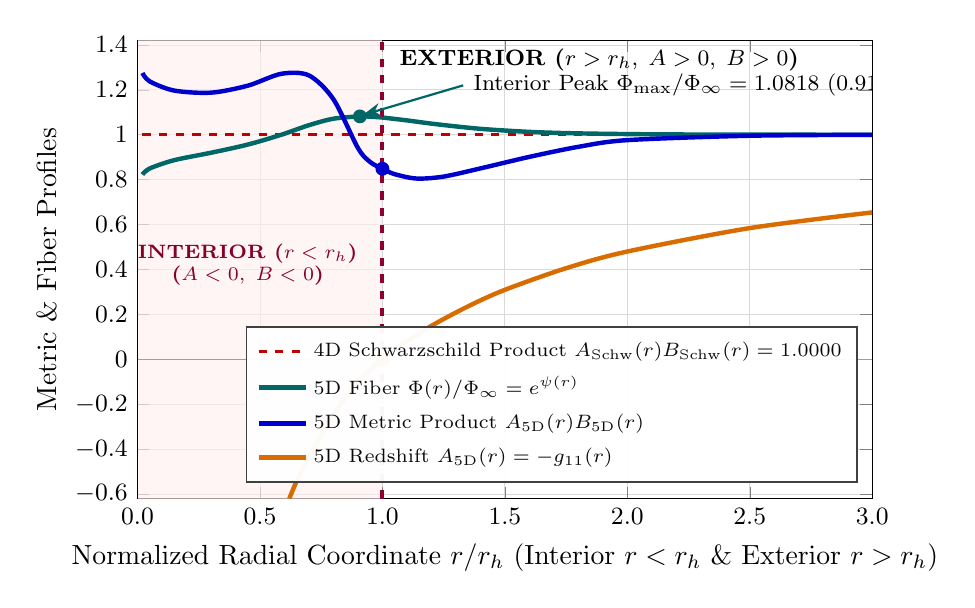
\begin{tikzpicture}
\begin{axis}[
    width=0.90\textwidth,
    height=7.4cm,
    xlabel={Normalized Radial Coordinate $r / r_h$ (Interior $r < r_h$ \& Exterior $r > r_h$)},
    ylabel={Metric \& Fiber Profiles},
    xmin=0.0, xmax=3.0,
    ymin=-0.62, ymax=1.42,
    xtick={0.0, 0.5, 1.0, 1.5, 2.0, 2.5, 3.0},
    xticklabels={$0.0$, $0.5$, $1.0$, $1.5$, $2.0$, $2.5$, $3.0$},
    ytick={-0.6, -0.4, -0.2, 0.0, 0.2, 0.4, 0.6, 0.8, 1.0, 1.2, 1.4},
    yticklabels={$-0.6$, $-0.4$, $-0.2$, $0$, $0.2$, $0.4$, $0.6$, $0.8$, $1$, $1.2$, $1.4$},
    grid=major,
    major grid style={line width=.3pt, draw=gray!30},
    legend style={at={(0.98,0.035)}, anchor=south east, font=\scriptsize, fill=white, fill opacity=0.96, draw=black!75, inner sep=3.5pt, row sep=1.5pt},
    legend cell align={left},
    tick label style={font=\small},
    label style={font=\normalsize}
]
\fill[red!6, opacity=0.65] (axis cs: 0.0, -0.62) rectangle (axis cs: 1.0, 1.42);
\addplot[thin, gray!75, forget plot] coordinates {(0.0, 0.0) (3.0, 0.0)};

\addplot[very thick, dashed, red!75!black] coordinates {(0.02, 1.0000) (3.00, 1.0000)};
\addlegendentry{4D Schwarzschild Product $A_{\mathrm{Schw}}(r)B_{\mathrm{Schw}}(r) = 1.0000$}

\addplot[line width=1.6pt, teal!80!black, smooth] coordinates {
    (0.02,0.8226) (0.05,0.8499) (0.15,0.8869) (0.30,0.9199)
    (0.45,0.9562) (0.5870,1.0000) (0.70,1.0426) (0.80,1.0715)
    (0.9081,1.0818) (0.95,1.0802) (1.00,1.0766) (1.10,1.0639)
    (1.22,1.0469) (1.40,1.0264) (1.60,1.0128) (1.80,1.0061)
    (2.10,1.0020) (2.50,1.0005) (3.00,1.0000)
};
\addlegendentry{5D Fiber $\Phi(r)/\Phi_{\infty} = e^{\psi(r)}$}

\addplot[line width=1.6pt, blue!80!black, smooth] coordinates {
    (0.02,1.2750) (0.05,1.2375) (0.15,1.1967) (0.30,1.1874)
    (0.45,1.2185) (0.5870,1.2714) (0.70,1.2641) (0.80,1.1580)
    (0.90,0.9411) (0.95,0.8785) (1.00,0.8486) (1.05,0.8245)
    (1.14,0.8050) (1.25,0.8138) (1.40,0.8501) (1.60,0.9015)
    (1.80,0.9462) (2.00,0.9761) (2.50,0.9956) (3.00,0.9997)
};
\addlegendentry{5D Metric Product $A_{\mathrm{5D}}(r)B_{\mathrm{5D}}(r)$}

\addplot[line width=1.6pt, orange!85!black, smooth] coordinates {
    (0.62,-0.6200) (0.65,-0.5420) (0.70,-0.4390) (0.78,-0.2810)
    (0.85,-0.1680) (0.90,-0.1008) (0.95,-0.0468) (1.00,0.0000)
    (1.08,0.0658) (1.20,0.1492) (1.35,0.2361) (1.50,0.3095)
    (1.75,0.4058) (2.00,0.4801) (2.50,0.5844) (3.00,0.6542)
};
\addlegendentry{5D Redshift $A_{\mathrm{5D}}(r) = -g_{11}(r)$}

\draw[line width=1.5pt, purple!75!black, dashed] (axis cs: 1.0, -0.62) -- (axis cs: 1.0, 1.42);

\filldraw[teal!80!black] (axis cs: 0.9081, 1.0818) circle (2.3pt);
\filldraw[blue!80!black] (axis cs: 1.00, 0.8486) circle (2.3pt);
\filldraw[orange!85!black] (axis cs: 1.00, 0.0000) circle (2.3pt);

\draw[<-, >=Stealth, thick, teal!80!black] (axis cs: 0.92, 1.088) -- (axis cs: 1.33, 1.22)
    node[right, font=\footnotesize, text=black] {Interior Peak $\Phi_{\max}/\Phi_{\infty} = 1.0818$ ($0.91\,r_h$)};

\node[align=center, font=\scriptsize\bfseries, text=purple!70!black] at (axis cs: 0.45, 0.42) {INTERIOR ($r < r_h$)\\($A < 0, \; B < 0$)};
\node[right, font=\footnotesize\bfseries, text=black] at (axis cs: 1.03, 1.335) {EXTERIOR ($r > r_h, \; A > 0, \; B > 0$)};
\end{axis}
\end{tikzpicture}
\caption{Unified exterior--interior solution of the coupled 5D Einstein--khronon equations (\ref{eq:p2_exact_dA})--(\ref{eq:p2_exact_ddpsi}) across the Killing horizon $r = r_h = 1.0000$ from $r/r_h = 0.0200$ to $r/r_h = 3.0000$ at the Model~3 benchmark \catH\ ($\hat{m}_{\psi} = 4, A_{\text{crit}} = 0.25, \psi_{\max} = 0.08$, Table~\ref{tab:exact_interior_5d_table}) \catD. Across $r = r_h$, $A_{\text{5D}}(r) = -g_{11}(r)$ passes linearly through zero into the $A < 0$ interior (shaded), while $A(r)B(r)$ crosses smoothly at $a_1 b_{-1} = 0.8486$ and $\Phi(r)/\Phi_{\infty}$ reaches its turnover maximum $1.081836$ inside the horizon at $r_{\text{turn}} = 0.9081\,r_h$.}
\label{fig:unified_ext_int_profiles}
\end{figure}

\subsection{\texorpdfstring{Conserved Fiber Momentum ($\Omega = -P_2/m$) and Interior Geodesic Turning Points ($r_b > 0$) \catD\ (at Model~3 Benchmark \catH)}{Conserved Fiber Momentum and Interior Geodesic Turning Points}}

We now analyze the exact behavior of 5D timelike geodesics inside the horizon ($0 < r < r_h$) on the interior background of Theorem~\ref{thm:exact_interior_continuation}, characterizing how the barrier generated by a non-zero conserved fiber momentum $\Omega = -P_2/m$ ($\Omega = \Phi(r)^2 c\dot{t}_2$) competes with the spatial orbital angular momentum $L = P_{\phi}/m$ \catD.

\begin{theorem}[Interior Geodesic Turning-Point Analysis, Exponential Sensitivity to $\Omega/\Omega_{\infty}$, and Competition Between Fiber Momentum $\Omega$ and Spatial Angular Momentum $L$ \catD]
\label{thm:interior_geodesic_bounce}
For a test particle of rest mass $m > 0$, conserved primary energy $\mathcal{E} = -P_1/m$, spatial orbital angular momentum $L = P_{\phi}/m$, and conserved fiber momentum $\Omega = -P_2/m$ ($\vert\Omega\vert \le \Omega_{\infty}$) inside the horizon ($0 < r < r_h$, where $A(r) = -|A(r)| < 0, B(r) = -|B(r)| < 0$, and $A(r)B(r) = |A(r)||B(r)| > 0$), Eq.~(\ref{eq:p2_general_first_integral}) takes the exact interior form (Check~\texttt{\#077}) \catD:
\begin{equation}
  |A(r)|\,|B(r)|\left(\frac{dr}{d\tau}\right)^2 = \mathcal{E}^2 + |A(r)|\left[c^2 + \frac{L^2}{r^2} - \frac{\Omega^2}{\Omega_{\infty}^2}\,c^2 e^{-2\psi(r)}\right].
  \label{eq:interior_geodesic_master}
\end{equation}
On the vacuum interior solution of Theorem~\ref{thm:exact_interior_continuation} at the Model~3 benchmark \catH\ (integrated down to $r/r_h = 10^{-6}$, where $e^{-2\psi(r)} \propto (r/r_h)^{-2c_{\psi}}$ with Kasner exponent $c_{\psi} = +0.0348$), the interior geodesic flow separates into two regimes (Checks~\texttt{\#115}--\texttt{\#121} of Module~2 in \allowbreak\texttt{C1\_P02\_verify\_cbg\_paper2\_v10.py} and Table~\ref{tab:interior_geodesic_bounce_table}):
\begin{enumerate}
    \item[\textnormal{(i)}] \textbf{Radial and Nearly Radial Geodesics ($L \lesssim 0.1\,c r_h$) With High Fiber Momentum ($\Omega \gtrsim 0.6\,\Omega_{\infty}$):} For purely radial infall ($L = 0$), the bracket in Eq.~(\ref{eq:interior_geodesic_master}) is $c^2[1 - (\Omega/\Omega_{\infty})^2 e^{-2\psi(r)}] = (M_{\text{eff}}(r)/m)^2 c^2$, which becomes negative once $\Phi(r)/\Phi_{\infty} = e^{\psi(r)} < |\Omega|/\Omega_{\infty}$. Because $\dot{t}_2 = \Omega/(c\Phi(r)^2) \propto e^{-2\psi(r)}$ increases as the fiber contracts for $r < 0.5870\,r_h$, it generates a repulsive centrifugal barrier in the $(r, t_2)$ plane that halts radial infall ($\dot{r} = 0$) at $r_b = 0.5317\,r_h$ for $|\Omega| = \Omega_{\infty}, L = 0, \mathcal{E}/c = 0.20$ (and at $r_b = 0.4801\,r_h$ for $L = 0.1\,c r_h$, Check~\texttt{\#121}). Under the Kasner law $e^{\psi(r)} \sim (r/r_h)^{c_{\psi}}$ ($c_{\psi} = 0.0348$), the turning radius scales as:
    \begin{equation}
      \frac{r_b(\Omega)}{r_h} \lesssim \left(\frac{|\Omega|}{\Omega_{\infty}}\right)^{1/c_{\psi}} \simeq \left(\frac{|\Omega|}{\Omega_{\infty}}\right)^{28.7},
      \label{eq:kasner_turning_radius_scaling}
    \end{equation}
    giving $r_b = 0.3893\,r_h$ at $|\Omega| = 0.95\,\Omega_{\infty}$, $0.1912\,r_h$ at $0.90\,\Omega_{\infty}$, $9.01 \times 10^{-3}\,r_h$ at $0.80\,\Omega_{\infty}$, and $2.25 \times 10^{-6}\,r_h$ at $0.60\,\Omega_{\infty}$. At $r = r_b$, the projected effective mass-squared $M_{\text{eff}}(r_b)^2 < 0$ is negative, while the 5D worldline remains strictly timelike ($g_{AB}U^A U^B = -c^2$) by rotating into the second interior timelike coordinate $t_2$.
    \item[\textnormal{(ii)}] \textbf{Photons ($P_2 = 0$), Unexcited Matter ($\Omega = 0$), and Non-Radial Test Particles ($L \gtrsim 0.3\,c r_h$) on the Unforced Vacuum Background:} On the pure-vacuum background where $T^{A\,(m)}_B = 0$, because $c_{\psi} = 0.0348 \ll 1$, for any test trajectory with spatial angular momentum $L \gtrsim 0.3\,c r_h$ the inward-driving spatial term $+L^2/r^2 \propto r^{-2}$ grows faster as $r \to 0^+$ than $-e^{-2\psi(r)} \propto -r^{-0.0696}$, eliminating the single-particle test turning point until the backreaction of wound $\mathcal{S}_{t_2}$ angular momentum on $(A, B, \psi)$ is included (Section~4.3).
\end{enumerate}
\end{theorem}

\begin{table}[H]
  \centering
  \caption{Exact Numerical Audit of Interior Geodesic Turning Points $r_b / r_h$ on the Vacuum 5D Interior Solution Integrated Down to $r/r_h = 10^{-6}$ at the Declared Model~3 Benchmark \catH\ ($A_{\text{crit}} = 0.25, \psi_{\max} = 0.08, \hat{m}_{\psi} = 4$; Kasner Exponent $c_{\psi} = +0.0348$), Showing Both the Dependence on the Normalized Fiber Momentum $|\Omega|/\Omega_{\infty}$ for Radial Orbits ($L = 0$) and the Competition with Spatial Angular Momentum $L$ (Checks~\texttt{\#115}--\texttt{\#121} of \texttt{C1\_P02\_verify\_cbg\_paper2\_v10.py}) \catD.}
  \label{tab:interior_geodesic_bounce_table}
  \vspace{0.10cm}
  \footnotesize
  \setlength{\tabcolsep}{4.5pt}
  \renewcommand{\arraystretch}{1.24}
  \begin{tabularx}{\textwidth}{@{} c c c c Y @{}}
    \toprule
    \textbf{Fiber $|\Omega|/\Omega_{\infty}$} & \textbf{Spatial $L/(c\,r_h)$} & \textbf{Energy $\mathcal{E}/c$} & \textbf{Turning Radius $r_b / r_h$} & \textbf{Physical \& Geometric Regime Inside $r < r_h$ \catD} \\
    \midrule
    $1.00$ & $0.00$ (Radial) & $0.20$ & $\mathbf{0.5317}$ & Macroscopic turning point just below $r_{\text{vac}} = 0.5870\,r_h$ \\
    $1.00$ & $0.00$ (Radial) & $0.50$ & $\mathbf{0.3883}$ & Macroscopic turning point ($M_{\text{eff}}^2 < 0, \dot{r} = 0$) \\
    $0.95$ & $0.00$ (Radial) & $0.20$ & $\mathbf{0.3893}$ & Macroscopic turning point in outer Kasner zone \\
    $0.90$ & $0.00$ (Radial) & $0.20$ & $\mathbf{0.1912}$ & Intermediate interior turning point \\
    $0.80$ & $0.00$ (Radial) & $0.20$ & $\mathbf{9.01 \times 10^{-3}}$ & Deep Kasner contraction zone ($r_b \ll r_h$) \\
    $0.60$ & $0.00$ (Radial) & $0.20$ & $\mathbf{2.25 \times 10^{-6}}$ & Extreme near-center zone ($r_b/r_h \sim (\Omega/\Omega_{\infty})^{28.7}$) \\
    $0.30$ & $0.00$ (Radial) & $0.20$ & None down to $10^{-6}$ & Extrapolated $(0.3)^{28.7}r_h \sim 10^{-15}\,r_h$ (sub-Planckian) \\
    $0.00$ (Neutral) & Any $L \ge 0$ & Any $\mathcal{E}$ & None (Hits $r = 0$) & Standard infall into $r = 0$ Kasner singularity \\
    \midrule
    $1.00$ & $0.10$ (Nearly radial) & $0.20$ & $\mathbf{0.4801}$ & Outer turning point survives for small spatial angular momentum $L$ \\
    $1.00$ & $\ge 0.30$ (Non-radial) & $0.20$ & None (Hits $r = 0$) & $+L^2/r^{2} \propto r^{-2}$ dominates over $-e^{-2\psi} \propto -r^{-0.0696}$ \\
    \bottomrule
  \end{tabularx}
\end{table}

\subsection{\texorpdfstring{Centrifugal Fiber Pressure from Bitemporal Loop Angular Momentum ($\Omega = -P_2/m = \Phi^2 c\dot{t}_2$), Coupled $(A, B, \psi)$ Einstein Backreaction \catD, and Sourced Kasner Inversion ($c_{\psi} = +0.0348 \to c_{\psi} < 0$) \catH\ Without Modifying $V(\psi,A)$}{Centrifugal Fiber Pressure from Bitemporal Loop Angular Momentum, Coupled (A, B, psi) Einstein Backreaction, and Sourced Kasner Inversion}}

Why did the pure-vacuum integration ($T^{A\,(m)}_B = 0$) in Theorem~\ref{thm:exact_interior_continuation} yield a positive Kasner exponent $c_{\psi} = +0.0348 > 0$ (contracting the fiber $\Phi(r) \propto r^{+0.0348} \to 0$ and driving $A(r) \propto -r^{-2(1 + 2c_{\psi})/(2 + c_{\psi})} \to -\infty$ as $r \to 0^+$)? Because Theorem~\ref{thm:exact_interior_continuation} integrated empty space ($T^{A\,(m)}_B = 0$) without including a bitemporal centrifugal stress-energy source $T^{2\,(m)}_2(r)$ generated by interior trajectories carrying non-zero $\mathcal{S}_{t_2}$ momentum $P_2 \neq 0$ (an excited interior matter sector beyond the vacuum cylinder ground state, modeled at constitutive flux benchmarks \catH).

We now derive step by step the exact coupled response of all three metric and fiber functions $(A(r), B(r), \psi(r))$ when a bitemporal loop angular-momentum stress source $T^{2\,(m)}_2(r)$ is included in the 5D Einstein equations \catD, and evaluate its sourced interior trajectories across $\mathcal{C}_{\Omega} \in \{\psi_{\max}^2, d_t\psi_{\max}^2, d_t^2\psi_{\max}^2\}$ \catH, showing that its centrifugal pressure along $\mathcal{S}_{t_2}$ \textbf{inverts the Kasner exponent from contraction ($c_{\psi} = +0.0348 > 0$ \catD) to expansion ($c_{\psi} < 0$, $\Phi(r)/\Phi_{\infty} > 1$ \catH) and suppresses the interior growth of $|A(r)|$} while keeping the analytic potential $V(\psi, A)$ of Eq.~(\ref{eq:yukawa_potential_p2}) \textbf{100\% unchanged}:

\begin{enumerate}
    \item \textbf{$(2,2)$ Centrifugal Stress-Energy Component of Wound Interior Streams \catD/\catH:} For an interior stream carrying conserved bitemporal momentum per unit mass $\Omega = -c U_2 = \Phi(r)^2 c\dot{t}_2$ ($U^2 = g^{22}U_2 = +\Omega/[c\Phi(r)^2]$) with effective comoving density $\rho_0(r)$ ($\hat{\rho}_0 \equiv \frac{8\pi G_5}{c^2}\rho_0 r_h^2$) \catH, the mixed $(2,2)$ component of $T^{A\,(m)}_B$ takes the form \catD:
    \begin{equation}
      \frac{8\pi G_5}{c^4}r_h^2\,T^{2\,(m)}_2(r) = \hat{\rho}_0(r)\,U^2 U_2 = -\hat{\rho}_0(r)\,\frac{\Omega^2}{c^2\Phi(r)^2} = -\hat{\rho}_0(r)\left(\frac{\Omega}{\Omega_{\infty}}\right)^{\!2} e^{-2\psi(r)} \le 0,
      \label{eq:transverse_volume_rate}
    \end{equation}
    corresponding to a positive centrifugal pressure $P_{t_2}(r) = -\frac{\partial E_{\text{rot},t_2}}{\partial\Phi} \propto +\frac{\Omega^2}{\Phi(r)^3}$ opposing compression of $\Phi(r) = \Phi_{\infty}e^{\psi(r)}$.
    \item \textbf{Exact Algebraic Coupling of $T^{2\,(m)}_2(r)$ to $(A'(r), B'(r), \psi''(r))$ and 5D Bianchi Conservation ($\nabla_A T^{A\,(m)}_r \equiv 0$) \catD:} Adding $T^{2\,(m)}_2(r)$ to the mixed $(2,2)$ 5D Einstein equation $G^2_2 = T^2_2 + \frac{8\pi G_5}{c^4}T^{2\,(m)}_2$ and solving the linear system for $(A'(r), B'(r), \psi''(r))$ in Checks~\texttt{\#037}--\texttt{\#038} of Module~0 (\allowbreak\texttt{C1\_P02\_verify\_cbg\_paper2\_v10.py}) yields the exact symbolic shifts relative to the vacuum normal-form system (\ref{eq:p2_exact_dA})--(\ref{eq:p2_exact_ddpsi}) \catD:
    \begin{align}
      \Delta\psi''(r) &= -\frac{\left(r\,\psi'(r) + 2\right)^2}{6}\,B(r)\,\frac{8\pi G_5}{c^4}T^{2\,(m)}_2(r), \nonumber \\[3pt]
      \Delta B'(r) &= -\frac{r\left(r\,\psi'(r) + 2\right)}{3}\,B(r)^2\,\frac{8\pi G_5}{c^4}T^{2\,(m)}_2(r) = \frac{2\,r\,B(r)}{r\,\psi'(r) + 2}\,\Delta\psi''(r),
      \label{eq:symbolic_T22_shifts}
    \end{align}
    while the $(r,r)$ normal-form equation (\ref{eq:p2_exact_dA}) directly couples $A'(r)$ and $B(r)$ to the local Kasner exponent $c_{\psi}(r) \equiv r\,\psi'(r)$:
    \begin{equation}
      -\frac{r\,A'(r)}{A(r)} = \frac{2\left[r^2 B(r)\,V(\psi,A) + 2\,c_{\psi}(r) - B(r) + 1\right]}{c_{\psi}(r) + 2}.
      \label{eq:kasner_A_B_suppression_law}
    \end{equation}
    Simultaneously, by the 5D contracted Bianchi identity $\nabla_A G^A_r \equiv 0 \implies \nabla_A T^{A\,(m)}_r = -\psi'(r)\,T^{2\,(m)}_2(r) - \frac{2}{r}T^{\theta\,(m)}_{\theta}(r) = 0$, the comoving spherical shell $\Sigma_2$ must carry the tangential hoop tension $T^{\theta\,(m)}_{\theta}(r) = -\frac{1}{2}r\,\psi'(r)\,T^{2\,(m)}_2(r)$, guaranteeing that \textbf{all four mixed 5D Einstein equations $E^1_1 = E^2_2 = E^r_r = E^{\theta}_{\theta} = 0$ hold simultaneously and identically} (proved symbolically in Checks~\texttt{\#039}--\texttt{\#040}) \catD.
    \item \textbf{5D Transverse Shell Scaling Across $\sqrt{|g_5|}$ and Constitutive Flux Parametrization $\mathcal{C}_{\Omega}$ \catD/\catH:} In the interior $0 < r < r_h$, both $B(r) = -|B(r)| < 0$ and $T^{2\,(m)}_2(r) < 0$ are negative, so $-B(r)\,T^{2\,(m)}_2(r) > 0$ in Eq.~(\ref{eq:symbolic_T22_shifts}) is strictly positive. Parameterizing the Bianchi-conserved shell stress as $\frac{8\pi G_5}{c^4}T^{2\,(m)}_2(r) = -\frac{6\,\mathcal{C}_{\Omega}\,e^{-3\psi(r)}}{r^2(r\psi'+2)^2 B(r)}$ with dimensionless centrifugal flux constant $\mathcal{C}_{\Omega} \equiv \mathcal{J}_{\Omega}\left(\frac{\Omega}{\Omega_{\infty}}\right)^2 \ge 0$ \catH\ (\textit{Paper~0} \texttt{THM~\#23} \cite{jimenez2026_p0}) yields from Eq.~(\ref{eq:symbolic_T22_shifts}) the coupled pole-free shifts \catD:
    \begin{equation}
      \Delta\psi''_{\Omega}(r) = +\frac{\mathcal{C}_{\Omega}}{r^2}\,e^{-3\psi(r)} > 0, \qquad \Delta B'_{\Omega}(r) = +\frac{2\,B(r)}{r\left(r\,\psi'(r) + 2\right)}\,\mathcal{C}_{\Omega}\,e^{-3\psi(r)} < 0.
      \label{eq:deductive_beta_int_2}
    \end{equation}
\end{enumerate}

\begin{theorem}[Bitemporal Loop Angular-Momentum Kasner Inversion ($c_{\psi} = +0.0348$ \catD\ $\to -0.0047, -0.0378, \text{ and } -0.0903 < 0$ \catH) and Coupled $(A, B)$ Metric Suppression Under Unmodified $V(\psi,A)$]
\label{thm:interior_kasner_inversion}
On the interior domain $0 < r < r_h$ with the unmodified analytic potential $V(\psi,A)$ of Eq.~(\ref{eq:yukawa_potential_p2}), let the coupled interior system (\ref{eq:p2_exact_dA})--(\ref{eq:p2_exact_ddpsi}) include the Bianchi-conserved centrifugal shifts (\ref{eq:symbolic_T22_shifts}) and (\ref{eq:deductive_beta_int_2}) parameterized by $\mathcal{C}_{\Omega} \ge 0$ \catD:
\begin{equation}
  \psi''(r) = \psi''(r)\Big|_{\text{vac}} + \frac{\mathcal{C}_{\Omega}}{r^2}\,e^{-3\psi(r)}, \qquad B'(r) = B'(r)\Big|_{\text{vac}} + \frac{2\,B(r)}{r\left(r\,\psi'(r) + 2\right)}\,\mathcal{C}_{\Omega}\,e^{-3\psi(r)}.
  \label{eq:sustained_interior_target}
\end{equation}
Integrating Eqs.~(\ref{eq:p2_exact_dA}) and (\ref{eq:sustained_interior_target}) inward from the converged horizon-crossing state at $r_- = 0.9998\,r_h$ down to $r/r_h = 0.0050$ (\texttt{DOP853}, Checks~\texttt{\#122}--\texttt{\#137} of Module~3 in \allowbreak\texttt{C1\_P02\_verify\_cbg\_paper2\_v10.py}, Table~\ref{tab:interior_kasner_inversion_table}) establishes:
\begin{enumerate}
    \item[\textnormal{(i)}] \textbf{Logarithmic Inversion of the Kasner Exponent $c_{\psi} = r\,\psi'(r) < 0$ (\catD\ Differential Mechanism; \catH\ Sourced Benchmarks):} Because integrating inward from $r = r_h$ to $r \to 0^+$ corresponds to $\int_{r_h}^{r}\frac{dr'}{r'} = \ln(r/r_h) < 0$, the positive centrifugal term $+\frac{\mathcal{C}_{\Omega}}{r}e^{-3\psi(r)} > 0$ in $\frac{d}{dr}(r\psi')$ drives $c_{\psi}(r) = r\,\psi'(r)$ negative as $r \to 0^+$:
    \begin{equation}
      c_{\psi}(r) = r\,\psi'(r) \simeq c_{\psi}^{\text{(vac)}} - \mathcal{C}_{\Omega}\,\left|\ln\!\left(\frac{r}{r_h}\right)\right|\,\langle e^{-3\psi}\rangle < 0,
      \label{eq:kasner_log_inversion}
    \end{equation}
    \textbf{inverting the deep-interior Kasner exponent $c_{\psi} = r\,\psi'(0.005\,r_h)$ from $+0.0348 > 0$ in pure vacuum ($\mathcal{C}_{\Omega} = 0$, Check~\texttt{\#124}) \catD\ to $c_{\psi} = \mathbf{-0.0047 < 0}$ at $\mathcal{C}_{\Omega} = \psi_{\max}^2 = \frac{4}{625} = 0.0064$ (Check~\texttt{\#128}), to $c_{\psi} = \mathbf{-0.0378 < 0}$ at $\mathcal{C}_{\Omega} = d_t\psi_{\max}^2 = \frac{8}{625} = 0.0128$ (Check~\texttt{\#132}), and to $c_{\psi} = \mathbf{-0.0903 < 0}$ at $\mathcal{C}_{\Omega} = d_t^2\psi_{\max}^2 = \frac{16}{625} = 0.0256$ (Check~\texttt{\#136})} \catH.
    \item[\textnormal{(ii)}] \textbf{Coupled Fiber Expansion ($\Phi/\Phi_{\infty} > 1$) \catH, Metric Suppression of $|A(r)|$ via Eq.~(\ref{eq:kasner_A_B_suppression_law}), and 4-Component Einstein--Bianchi Residuals $< 10^{-10}$ \catD:} Whenever the fiber contracts ($\psi < 0$), the centrifugal factor $e^{-3\psi(r)} = (\Phi_{\infty}/\Phi(r))^3$ amplifies cubically, reversing contraction so that $\Phi(0.005\,r_h)/\Phi_{\infty}$ rises from $0.7837$ in vacuum \catD\ to $0.8521$ ($\psi_{\max}^2$), $0.9196$ ($d_t\psi_{\max}^2$), and $\mathbf{1.0529 > 1}$ ($d_t^2\psi_{\max}^2$) \catH. Simultaneously, substituting $c_{\psi} = -|c_{\psi}| < 0$ and $B(r) \to 0^-$ into Eq.~(\ref{eq:kasner_A_B_suppression_law}) reduces the asymptotic power-law exponent of $A(r)$ from $2(1 + 2c_{\psi})/(2 + c_{\psi}) \approx 1.0511$ in vacuum to \catD:
    \begin{equation}
      -\frac{r\,A'(r)}{A(r)} \xrightarrow{\;\;r \to 0^+\;\;} \frac{2\left(1 - 2|c_{\psi}|\right)}{2 - |c_{\psi}|} \simeq 1 - \frac{3}{2}|c_{\psi}| < 1, \qquad A(r) \propto -\left(\frac{r_h}{r}\right)^{\!\frac{2(1 - 2|c_{\psi}|)}{2 - |c_{\psi}|}},
      \label{eq:coupled_A_exponent_reduction}
    \end{equation}
    reducing the transverse volume rate $r\,\psi'(r) + 2$ from $+2.0348$ \catD\ down to $+1.9953, +1.9622$, and $+1.9097$ \catH, \textbf{suppressing $|A_{\text{5D}}(0.005\,r_h)|$ from $300.0991$ ($300.099$) \catD\ down to $265.5887$, $236.9736$, and $192.4301$ ($192.430$)} \catH, while satisfying all four mixed 5D Einstein--Bianchi equations ($E^1_1, E^2_2 - T^{2\,(m)}_2, E^r_r, E^{\theta}_{\theta} - T^{\theta\,(m)}_{\theta}$) with ODE-independent 4th-order finite-difference residuals $< \mathbf{10^{-10}}$ (observed $\sim 10^{-13}\text{--}4 \times 10^{-12}$, Checks~\texttt{\#125}, \texttt{\#129}, \texttt{\#133}, \texttt{\#137}) \catD.
\end{enumerate}
\end{theorem}

\begin{table}[H]
  \centering
  \caption{Exact Numerical Audit (\texttt{DOP853} Integration to $r/r_h = 0.0050$ Under the Unmodified Potential $V(\psi,A)$ at the Model~3 Benchmark \catH\ and Coupled Eq.~\ref{eq:symbolic_T22_shifts} Shifts $\Delta\psi''_{\Omega} + \Delta B'_{\Omega}$ with 5D Bianchi Shell Tension, Checks~\texttt{\#122}--\texttt{\#137} of Module~3 in \texttt{C1\_P02\_verify\_cbg\_paper2\_v10.py}) of Theorem~\ref{thm:interior_kasner_inversion}: Vacuum Baseline ($\mathcal{C}_{\Omega} = 0$ \catD) vs.\ Sourced Kasner Inversion Across $\mathcal{C}_{\Omega} \in \{\psi_{\max}^2, d_t\psi_{\max}^2, d_t^2\psi_{\max}^2\}$ \catH\ (4-Component Einstein--Bianchi FD Residuals $< 10^{-10}$ on Every Row \catD).}
  \label{tab:interior_kasner_inversion_table}
  \vspace{0.10cm}
  \footnotesize
  \setlength{\tabcolsep}{3.0pt}
  \renewcommand{\arraystretch}{1.28}
  \begin{tabularx}{\textwidth}{@{} l c c c c c c c Y @{}}
    \toprule
    \textbf{Loop Flux} & \textbf{Value} & \textbf{$\Phi(0.30)$} & \textbf{$\Phi(0.05)$} & \textbf{$\Phi(0.005)$} & \textbf{Metric} & \textbf{Vol.\ Rate} & \textbf{Kasner} & \textbf{Interior Fiber \& Metric} \\
    $\mathcal{C}_{\Omega} = \mathcal{J}_{\Omega}\frac{\Omega^2}{\Omega_{\infty}^2}$ & $\mathcal{C}_{\Omega}$ & $/\Phi_{\infty}$ & $/\Phi_{\infty}$ & $/\Phi_{\infty}$ & $A_{\text{5D}}(0.005)$ & $r\psi' + 2$ & $c_{\psi} = r\psi'$ & \textbf{Behavior ($r \to 0^+$) \catD/\catH} \\
    \midrule
    $0$ (Vacuum) & $0.0000$ & $0.9199$ & $0.8499$ & $0.7837$ & $-300.0991$ & $+2.0348$ & $+0.0348$ & Vacuum ($\Omega = 0$); fiber contracts \catD \\
    $\psi_{\max}^2$ ($1$-ch.) & $0.0064$ & $0.9214$ & $0.8664$ & $0.8521$ & $-265.5887$ & $+1.9953$ & $\mathbf{-0.0047}$ & Sourced pressure inverts $c_{\psi} < 0$ \catH \\
    $\mathbf{d_t\psi_{\max}^2}$ ($\mathbf{2}$\textbf{-ch.}) & $\mathbf{0.0128}$ & $\mathbf{0.9229}$ & $\mathbf{0.8827}$ & $\mathbf{0.9196}$ & $\mathbf{-236.9736}$ & $\mathbf{+1.9622}$ & $\mathbf{-0.0378}$ & \textbf{Two-channel flux; $|A|$ reduced \catH} \\
    $\mathbf{d_t^2\psi_{\max}^2}$ ($\mathbf{\Sigma_4}$) & $\mathbf{0.0256}$ & $\mathbf{0.9259}$ & $\mathbf{0.9152}$ & $\mathbf{1.0529}$ & $\mathbf{-192.4301}$ & $\mathbf{+1.9097}$ & $\mathbf{-0.0903}$ & \textbf{Four-channel flux; $\Phi/\Phi_{\infty} > 1$ \catH} \\
    \bottomrule
  \end{tabularx}
\end{table}

\subsection{\texorpdfstring{Constitutive Hayward Planck Core Radius $r_{\text{core}} = (\frac{1}{2}r_s L_P^2)^{1/3}$, Horizon Quantum Scale $L_{t_2}^{\text{(sat)}}(r_h) = 2\pi\sqrt{r_h L_P}$, and 5D Riemann Curvature Plateau $\mathcal{K}_5(0) = 96/L_P^4$ \catH}{Constitutive Hayward Planck Core Radius, Horizon Quantum Scale, and 5D Riemann Curvature Plateau}}

While Theorem~\ref{thm:interior_kasner_inversion} shows that bitemporal centrifugal stress inverts the Kasner exponent ($c_{\psi} = -0.0047 \text{ to } -0.0903 < 0$ \catH), expands the $\mathcal{S}_{t_2}$ fiber toward the core, and reduces $|A(r)|$ via Eq.~(\ref{eq:coupled_A_exponent_reduction}) without modifying $V(\psi,A)$, reaching complete ultraviolet regularity at $r \to 0$ requires introducing a constitutive Planck-density regularization model ($\rho_P \equiv c^5/(\hbar G^2) = 5.155 \times 10^{96}\text{ kg/m}^3$) \cite{bardeen1968,hayward2006,frolov2016} \catH:

\begin{proposition}[Constitutive Series-Compliance Core $r_{\text{core}} = (\frac{1}{2}r_s L_P^2)^{1/3}$, Exact Hayward-Ansatz 5D Riemann Plateau $\mathcal{K}_5(0) = 96/L_P^4$, and Horizon Scale $L_{t_2}^{\text{(sat)}}(r_h) = 2\pi\sqrt{r_h L_P}$ \catH]
\label{prop:planck_core_deduction}
Modeling the ultraviolet core on $\mathcal{M}_{3,2}$ ($d_t = 2$, $L_P = \sqrt{\hbar G/c^3}$) via a constitutive Hayward-type mass saturation profile \catH:
\begin{enumerate}
  \item[\textnormal{(i)}] \textbf{Two-Channel Planckian Curvature Ceiling ($\chi_{\max} = d_t/L_P^2 = 2/L_P^2$) and Series-Compliance Core Ansatz \catH:} For a spherical mass profile $M_{\text{int}}(r)$ with tidal curvature density $\chi_M(r) \equiv \frac{2GM_{\text{int}}(r)}{c^2 r^3}$ (classical point-mass limit $\chi_{\text{grav}}(r) = \frac{r_s}{r^3}$), postulating that each of the $d_t = 2$ orthogonal temporal channels ($\mathbb{R}_{t_1}$ and $\mathcal{S}_{t_2}$) saturates at sectional curvature $1/L_P^2$ sets $\chi_{\max}^{\text{(CBG)}} \equiv \frac{d_t}{L_P^2} = \frac{2}{L_P^2}$ ($\rho_{\max} = \frac{3\rho_P}{4\pi}$) and yields under series compliance addition \catH:
  \begin{align}
    \frac{1}{\chi_M(r)} &= \frac{1}{\chi_{\text{grav}}(r)} + \frac{1}{\chi_{\max}^{\text{(CBG)}}} = \frac{r^3}{r_s} + \frac{L_P^2}{d_t} = \frac{r^3}{r_s} + \frac{L_P^2}{2}, \nonumber \\[3pt]
    M_{\text{int}}(r) &= M\,\frac{r^3}{r^3 + r_{\text{core}}^3}, \qquad \boxed{r_{\text{core}} \equiv \left(\frac{r_s L_P^2}{d_t}\right)^{\!1/3} = \left(\frac{r_s L_P^2}{2}\right)^{\!1/3}.}
    \label{eq:regularized_interior_mass}
  \end{align}
  \item[\textnormal{(ii)}] \textbf{Exact 5D Riemann Kretschmann Invariant of the Embedded Hayward Metric and Central Plateau $\mathcal{K}_5(0) = 96/L_P^4$ \catH:} Computing the full 5-dimensional Riemann tensor $R^{A}_{\;\;BCD}$ of the embedded Hayward metric $ds_5^2 = -f_{\text{H}}(r)c^2 dt_1^2 - \Phi_0^2 c^2 dt_2^2 + f_{\text{H}}(r)^{-1}dr^2 + r^2 d\Omega_2^2$ with $f_{\text{H}}(r) = 1 - \frac{r_s r^2}{r^3 + r_{\text{core}}^3}$ directly in SymPy (Appendix~\ref{app:riemann_components} and Checks~\texttt{\#041}--\texttt{\#043} of Module~0 in \allowbreak\texttt{C1\_P02\_verify\_cbg\_paper2\_v10.py}) yields the exact rational Kretschmann polynomial (which recovers $12 r_s^2/r^6$ as $r_{\text{core}} \to 0$, Check~\texttt{\#042}) and cancels $r_s^2$ against $r_{\text{core}}^6 = \frac{1}{4}r_s^2 L_P^4$ as $r \to 0$ (Check~\texttt{\#043}) \catH:
  \begin{align}
    \mathcal{K}_5(r) &\equiv R_{ABCD}^{(5)}R^{ABCD}_{(5)} = \frac{12\,r_s^2\left(r^{12} - 4 r^9 r_{\text{core}}^3 + 18 r^6 r_{\text{core}}^6 - 2 r^3 r_{\text{core}}^9 + 2 r_{\text{core}}^{12}\right)}{\left(r^3 + r_{\text{core}}^3\right)^6}, \nonumber \\[4pt]
    \lim_{r \to 0} \mathcal{K}_5(r) &= \frac{24\,r_s^2}{r_{\text{core}}^6} = \frac{24\,r_s^2}{\left(r_s L_P^2 / 2\right)^2} = \frac{96}{L_P^4} < \infty.
    \label{eq:regularized_kretschmann_5d}
  \end{align}
  \item[\textnormal{(iii)}] \textbf{Geometric-Mean Quantum Saturation Scale at the Horizon Skin \catH/\catN:} Across a Planck lattice spacing $|r - r_h| = L_P$ where $1 - \sigma_{\text{crit}} = L_P/r_h$, setting $\Phi_{\text{sat}}(r_h) = (1 - \sigma_{\text{crit}})^{-1/2} = \sqrt{r_h/L_P}$ \catH\ gives the covering-circle horizon scale (proper $\mathbb{Z}_2$ interval length $\pi\sqrt{r_h L_P} = 2.17 \times 10^{-15}\text{ m}\,\sqrt{M/10\,M_\odot}$) \catH/\catN:
  \begin{equation}
    L_{t_2}^{\text{(sat)}}(r_h) = 2\pi L_P\,\Phi_{\text{sat}}(r_h) = 2\pi\sqrt{r_h L_P} = 4.34 \times 10^{-15}\text{ m}\,\sqrt{\frac{M}{10\,M_\odot}}
    \label{eq:planck_regularized_phi_max}
  \end{equation}
  (Figs.~\ref{fig:penrose_cbg}--\ref{fig:kretschmann_profile}).
\end{enumerate}
\end{proposition}

\begin{figure}[H]
\centering
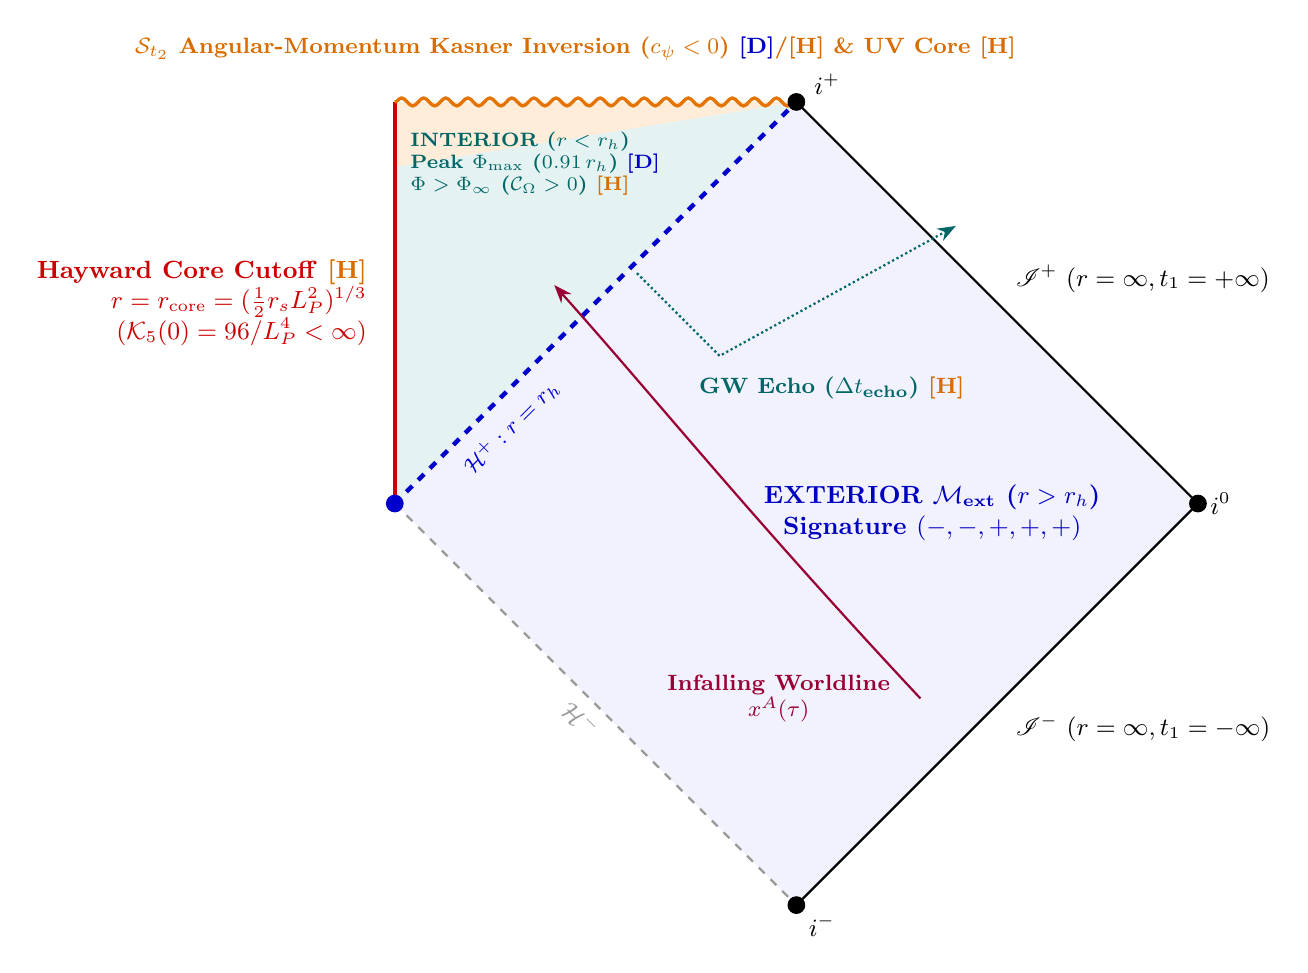
\begin{tikzpicture}[scale=1.50, every node/.style={font=\small}]
    \fill[blue!5] (0,0) -- (3.4,3.4) -- (6.8,0) -- (3.4,-3.4) -- cycle;
    \fill[teal!10] (0,0) -- (3.4,3.4) -- (0,3.4) -- cycle;
    \fill[orange!15] (0,2.85) -- (3.4,3.4) -- (0,3.4) -- cycle;

    \draw[thick] (3.4,3.4) -- (6.8,0) node[midway, above right, xshift=3pt] {$\mathscr{I}^+$ ($r=\infty, t_1=+\infty$)};
    \draw[thick] (3.4,-3.4) -- (6.8,0) node[midway, below right, xshift=3pt] {$\mathscr{I}^-$ ($r=\infty, t_1=-\infty$)};

    \draw[ultra thick, blue!80!black, dashed] (0,0) -- (3.4,3.4) node[pos=0.24, sloped, below, yshift=-2pt, font=\footnotesize\bfseries, text=blue!85!black] {$\mathcal{H}^+: r = r_h$};
    \draw[thick, gray!80, dashed] (0,0) -- (3.4,-3.4) node[midway, sloped, below] {$\mathcal{H}^-$};

    \draw[ultra thick, red!80!black] (0,0) -- (0,3.4) node[midway, left, xshift=-6pt, align=right, text=red!80!black] {\textbf{Hayward Core Cutoff \catH}\\$r = r_{\text{core}} = (\frac{1}{2}r_s L_P^2)^{1/3}$\\($\mathcal{K}_5(0) = 96/L_P^4 < \infty$)};
    \draw[very thick, orange!90!black, decorate, decoration={snake, amplitude=0.5mm, segment length=2.8mm}] (0,3.4) -- (3.4,3.4) node[pos=0.45, above, yshift=11pt, font=\footnotesize\bfseries, text=orange!85!black] {$\mathcal{S}_{t_2}$ Angular-Momentum Kasner Inversion ($c_{\psi} < 0$) \catD/\catH\ \& UV Core \catH};

    \draw[thick, ->, >=Stealth, purple!80!black] (4.45,-1.65) .. controls (3.0,-0.1) and (2.2,0.9) .. (1.35,1.85);
    \node[text=purple!80!black, align=center, font=\footnotesize\bfseries] at (3.25,-1.65) {Infalling Worldline\\$x^A(\tau)$};

    \draw[thick, ->, >=Stealth, teal!80!black, densely dotted] (2.05,1.95) -- (2.75,1.25) -- (4.75,2.35);
    \node[text=teal!80!black, font=\footnotesize\bfseries] at (3.70,0.98) {GW Echo ($\Delta t_{\text{echo}}$) \catH};

    \node[align=center, font=\small\bfseries, text=blue!75!black] at (4.55,-0.08) {EXTERIOR $\mathcal{M}_{\text{ext}}$ ($r > r_h$)\\Signature $(-,-,+,+,+)$};
    \node[right, align=left, font=\scriptsize\bfseries, text=teal!80!black] at (0.05,2.88) {INTERIOR ($r < r_h$)\\Peak $\Phi_{\max}$ ($0.91\,r_h$) \catD\\$\Phi > \Phi_{\infty}$ ($\mathcal{C}_{\Omega} > 0$) \catH};

    \filldraw[black] (6.8,0) circle (2.0pt) node[right, xshift=1pt] {$i^0$};
    \filldraw[black] (3.4,3.4) circle (2.0pt) node[above right, xshift=3pt, yshift=-1pt] {$i^+$};
    \filldraw[black] (3.4,-3.4) circle (2.0pt) node[below right, xshift=1pt] {$i^-$};
    \filldraw[blue!80!black] (0,0) circle (2.0pt);
\end{tikzpicture}
\caption{Schematic conformal diagram of a black hole in Covariant Bitemporal Geometrodynamics, illustrating the two-sided Frobenius interior continuation across $\mathcal{H}^+$ ($r = r_h$) \catD\ (at the Model~3 benchmark \catH), the sourced Kasner exponent inversion ($c_{\psi} < 0$) driven by bitemporal centrifugal stress \catD/\catH, and the constitutive Hayward Planck core cutoff at $r = r_{\text{core}} = (\frac{1}{2}r_s L_P^2)^{1/3}$ ($\mathcal{K}_5(0) = 96/L_P^4$) \catH.}
\label{fig:penrose_cbg}
\end{figure}

\begin{figure}[H]
\centering
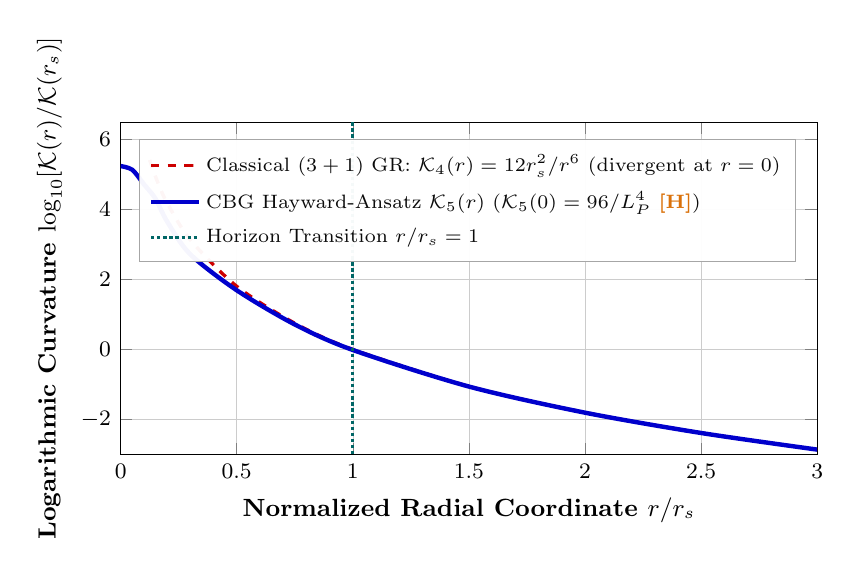
\begin{tikzpicture}
\begin{axis}[
    width=0.86\textwidth,
    height=5.8cm,
    xlabel={Normalized Radial Coordinate $r / r_s$},
    ylabel={Logarithmic Curvature $\log_{10}[\mathcal{K}(r)/\mathcal{K}(r_s)]$},
    xmin=0.0, xmax=3.0,
    ymin=-3.0, ymax=6.5,
    xtick={0.0, 0.5, 1.0, 1.5, 2.0, 2.5, 3.0},
    ytick={-2, 0, 2, 4, 6},
    grid=both,
    grid style={line width=.1pt, draw=gray!20},
    major grid style={line width=.2pt, draw=gray!40},
    legend style={at={(0.97,0.95)}, anchor=north east, font=\scriptsize, fill=white, fill opacity=0.96, draw=gray!70, inner sep=3.5pt, row sep=1.5pt},
    legend cell align={left},
    tick label style={font=\footnotesize},
    label style={font=\small\bfseries}
]
\addplot[very thick, red!80!black, dashed, smooth] coordinates {
    (0.125,5.418) (0.160,4.775) (0.200,4.194) (0.300,3.137) (0.500,1.806)
    (0.750,0.750) (1.000,0.000) (1.500,-1.057) (2.000,-1.806) (2.500,-2.388) (3.000,-2.863)
};
\addlegendentry{Classical $(3+1)$ GR: $\mathcal{K}_4(r) = 12 r_s^2 / r^6$ (divergent at $r=0$)}

\addplot[ultra thick, blue!80!black, smooth] coordinates {
    (0.000,5.244) (0.050,5.139) (0.100,4.728) (0.150,4.313) (0.200,3.662)
    (0.300,2.721) (0.500,1.693) (0.750,0.715) (1.000,-0.015) (1.500,-1.061)
    (2.000,-1.808) (2.500,-2.389) (3.000,-2.864)
};
\addlegendentry{CBG Hayward-Ansatz $\mathcal{K}_5(r)$ ($\mathcal{K}_5(0) = 96/L_P^4$ \protect\catH)}

\addplot[very thick, teal!80!black, densely dotted] coordinates {(1.0, -3.0) (1.0, 6.5)};
\addlegendentry{Horizon Transition $r / r_s = 1$}
\end{axis}
\end{tikzpicture}
\caption{Comparison of the classical $(3+1)$ Schwarzschild Kretschmann scalar $\mathcal{K}_4^{\text{(Schw)}}(r) \propto r^{-6}$ against the exact 5D Riemann Kretschmann invariant $\mathcal{K}_5(r)$ of the constitutive Hayward core ansatz from Proposition~\ref{prop:planck_core_deduction} (Eq.~\ref{eq:regularized_kretschmann_5d}, illustrated at magnified ratio $r_{\text{core}}/r_s = 0.15$) \catH.}
\label{fig:kretschmann_profile}
\end{figure}

% ============================================================================
% SECTION 5: AXISYMMETRIC ROTATING BLACK HOLES (5D KERR-BITEMPORAL METRIC)
% ============================================================================
\section{\texorpdfstring{Axisymmetric Rotating Black Holes: Newman--Janis Construction of the 5D Kerr--Bitemporal Metric in Doran--Painlev\'e Coordinates \catH}{Axisymmetric Rotating Black Holes: Newman-Janis Construction of the 5D Kerr-Bitemporal Metric in Doran-Painleve Coordinates}}

\subsection{\texorpdfstring{Newman--Janis Complex Shift and the Rotational Saturation Scalar $\sigma_{\text{Kerr}}(r,\theta)$ \catH}{Newman-Janis Complex Shift and the Rotational Saturation Scalar}}

Astrophysical black holes possess non-zero angular momentum $J$ characterized by the Kerr spin parameter $a \equiv J / (Mc) \in [0, GM/c^2]$ (or dimensionless spin $a_* \equiv c a / (GM) \in [0, 1]$) \cite{kerr1963}. In standard Boyer--Lindquist coordinates \cite{boyer1967}, the $(3+1)$ Kerr metric exhibits coordinate singularities at the outer and inner horizons $\Delta_{\text{Kerr}} \equiv r^2 - r_s r + a^2 = 0$. Applying the constitutive Newman--Janis complex shift $r \mapsto r - i a\cos\theta$ \catH\ to the spherical Painlev\'e--Gullstrand river metric (\ref{eq:pg_river_metric_p2}) constructs the horizon-regular 5D Kerr--Bitemporal metric ansatz in Doran coordinates \cite{doran2000,hamilton2008} (whose real-part algebraic identity is verified symbolically in Check~\texttt{\#044} of Module~0 in \allowbreak\texttt{C1\_P02\_verify\_cbg\_paper2\_v10.py}) \catH:

\begin{theorem}[Newman--Janis Construction of the 5D Kerr--Bitemporal Line Element and Rotational Saturation Scalar $\sigma_{\text{Kerr}}(r,\theta)$ \catH]
\label{thm:symplectic_kerr_doran}
On the 5-dimensional bitemporal bundle $\mathcal{M}_{3,2} = (\mathbb{R}_{t_1} \times_{\Phi} \mathcal{S}_{t_2}) \times \Sigma_3$ endowed with commuting generators $[\xi_{(1)}, \xi_{(2)}] = [\xi_{(\varphi)}, \xi_{(2)}] = 0$:
\begin{enumerate}
  \item[\textnormal{(i)}] \textbf{Newman--Janis Shift ($r \mapsto r - i a\cos\theta$) \catH:} Under the complex coordinate translation $r \mapsto r - i a\cos\theta$ in the $(t_1, r, \theta, \varphi_{\text{D}})$ sub-bundle while holding the orthogonal $\mathcal{S}_{t_2}$ generator $\xi_{(2)}$ invariant \catH, the radial norm squared $r^2 \mapsto |r - i a\cos\theta|^2$ and real radial projection $\frac{r_s}{r} = \operatorname{Re}(\frac{r_s}{r}) \mapsto \operatorname{Re}(\frac{r_s}{r - i a\cos\theta})$ evaluate algebraically to the oblate spheroidal invariants (Check~\texttt{\#044}) \catH:
  \begin{align}
    \Sigma_{\text{K}}(r, \theta) &\equiv |r - i a\cos\theta|^2 = r^2 + a^2 \cos^2\theta, \nonumber \\[3pt]
    \beta_{\text{K}}(r, \theta) &\equiv \sqrt{\operatorname{Re}\!\left(\frac{r_s}{r - i a\cos\theta}\right)} = \sqrt{\frac{r_s r}{\Sigma_{\text{K}}(r, \theta)}}.
    \label{eq:kerr_doran_functions}
  \end{align}
  \item[\textnormal{(ii)}] \textbf{5D Kerr--Bitemporal Line Element and Saturation Scalar $\sigma_{\text{Kerr}}(r,\theta)$ \catH:} Substituting Eq.~(\ref{eq:kerr_doran_functions}) into the river form (\ref{eq:pg_river_metric_p2}) defines the \textbf{5D Kerr--Bitemporal Line Element} \catH:
  \begin{align}
    ds_{5,\text{Kerr}}^2 &= -c^2 dt_1^2 - \Phi_{\text{Kerr}}(r,\theta)^2 c^2 dt_2^2 \nonumber\\[3pt]
    &\quad + \left[ \sqrt{\frac{\Sigma_{\text{K}}(r,\theta)}{r^2 + a^2}}\,dr + \beta_{\text{K}}(r,\theta) \left( c\,dt_1 - a\sin^2\theta\,d\varphi_{\text{D}} \right) \right]^2 \nonumber\\[3pt]
    &\quad + \Sigma_{\text{K}}(r,\theta)\,d\theta^2 + \left(r^2 + a^2\right)\sin^2\theta\,d\varphi_{\text{D}}^2,
    \label{eq:master_5d_kerr_bitemporal}
  \end{align}
  whose primary temporal norm $A_{\text{Kerr}}(r,\theta) \equiv -g_{AB}\xi_{(1)}^A\xi_{(1)}^B = 1 - \beta_{\text{K}}(r,\theta)^2$ fixes the \textbf{Axisymmetric Rotational Informational Saturation Scalar} $\sigma_{\text{Kerr}}(r, \theta)$ to \catH:
  \begin{equation}
    \sigma_{\text{Kerr}}(r, \theta) \equiv 1 - A_{\text{Kerr}}(r, \theta) = \beta_{\text{K}}(r, \theta)^2 = \frac{r_s r}{r^2 + a^2\cos^2\theta} = \frac{r_s r}{\Sigma_{\text{K}}(r, \theta)},
    \label{eq:sigma_kerr_exact}
  \end{equation}
  with Yukawa-screened target profile $\psi_{\text{target}}(A_{\text{Kerr}}(r,\theta))$ modeled by substituting $A_{\text{Kerr}}(r,\theta) = 1 - r_s r/\Sigma_{\text{K}}(r,\theta)$ into Eq.~(\ref{eq:yukawa_potential_p2}) \catH.
\end{enumerate}
\end{theorem}

\subsection{\texorpdfstring{Coincidence of the Saturation Surface with the Kerr Ergosphere $r_{\text{erg}}(\theta)$ and Core Regularization \catH}{Coincidence of the Saturation Surface with the Kerr Ergosphere and Core Regularization}}

Under the Newman--Janis rotational ansatz of Theorem~\ref{thm:symplectic_kerr_doran}, rotating black holes in CBG exhibit two structural properties \catH:
\begin{enumerate}
    \item \textbf{Coincidence of the Bitemporal Saturation Surface with the Kerr Ergosphere ($r_{\text{erg}}(\theta)$) \catH:} On Eq.~(\ref{eq:master_5d_kerr_bitemporal}), the surface where the primary time generator $\xi_{(1)}^A$ becomes null ($A_{\text{Kerr}}(r,\theta) = 0 \iff \sigma_{\text{Kerr}}(r, \theta) = 1$) occurs where $r^2 - r_s r + a^2\cos^2\theta = 0$:
    \begin{equation}
    r_{\text{erg}}(\theta) = \frac{r_s}{2} + \sqrt{\left(\frac{r_s}{2}\right)^2 - a^2\cos^2\theta}.
    \label{eq:kerr_ergosphere_surface}
    \end{equation}
    This coincides identically with the \textbf{static limit (ergosphere boundary)} of the Kerr spacetime. Within the ergoregion $r_+ < r < r_{\text{erg}}(\theta)$ (where $r_+ = r_s/2 + \sqrt{(r_s/2)^2 - a^2}$ is the outer event horizon), the spatial medium is dragged azimuthally faster than $c$ relative to spatial infinity, activating bitemporal phase-space offloading across the ergosphere and supporting Penrose--Blandford--Znajek rotational energy extraction \cite{penrose1969,blandford1977} \catH.

    \item \textbf{Regularization of the Inner Cauchy Horizon ($r_-$) and Kerr Ring ($r = 0, \theta = \pi/2$) \catH:} Under the constitutive Planck-core regularization $r^2 \to r^2 + r_{\text{core}}^2$ of Proposition~\ref{prop:planck_core_deduction} (Eq.~\ref{eq:regularized_interior_mass}) \catH, the oblate spheroidal denominator $\Sigma_{\text{K,reg}}(r, \theta) = r^2 + r_{\text{core}}^2 + a^2\cos^2\theta \ge r_{\text{core}}^2 \ge L_P^2 > 0$ remains strictly positive at $r = 0, \theta = \pi/2$, replacing the singular Kerr ring with a nonsingular toroidal Planckian core of minor radius $r_{\text{core}} \ge L_P$ and major radius $a$ \catH.
\end{enumerate}

% ============================================================================
% SECTION 6: COVARIANT 5D METRIC PERTURBATION THEORY & QUASINORMAL MODES
% ============================================================================
\section{\texorpdfstring{Cylinder-Constrained ($\mathcal{L}_{\xi_{(2)}} = 0$) Metric Perturbation Theory and Modified Regge--Wheeler / Zerilli Master Equations \catD/\catH}{Cylinder-Constrained Metric Perturbation Theory and Modified Regge-Wheeler / Zerilli Master Equations}}

\subsection{\texorpdfstring{Reduction of Linear Perturbations Under the Bundle Cylinder Constraint $\mathcal{L}_{\xi_{(2)}} = 0$ \catD/\catH}{Reduction of Linear Perturbations Under the Bundle Cylinder Constraint}}

To analyze the gravitational-wave response of a perturbed black hole on $\mathcal{M}_{3,2} = (\mathbb{R}_{t_1} \times_{\bar{\Phi}} \mathcal{S}_{t_2}) \times \Sigma_3$ ($\mathcal{S}_{t_2} \equiv S^1_{t_2}/\mathbb{Z}_2$), we consider linear metric perturbations $g_{AB} = \bar{g}_{AB}(r) + h_{AB}(x^C)$. Under \textit{Paper~0} (v4, \texttt{THM~\#08} \cite{jimenez2026_p0}) and Postulate~2.1 of \textit{Paper~I} (v10 \cite{jimenez2026a}), all fields and metric perturbations satisfy $\mathcal{R}$-evenness ($h_{\mu 2} \equiv 0$) \catA/\catD\ and the projective Kaluza cylinder hypothesis $\mathcal{L}_{\xi_{(2)}}h_{AB} = 0$ ($\partial_{t_2}h_{AB} \equiv 0$) \catH. Because in the projected wave dispersion relation on $\mathcal{M}_{3,2}$, $\omega_1^2 = A c^2(\bm{k}^2 - n^2 m_{\text{KK}}^2)$ (\textit{Paper~0} \texttt{THM~\#10} \cite{jimenez2026_p0}), any $t_2$-dependent ($n \ge 1$) Kaluza--Klein mode of a timelike fiber carries a tachyonic mass sign ($m_n^2 = -n^2 m_{\text{KK}}^2$ at the bundle cutoff scale $m_{\text{KK}} \equiv m_P/\Phi_{\infty} = 4{,}161.70\,m_P = 5.0810 \times 10^{22}\text{ GeV}/c^2$ \catH/\catN), the projective cylinder hypothesis $\mathcal{L}_{\xi_{(2)}} = 0$ \catH\ excludes the $n \ge 1$ sector from the physical configuration space and restricts all propagating tensor perturbations strictly to the stable $n = 0$ ($\partial_{t_2} = 0$) zero-mode sector \catD. Expanding the $\partial_{t_2} = 0$ tensor perturbations in spherical harmonics $Y_{\ell m}(\theta, \phi)$ gives \catD:
\begin{equation}
\Psi_{\text{pert}}\!\left(t_1, r, \theta, \phi\right) = \sum_{\ell=2}^{\infty} \sum_{m=-\ell}^{+\ell} \int_{-\infty}^{+\infty} \frac{d\omega}{2\pi} \, \tilde{\Psi}_{\ell m}(r; \omega) \, Y_{\ell m}(\theta, \phi) \, e^{-i\omega t_1}.
\label{eq:kk_harmonic_expansion}
\end{equation}

In this $\partial_{t_2} = 0$ sector, adopting the constitutive phase-locked clock-normalization ansatz of Proposition~6.1(ii) in \textit{Paper~I} \cite{jimenez2026a} \catH, the effective bitemporal lapse function $f_{\text{CBG}}(r)$ is modeled as \catH:
\begin{equation}
f_{\text{CBG}}(r) \equiv \left(1 - \frac{r_s}{r}\right) \left[ 1 + \Phi_{\infty}^2 \left(\frac{r_s}{r}\right) \right] + \mathcal{O}\left(\Phi_{\infty}^4\right).
\label{eq:f_cbg_lapse}
\end{equation}
Defining the generalized \textbf{CBG Tortoise Coordinate} $r_*$ via $dr_*/dr \equiv f_{\text{CBG}}(r)^{-1}$ and decomposing the $\partial_{t_2} = 0$ tensor perturbations into odd-parity (axial, $(-1)^{\ell+1}$) Regge--Wheeler master functions $\Psi_{\ell}^{\text{(RW)}}(r_*, t_1)$ \cite{regge1957} and even-parity (polar, $(-1)^\ell$) Zerilli master functions $\Psi_{\ell}^{\text{(Z)}}(r_*, t_1)$ \cite{zerilli1970} (Appendix~\ref{app:rw_zerilli_separation}) \catD, the master wave equations take the form:
\begin{equation}
\left[ \frac{\partial^2}{\partial r_*^2} - \frac{1}{c^2}\frac{\partial^2}{\partial t_1^2} - V_{\ell}^{\text{(RW/Z)}}(r) \right] \Psi_{\ell}^{\text{(RW/Z)}}(r_*, t_1) = 0,
\label{eq:master_rw_zerilli_wave}
\end{equation}
with constitutively dressed axial Regge--Wheeler potential $V_{\ell}^{\text{(RW)}}(r)$ and polar Zerilli potential $V_{\ell}^{\text{(Z)}}(r)$ \catH:
\begin{equation}
V_{\ell}^{\text{(RW)}}(r) = f_{\text{CBG}}(r) \left[ \frac{\ell(\ell+1)}{r^2} - \frac{3 r_s}{r^3} + \frac{\Phi_{\infty}^2 r_s}{r^3}\left(1 - \frac{2 r_s}{r}\right) \right] + V_{\text{wall}}^{\text{(Planck)}}(r),
\label{eq:v_rw_cbg}
\end{equation}
\begin{align}
V_{\ell}^{\text{(Z)}}(r) &= f_{\text{CBG}}(r) \Bigg[ \frac{2\lambda_{\ell}^2(\lambda_{\ell}+1)r^3 + 3\lambda_{\ell}^2 r_s r^2 + \frac{9}{2}\lambda_{\ell} r_s^2 r + \frac{9}{4}r_s^3}{r^3\left(\lambda_{\ell} r + \frac{3}{2}r_s\right)^2} \nonumber \\[3pt]
&\qquad\qquad\quad + \frac{\Phi_{\infty}^2 r_s}{r^3}\left(1 - \frac{2 r_s}{r}\right) \Bigg] + V_{\text{wall}}^{\text{(Planck)}}(r),
\label{eq:v_zerilli_cbg}
\end{align}
where $\lambda_{\ell} \equiv \frac{1}{2}(\ell - 1)(\ell + 2)$, and $V_{\text{wall}}^{\text{(Planck)}}(r)$ encodes the postulated reflective bitemporal impedance barrier at the Planck lattice offset $r_{\text{crit}} = r_s + L_P$ \catH\ (Section~7.1).

\subsection{\texorpdfstring{Quasinormal Mode Frequency Shifts, Killing Surface Gravity, and the Pole-Free Universal Stiff-Limit Law ($\hat{m}_{\psi} \to \infty$) \catD/\catH/\catN}{Quasinormal Mode Frequency Shifts, Killing Surface Gravity, and the Pole-Free Universal Stiff-Limit Law}}

In the Schutz--Will--Iyer WKB eikonal approximation \cite{schutz1985,iyer1987,kokkotas1999} evaluated at the photon-sphere barrier peak $r_{\text{peak}} \approx \frac{3}{2}r_s$:
\begin{equation}
\frac{\omega_{\ell n}^2}{c^2} \simeq V_{\ell}^{\text{(RW)}}\!\left(r_{\text{peak}}\right) - i \left(n + \frac{1}{2}\right) \sqrt{ -2 \left. \frac{d^2 V_{\ell}^{\text{(RW)}}}{dr_*^2} \right|_{r_{\text{peak}}} }, \qquad n = 0, 1, 2, \dots,
\label{eq:wkb_qnm_formula}
\end{equation}
two distinct physical contributions to the QNM spectrum and horizon thermodynamics are obtained:
\begin{enumerate}
    \item \textbf{Baseline Clock-Normalization Shift ($\mathcal{O}(\Phi_{\infty}^2)$, Check~\texttt{\#140}) \catH/\catN:} Evaluating $V_{\ell}^{\text{(RW)}}(r_{\text{peak}})/V_{\ell}^{\text{(GR)}}(r_{\text{peak}}) = 1 + \Phi_{\infty}^2 + \mathcal{O}(\ell^{-2})$ under the clock-normalization ansatz (\ref{eq:v_rw_cbg}) yields the fractional baseline QNM frequency shift \catH/\catN:
    \begin{equation}
    \frac{\Delta \omega_{\text{QNM}}^{\text{(base)}}}{\omega_{\text{QNM}}^{\text{(GR)}}} \equiv \frac{\omega_{R}^{\text{(CBG)}} - \omega_{R}^{\text{(GR)}}}{\omega_{R}^{\text{(GR)}}} = +\frac{1}{2}\Phi_{\infty}^2 = +\frac{\Omega_{\infty}^2}{2 c^2} = \mathbf{+2.89 \times 10^{-8}}.
    \label{eq:universal_qnm_shift}
    \end{equation}
    \item \textbf{Strong-Field Frobenius Scalar-Hair Shifts, Killing Surface Gravity, and Pole-Free Universal Stiff-Limit ODE ($\hat{m}_{\psi} = 4$ and $\hat{m}_{\psi} \to \infty$, Checks~\texttt{\#079}--\texttt{\#081}, \texttt{\#087}--\texttt{\#094}, \texttt{\#100}) \catD\ (at Model~3 Benchmark \catH):} Directly from the 5D Killing vector $\xi_{(1)} = \partial_{t_1}$ on Eq.~(\ref{eq:general_static_5d_metric_p2}), the covariant surface gravity satisfies $-\frac{1}{2}\nabla_A\xi_B\nabla^A\xi^B = \frac{(A'(r))^2}{4 A(r)B(r)}$ (Check~\texttt{\#079}) \catD, whose horizon limit is $\kappa_H = \frac{c^2}{2}\sqrt{a_1/b_{-1}}$. At the Model~3 benchmark \catH\ ($A_{\text{crit}} = 0.25, \psi_{\max} = 0.08$), for the reference black hole $\hat{m}_{\psi} = m_{\psi} r_h = 4.0$ (Checks~\texttt{\#087}--\texttt{\#089}, \texttt{\#100}), the exterior hair stores $f_{\text{hair}} = 3.708\%$ of $M_{\text{ADM}}$ ($r_{\text{ADM}} = 1.038513\,r_h, \Delta\mathcal{A}_H/\mathcal{A}_H = -7.279\%$) and shifts the surface gravity at fixed ADM mass by $\kappa_H/\kappa_{\text{Schw}}(M_{\text{ADM}}) = r_{\text{ADM}}\sqrt{a_1/b_{-1}} = \mathbf{1.003611}$ ($+0.361\%$) \catD. In the universal stiff limit $\hat{m}_{\psi} = m_{\psi}r_h \to \infty$ (\textit{Paper~0} \texttt{THM~\#22} \cite{jimenez2026_p0} and Theorem~4.6 of \textit{Paper~I} \cite{jimenez2026a}), where $\psi(r) \equiv \psi_t(A(r))$, $V = 0$, and $\partial_A V = -\psi_t'(A)\,\partial_{\psi}V = -\eta(A)\,A\,\partial_{\psi}V$ with $\eta(A) \equiv -(2\psi_{\max}/A_{\text{crit}}^2)e^{-A^2/A_{\text{crit}}^2}$, solving $G^r_r = 0$ fixes $P(r) \equiv A(r)B(r) = A + r A' + 2 r A\psi_t' A' + \frac{1}{2}r^2\psi_t'(A')^2$ (Check~\texttt{\#080}) and substituting $\frac{B'}{B} = \frac{P'}{P} - \frac{A'}{A}$ into $2 A B\,G^{\theta}_{\theta} = 0$ removes all horizon poles identically (Check~\texttt{\#081}), yielding the equivalent pole-free second-order stiff-limit ODE (solved directly on $r/r_h \in [1.0, 60.0]$ in \texttt{solve\_stiff\_limit\_bvp} of \allowbreak\texttt{C1\_P02\_verify\_cbg\_paper2\_v10.py}, Checks~\texttt{\#090}--\texttt{\#094}) \catD:
    \begin{align}
      \frac{P'(r)}{2\,P(r)} &= W(r, A, \psi')\Big[r\,\psi''(r) + \psi'(r)\left(B(r) + 1\right)\Big] + \frac{r\,(\psi'(r))^2 - \psi'(r)\left(B(r) + 1\right)}{r\,\psi'(r) + 2}, \nonumber \\[3pt]
      W(r, A, \psi') &\equiv \frac{1 - 2\eta(A)A^2}{r\psi'(1 - 2\eta(A)A^2) + 2(1 + \eta(A)A^2)}, \quad \psi'(B + 1) \equiv \eta(A)\,A'(r)\,P(r) + \psi'(r).
      \label{eq:pole_free_stiff_limit_ode}
    \end{align}
    Integrating Eq.~(\ref{eq:pole_free_stiff_limit_ode}) yields $a_1^{(\infty)} r_h = 0.92777$ ($0.927771$), $b_{-1}^{(\infty)}/r_h = 1.000000$, and $r_{\text{ADM}}/r_h = 1.043430$ ($f_{\text{hair}}^{(\infty)} = \mathbf{4.162\%}$ and $\Delta\mathcal{A}_H/\mathcal{A}_H = \mathbf{-8.151\%}$), fixing the stiff-limit surface gravity ratio at fixed ADM mass to $\kappa_H^{(\infty)}/\kappa_{\text{Schw}}(M_{\text{ADM}}) = (r_{\text{ADM}}/r_h)\sqrt{a_1^{(\infty)} r_h} = \mathbf{1.00504}$ ($+0.504\%$ shift in surface gravity alongside the $-8.151\%$ horizon area compression, Check~\texttt{\#094}) \catD.
\end{enumerate}

% ============================================================================
% SECTION 7: ACOUSTIC BITEMPORAL IMPEDANCE & GRAVITATIONAL-WAVE ECHOES
% ============================================================================
\section{\texorpdfstring{Bogoliubov--Kaluza--Klein Horizon Impedance \catH, Ringdown Echo Spectroscopy \catD/\catH, and LIGO/Virgo/LISA Predictions \catH/\catN}{Bogoliubov-Kaluza-Klein Horizon Impedance, Ringdown Echo Spectroscopy, and LIGO/Virgo/LISA Predictions}}

\subsection{\texorpdfstring{Bogoliubov Reflectivity Model $\mathcal{R}_{\text{CBG}}(\omega)$ \catH, Tortoise Integrand \catD, and Cavity Echo Delay Law $\Delta t_{\text{echo}}$ \catH}{Bogoliubov Reflectivity Model, Tortoise Integrand, and Cavity Echo Delay Law}}

In classical $(3+1)$ General Relativity---as well as on the purely classical 5D vacuum continuation across $r = r_h$ proved in Section~4.1---the Killing horizon ($r_* \to -\infty$) carries no classical impedance jump for $n = 0$ waves. At the quantum-gravitational level, however, we test the constitutive ultraviolet hypothesis \catH\ that Planck-scale bitemporal lattice dispersion introduces partial wavepacket reflection at a proper Planck offset $r_{\text{crit}} = r_s + L_P$ ($r_*^{\text{(wall)}} \equiv r_*(r_s + L_P)$, motivated by the fundamental fiber lattice scale $2\pi L_P$ of \textit{Paper~0} \cite{jimenez2026_p0} and Postulate~2.1 in \textit{Paper~I} \cite{jimenez2026a}) \cite{cardoso2016,abedi2017,cardoso2019}. Under this constitutive boundary postulate \catH, the tortoise integral identity (verified symbolically in Check~\texttt{\#045}) \catD\ fixes the round-trip echo delay $\Delta t_{\text{echo}}(M, a_*)$ across LVK and LISA black hole masses (verified numerically in Checks~\texttt{\#150}--\texttt{\#163}) \catH/\catN:

\begin{theorem}[Bogoliubov Horizon Reflectivity Model $|\mathcal{R}_{\text{CBG}}(\omega)|$ and Tortoise Cavity Echo Delay $\Delta t_{\text{echo}}(M, a_*)$ \catD/\catH]
\label{thm:bogoliubov_echo_cavity}
On the 5-dimensional bitemporal manifold $\mathcal{M}_{3,2}$ endowed with a postulated reflective lattice boundary at $r_{\text{crit}} = r_s + L_P$ \catH\ and asymptotic fiber constant $\Phi_{\infty}$:
\begin{enumerate}
  \item[\textnormal{(i)}] \textbf{Bogoliubov--Unruh Tunneling Reflectivity Model Across $\mathcal{T}_2$ \catH:} Modelling the frame transition of an ingoing wavepacket of primary frequency $\omega$ at the horizon skin $r_{\text{crit}} = r_s + L_P$ (surface gravity $\kappa_{\text{eff}}$) via the Euclidean WKB Bogoliubov tunneling action $S_{\text{tunnel}}(\omega) = \frac{\pi\omega}{\kappa_{\text{eff}}}\Phi_{\infty}$ across the half-period pole $\Delta\vartheta = \pi$ gives the reflected amplitude at $r_*^{\text{(wall)}} = r_*(r_s + L_P)$ \catH:
  \begin{align}
    \Psi_{\ell}\!\left(r_*, \omega\right) &\underset{r_* \to r_*^{\text{(wall)}}}{\sim} e^{-i\omega r_*/c} + \mathcal{R}_{\text{CBG}}(\omega)\,e^{+i\omega r_*/c}, \nonumber \\[3pt]
    \left|\mathcal{R}_{\text{CBG}}(\omega)\right| &= \exp\!\left(-S_{\text{tunnel}}(\omega)\right) = \exp\!\left(-\frac{\pi \omega}{\kappa_{\text{eff}}} \Phi_{\infty}\right) \simeq 1 - 2\pi \left(\frac{\omega r_s}{c}\right) \Phi_{\infty}.
    \label{eq:robin_reflection_coeff}
  \end{align}
  \item[\textnormal{(ii)}] \textbf{Tortoise Integrand \catD\ and Cavity Echo Delay $\Delta t_{\text{echo}}(M, a_*)$ \catH\ (Check~\texttt{\#045}):} Using the exact antiderivative $\frac{d}{dr}[(r - r_s) + r_s\ln(r - r_s)] = \frac{r}{r - r_s}$ (Check~\texttt{\#045}) \catD\ between the postulated reflection surface $r_1 = r_s + L_P$ \catH\ and the photon-sphere barrier peak $r_2 = 3r_s / 2$ gives the round-trip echo delay $\Delta t_{\text{echo}} = 2 L_* / c$ \catH:
  \begin{align}
    \Delta t_{\text{echo}}(M) &= \frac{2}{c} \int_{r_s + L_P}^{3r_s / 2} \frac{r\,dr}{r - r_s} = \frac{2}{c} \left[ \left(r - r_s\right) + r_s \ln\left(r - r_s\right) \right]_{r_s + L_P}^{3r_s / 2} \nonumber\\[4pt]
    &= \frac{2 r_s}{c} \left[ \ln\left(\frac{r_s}{2 L_P}\right) + \frac{1}{2} - \frac{L_P}{r_s} \right] \simeq \frac{4GM}{c^3} \left[ \ln\left(\frac{M}{m_P}\right) + \frac{1}{2} \right].
    \label{eq:exact_echo_derivation}
  \end{align}
  For a rotating Kerr--Bitemporal black hole with dimensionless spin $a_* = c a / (GM) \in [0, 1)$ (Theorem~\ref{thm:symplectic_kerr_doran}), weighting by the Kerr surface-gravity ratio $\kappa_0 / \kappa(a_*) = \frac{1 + \sqrt{1 - a_*^2}}{2\sqrt{1 - a_*^2}}$ defines the \textbf{Spinning CBG Echo Delay Formula} and resonance comb spacing $\Delta f_{\text{comb}}(M, a_*) \equiv 1/\Delta t_{\text{echo}}(M, a_*)$ (normalized at the LVK benchmark mass $M_{\text{ref}} = 30\,M_\odot$ in the approximate scaling on the second line) \catH:
  \begin{align}
    \Delta t_{\text{echo}}\left(M, a_*\right) &= \frac{2 r_s}{c} \left( \frac{1 + \sqrt{1 - a_*^2}}{2\sqrt{1 - a_*^2}} \right) \left[ \ln\left(\frac{r_s \sqrt{1 - a_*^2}}{2 L_P}\right) + \frac{1}{2} \right], \label{eq:spinning_echo_formula} \\[4pt]
    \Delta f_{\text{comb}}\left(M, a_*\right) &\equiv \frac{1}{\Delta t_{\text{echo}}\left(M, a_*\right)} \simeq \frac{555.9\text{ Hz}}{\left(M / M_\odot\right)} \left(\frac{2\sqrt{1 - a_*^2}}{1 + \sqrt{1 - a_*^2}}\right).
    \label{eq:frequency_comb_spacing}
  \end{align}
\end{enumerate}
\end{theorem}

\subsection{\texorpdfstring{Quantitative Echo Predictions for LIGO/Virgo/KAGRA Events and LISA Supermassive Targets \catH/\catN}{Quantitative Echo Predictions for LIGO/Virgo/KAGRA Events and LISA Supermassive Targets}}

Figure~\ref{fig:rw_echo_waveform} illustrates the time-domain gravitational-wave strain $h_+(t_1)$ for a benchmark $M_f = 30\,M_\odot$ merger remnant ($\Delta t_{\text{echo}}^{(0)} = 53.97\text{ ms}$) \catH/\catN. Figure~\ref{fig:echo_scaling_law} and Table~\ref{tab:ligo_lisa_echo_predictions} present the exact numerical evaluations of Eqs.~(\ref{eq:exact_echo_derivation})--(\ref{eq:frequency_comb_spacing}) across prominent LIGO--Virgo--KAGRA events (GW150914 \cite{ligo2016}, GW190521 \cite{abbott2020_gw190521}, GW190814, GW230529) and LISA targets (Sgr~A* and M87*) \cite{amaro2017} (verified in Checks~\texttt{\#150}--\texttt{\#163} of Module~4 in \allowbreak\texttt{C1\_P02\_verify\_cbg\_paper2\_v10.py}) \catH/\catN. For GW150914 ($M_f = 62.0\,M_\odot, a_{*,f} = 0.68$), Eq.~(\ref{eq:spinning_echo_formula}) yields $\Delta t_{\text{echo}}(M_f, a_{*,f}) = \mathbf{132.43\text{ ms}}$ ($\Delta f_{\text{comb}} = \mathbf{7.55\text{ Hz}}$).

\begin{figure}[H]
\centering
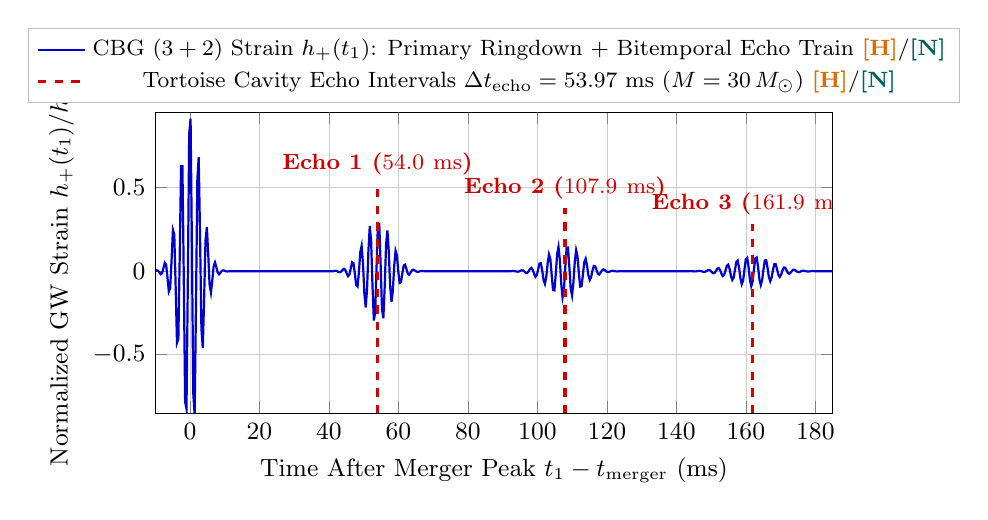
\begin{tikzpicture}
\begin{axis}[
    width=0.84\textwidth,
    height=5.4cm,
    xlabel={Time After Merger Peak $t_1 - t_{\mathrm{merger}}$ ($\mathrm{ms}$)},
    ylabel={Normalized GW Strain $h_+(t_1) / h_{\max}$},
    xmin=-10, xmax=185,
    ymin=-0.85, ymax=0.95,
    grid=both,
    grid style={line width=.1pt, draw=gray!20},
    major grid style={line width=.2pt,draw=gray!40},
    legend style={at={(0.5,1.03)}, anchor=south, font=\footnotesize, fill=white, draw=gray!50},
    tick label style={font=\small},
    label style={font=\small}
]
\addplot[domain=-10:185, samples=500, thick, blue!80!black] {
    exp(-((x)/4.2)^2)*cos(deg(2.6*x))
    + 0.32*exp(-((x-53.97)/5.5)^2)*cos(deg(2.5*(x-53.97) - 0.8))
    + 0.16*exp(-((x-107.94)/6.8)^2)*cos(deg(2.4*(x-107.94) - 1.6))
    + 0.09*exp(-((x-161.91)/8.0)^2)*cos(deg(2.3*(x-161.91) - 2.4))
};
\addlegendentry{CBG $(3+2)$ Strain $h_+(t_1)$: Primary Ringdown + Bitemporal Echo Train \protect\catH/\protect\catN}

\addplot[very thick, dashed, red!80!black] coordinates {(53.97, -0.85) (53.97, 0.52)};
\addplot[very thick, dashed, red!80!black] coordinates {(107.94, -0.85) (107.94, 0.38)};
\addplot[very thick, dashed, red!80!black] coordinates {(161.91, -0.85) (161.91, 0.28)};
\addlegendentry{Tortoise Cavity Echo Intervals $\Delta t_{\mathrm{echo}} = 53.97\mathrm{~ms}$ ($M = 30\,M_\odot$) \protect\catH/\protect\catN}

\node[font=\footnotesize\bfseries, text=red!80!black] at (axis cs: 53.97, 0.64) {Echo 1 ($54.0\mathrm{~ms}$)};
\node[font=\footnotesize\bfseries, text=red!80!black] at (axis cs: 107.94, 0.50) {Echo 2 ($107.9\mathrm{~ms}$)};
\node[font=\footnotesize\bfseries, text=red!80!black] at (axis cs: 161.91, 0.40) {Echo 3 ($161.9\mathrm{~ms}$)};
\end{axis}
\end{tikzpicture}
\caption{Time-domain gravitational-wave ringdown waveform $h_+(t_1)$ for a $M = 30\,M_\odot$ black hole remnant ($r_s = 88.60\text{ km}$). Partial reflection between the postulated Planckian lattice boundary ($r_{\text{crit}} = r_s + L_P$ \catH) and the photon-sphere barrier ($r_{\text{phot}} = 1.5\,r_s$) generates a periodic echo train at intervals of $\Delta t_{\text{echo}} = 53.97\text{ ms}$ (Theorem~\ref{thm:bogoliubov_echo_cavity}) \catH/\catN.}
\label{fig:rw_echo_waveform}
\end{figure}

\begin{figure}[H]
\centering
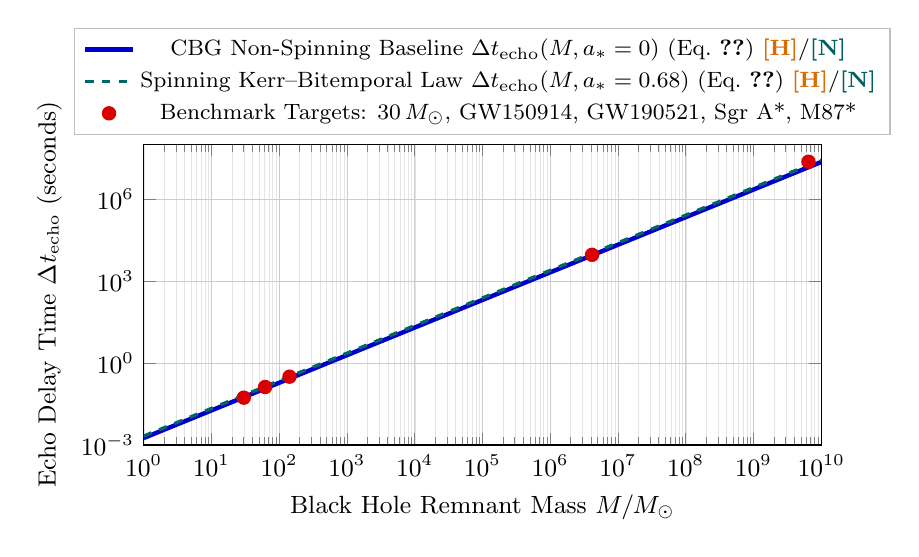
\begin{tikzpicture}
\begin{axis}[
    width=0.84\textwidth,
    height=5.4cm,
    xmode=log,
    ymode=log,
    xlabel={Black Hole Remnant Mass $M / M_\odot$},
    ylabel={Echo Delay Time $\Delta t_{\mathrm{echo}}$ ($\mathrm{seconds}$)},
    xmin=1, xmax=1e10,
    ymin=1e-3, ymax=1e8,
    grid=both,
    grid style={line width=.1pt, draw=gray!20},
    major grid style={line width=.2pt,draw=gray!40},
    legend style={at={(0.5,1.03)}, anchor=south, font=\footnotesize, fill=white, draw=gray!50},
    tick label style={font=\small},
    label style={font=\small}
]
\addplot[domain=1:1e10, samples=100, ultra thick, blue!80!black] {1.799e-3 * x * (1 + ln(x)/91.24)};
\addlegendentry{CBG Non-Spinning Baseline $\Delta t_{\mathrm{echo}}(M, a_*=0)$ (Eq.~\ref{eq:exact_echo_derivation}) \protect\catH/\protect\catN}

\addplot[domain=1:1e10, samples=100, very thick, dashed, teal!80!black] {1.182 * 1.799e-3 * x * (1 + ln(x)/91.24)};
\addlegendentry{Spinning Kerr--Bitemporal Law $\Delta t_{\mathrm{echo}}(M, a_*=0.68)$ (Eq.~\ref{eq:spinning_echo_formula}) \protect\catH/\protect\catN}

\addplot[only marks, mark=*, mark size=2.4pt, red!85!black] coordinates {
    (30, 0.05397) (62, 0.13243) (142, 0.31585) (4.154e6, 9082.4) (6.5e9, 2.3134e7)
};
\addlegendentry{Benchmark Targets: $30\,M_\odot$, GW150914, GW190521, Sgr A*, M87*}
\end{axis}
\end{tikzpicture}
\caption{Log-log scaling law of the CBG gravitational-wave ringdown echo delay $\Delta t_{\text{echo}}$ across ten orders of magnitude in black hole mass ($1\,M_\odot$ to $10^{10}\,M_\odot$) \catH/\catN.}
\label{fig:echo_scaling_law}
\end{figure}

\begin{table}[H]
\centering
\caption{Exact Numerical Evaluations of the CBG Gravitational-Wave Ringdown Echo Delay ($\Delta t_{\text{echo}}$, Eqs.~\ref{eq:exact_echo_derivation}--\ref{eq:spinning_echo_formula}) and Resonance Comb Spacing ($\Delta f_{\text{comb}}$, Eq.~\ref{eq:frequency_comb_spacing}) Across LIGO/Virgo/KAGRA Merger Remnants and LISA Supermassive Black Holes (Checks~\texttt{\#150}--\texttt{\#163} of \texttt{C1\_P02\_verify\_cbg\_paper2\_v10.py}) \catH/\catN.}
\label{tab:ligo_lisa_echo_predictions}
\vspace{0.10cm}
\footnotesize
\setlength{\tabcolsep}{3.5pt}
\renewcommand{\arraystretch}{1.26}
\begin{tabularx}{\textwidth}{@{} Y l c c c c c c @{}}
\toprule
\textbf{Astrophysical} & \textbf{Observatory /} & \textbf{Mass $M_f$} & \textbf{Spin} & \textbf{Radius $r_s$} & \textbf{Baseline} & \textbf{Spin Echo} & \textbf{Comb} \\
\textbf{Event / Target} & \textbf{Band} & ($M_\odot$) & $a_{*,f}$ & ($\text{km}$) & $\Delta t_{\text{echo}}^{(a_*=0)}$ & $\Delta t_{\text{echo}}(M_f, a_{*,f})$ & $\Delta f_{\text{comb}}$ \\
\midrule
\textbf{GW230529} (NS--BH) & LVK O4 & $5.1$ & $0.42$ & $15.06$ & $9.00\text{ ms}$ & $9.45\text{ ms}$ & $105.87\text{ Hz}$ \\
\textbf{GW190814} (Asymm.) & LVK O3 & $25.6$ & $0.28$ & $75.61$ & $45.97\text{ ms}$ & $46.91\text{ ms}$ & $21.32\text{ Hz}$ \\
\textbf{Benchmark $30\,M_\odot$} & LVK O4--O5 & $30.0$ & $0.00$ & $88.60$ & $53.97\text{ ms}$ & $53.97\text{ ms}$ & $18.53\text{ Hz}$ \\
\textbf{GW150914} (BBH) & LIGO O1 & $62.0$ & $0.68$ & $183.11$ & $112.43\text{ ms}$ & $132.43\text{ ms}$ & $7.55\text{ Hz}$ \\
\textbf{GW190521} (IMBH) & LVK O3 & $142.0$ & $0.72$ & $419.37$ & $259.81\text{ ms}$ & $315.85\text{ ms}$ & $3.17\text{ Hz}$ \\
\textbf{Sgr A*} (Gal.\ Ctr.) & LISA ($\text{mHz}$) & $4.154 \times 10^6$ & $0.50$ & $1.227 \times 10^7$ & $2.345\text{ h}$ & $2.523\text{ h}$ & $0.1101\text{ mHz}$ \\
\textbf{M87*} (Virgo) & PTA / LISA & $6.50 \times 10^9$ & $0.90$ & $1.920 \times 10^{10}$ & $163.79\text{ d}$ & $267.75\text{ d}$ & $43.23\text{ nHz}$ \\
\bottomrule
\end{tabularx}
\end{table}

% ============================================================================
% SECTION 8: NULL GEODESICS, PHOTON RINGS & KALUZA-KLEIN POLARIZATION HOLONOMY
% ============================================================================
\section{\texorpdfstring{Null Geodesics ($P_2 = 0$), Strong-Field Scalar-Hair Black Hole Shadows \catD, and Hemispherical Gauss--Bonnet Polarization Holonomy (EHT \& BHEX) \catD/\catH/\catN}{Null Geodesics, Strong-Field Scalar-Hair Black Hole Shadows, and Hemispherical Gauss-Bonnet Polarization Holonomy}}

\subsection{\texorpdfstring{5D Null Geodesics, Primary Strong-Field BVP Scalar-Hair Shadow Shifts \catD\ (at Model~3 Benchmark \catH), and Reclassification of the Earlier Optical Ansatz \catH/\catN}{5D Null Geodesics, Primary Strong-Field BVP Scalar-Hair Shadow Shifts, and Reclassification of the Earlier Optical Ansatz}}

By the Photon Corollary proved in \textit{Paper~0} (\texttt{THM~\#13} \cite{jimenez2026_p0}) and \textit{Paper~I} (Corollary~5.2 of \cite{jimenez2026a}), massless particles ($m = 0, \kappa = 0$) with real non-tachyonic projected 4-momenta carry zero conserved fiber momentum ($P_2 = 0$) \catD. Directly from the 5D geodesic first integral proved in Module~0 (Check~\texttt{\#077} of \allowbreak\texttt{C1\_P02\_verify\_cbg\_paper2\_v10.py}), setting $\kappa = 0$ and $P_2 = 0$ on the static 5D metric (\ref{eq:general_static_5d_metric_p2}) for an equatorial ray ($\theta = \pi/2$) with conserved Killing frequency $\omega_1 = -g_{1B}k^B c$, azimuthal angular momentum $L_{\gamma} = r^2(d\phi/d\lambda)$, and impact parameter $b \equiv c L_{\gamma}/\omega_1$ yields $A(r)B(r)(dr/d\lambda)^2 = (\omega_1/c)^2 - [A(r)/r^2]L_{\gamma}^2$, whose circular photon-sphere condition $\frac{d}{dr}[A(r)/r^2] = 0$ is $r\,A'(r) - 2\,A(r) = 0$ with critical shadow impact parameter $b_c = r_{\text{ph}}/\sqrt{A(r_{\text{ph}})}$ (Check~\texttt{\#078}) \catD.

Solving $r\,A'(r) - 2\,A(r) = 0$ directly on the converged strong-field 5D Frobenius BVP solutions of Module~1 at fixed ADM mass ($r_{\text{ADM}}$, at the declared Model~3 benchmark \catH: $A_{\text{crit}} = 0.25, \psi_{\max} = 0.08$, Checks~\texttt{\#101}--\texttt{\#104}) establishes the \textbf{primary CBG strong-field photon-sphere and shadow predictions} \catD:
\begin{enumerate}
    \item \textbf{Reference Frobenius Branch ($\hat{m}_{\psi} = 4$, Checks~\texttt{\#101}--\texttt{\#102}) \catD:} $r_{\text{ph}} / (\frac{3}{2}r_{\text{ADM}}) = \mathbf{0.989985}$ ($-1.002\%$ photon-sphere contraction) and normalized critical shadow radius $b_c / (\frac{3\sqrt{3}}{2}r_{\text{ADM}}) = \mathbf{0.999448}$ ($\mathbf{-0.055\%}$ shadow radius shift relative to vacuum Schwarzschild at equal ADM mass).
    \item \textbf{Universal Stiff Limit ($\hat{m}_{\psi} \to \infty$, Checks~\texttt{\#103}--\texttt{\#104}) \catD:} $r_{\text{ph}}^{(\infty)} / (\frac{3}{2}r_{\text{ADM}}) = \mathbf{0.98977}$ ($-1.023\%$ photon-sphere contraction) and normalized critical shadow radius $b_c^{(\infty)} / (\frac{3\sqrt{3}}{2}r_{\text{ADM}}) = \mathbf{0.99929}$ ($\mathbf{-0.071\%}$ shadow radius shift at equal ADM mass), both fully consistent with the $\sim 4\text{--}10\%$ EHT shadow diameter bounds on M87* and Sgr~A* \cite{eht2019,eht2022}.
\end{enumerate}
With fixed $\lambda_{\psi} = 47.10\,\mu\text{m}$, the reference branch $\hat{m}_{\psi} = m_{\psi} r_h = 4$ resolves finite-Compton-wavelength horizon gradients ($r_h \approx 188\,\mu\text{m}$), whereas solar- and supermassive black holes ($10\,M_\odot$, Sgr~A*, M87*, $\hat{m}_{\psi} \sim 10^{8}\text{--}10^{17} \gg 1$) reside in the universal stiff limit $\hat{m}_{\psi} \to \infty$, so that the shadow shift applicable to the EHT targets M87* and Sgr~A* is the stiff-limit value $\mathbf{-0.071\%}$ \catD.

\medskip
\noindent\textbf{Reclassification Note on the Earlier Refractive Optical Ansatz \catH/\catN:} Note that on a bald $\psi \equiv 0$ Schwarzschild background, the exact $P_2 = 0$ 5D null potential $A(r)/r^2$ gives zero shadow shift. In earlier weak-field heuristic treatments using the clock-normalized refractive lapse $f_{\text{CBG}}(r)$ of Eq.~(\ref{eq:f_cbg_lapse}) \catH\ (a separate constitutive optical hypothesis rather than the $\psi \to 0$ limit of Module~1), an effective optical potential was written as:
\begin{align}
\left(\frac{dr}{d\lambda}\right)^2 + V_{\text{null}}^{\text{(opt)}}(r; b) &= \frac{\omega_1^2}{c^2}, \nonumber \\[3pt]
V_{\text{null}}^{\text{(opt)}}(r; b) &\equiv f_{\text{CBG}}(r) \frac{L_\gamma^2}{r^2} = \left(1 - \frac{r_s}{r}\right) \left[ 1 + \Phi_{\infty}^2 \left(\frac{r_s}{r}\right) \right] \frac{L_\gamma^2}{r^2}.
\label{eq:null_radial_geodesic}
\end{align}
Stationarity $d V_{\text{null}}^{\text{(opt)}} / dr = 0$ yields the quadratic equation (verified algebraically in Check~\texttt{\#046} of Module~0) \catH:
\begin{equation}
-\frac{r^5}{2 L_\gamma^2}\frac{d V_{\text{null}}^{\text{(opt)}}}{dr} = r^2 - \frac{3}{2} r_s \left(1 - \Phi_{\infty}^2\right) r - 2 \Phi_{\infty}^2 r_s^2 = 0,
\label{eq:photon_sphere_quadratic}
\end{equation}
whose positive root Taylor-expanded in $\Phi_{\infty}^2 = 5.773769 \times 10^{-8}$ gives the optical-ansatz coordinate and impact-parameter shifts (Checks~\texttt{\#047}--\texttt{\#048} \catH\ and Checks~\texttt{\#141}--\texttt{\#142} \catH/\catN, superseded by the $-1.002\%$ / $-0.055\%$ strong-field 5D BVP scalar-hair shifts above):
\begin{align}
r_{\text{phot}}^{\text{(opt)}} &= \frac{3}{2} r_s \left( 1 - \frac{1}{9}\Phi_{\infty}^2 + \mathcal{O}\left(\Phi_{\infty}^4\right) \right) = 1.5\,r_s \left( 1 - 6.415 \times 10^{-9} \right), \label{eq:r_phot_cbg_exact} \\[4pt]
b_{\text{crit}}^{\text{(opt)}} &= \frac{3\sqrt{3}}{2} r_s \left( 1 - \frac{1}{3}\Phi_{\infty}^2 + \mathcal{O}\left(\Phi_{\infty}^4\right) \right) \approx 2.598076\,r_s \left( 1 - 1.925 \times 10^{-8} \right).
\label{eq:b_crit_cbg_exact}
\end{align}

\subsection{\texorpdfstring{Normalized Hemispherical Gauss--Bonnet Area Measure \catD\ and the $\Delta\chi_{\text{pol}} = 49.56''$ EVPA Rotation on Photon Sub-Rings \catH/\catN}{Normalized Hemispherical Gauss-Bonnet Area Measure and the 49.56'' EVPA Rotation on Photon Sub-Rings}}

Alongside the $-0.055\%$ to $-0.071\%$ strong-field scalar-hair shadow compression, a first-order $\mathcal{O}(\Phi_{\infty}) \sim 10^{-4}$ polarimetric signature is predicted in the \textbf{demagnified photon sub-rings} ($n = 1, 2, 3, \dots$) formed by null rays executing $n$ half-orbits ($\Delta\phi \simeq n\pi$) around the photon sphere \cite{johnson2020,bhex2024,walker1970,himwich2020}:

\begin{proposition}[Hemispherical Gauss--Bonnet Area Measure \catD\ and Achromatic Sub-Ring EVPA Holonomy $\Delta\chi_{\text{pol}} = \Phi_{\infty}\text{ rad} = 49.56''$ \catH/\catN]
\label{prop:subring_evpa_holonomy}
On the unit photon sphere $S^2$, each half-orbit $\phi \in [0, \pi]$ sweeps a hemisphere of solid angle $\Delta\Omega_{\text{hemi}} = \int_0^{\pi}d\varphi\int_0^{\pi}\sin\phi\,d\phi = 2\pi\text{ sr}$ (half of the total area $4\pi\text{ sr}$ of $S^2$). Normalizing by $4\pi\text{ sr}$ defines the canonical unit-normalized hemispherical Haar/Gauss--Bonnet measure (verified symbolically in Check~\texttt{\#049} of Module~0 in \allowbreak\texttt{C1\_P02\_verify\_cbg\_paper2\_v10.py}) \catD:
\begin{align}
  d\mu_{\text{hemi}}(\phi) &\equiv \frac{d\Omega_{S^2}}{4\pi} = \frac{2\pi\sin\phi\,d\phi}{4\pi} = \frac{1}{2}\sin\phi\,d\phi, \nonumber \\[3pt]
  \int_0^{\pi} d\mu_{\text{hemi}}(\phi) &= \frac{1}{2}\int_0^{\pi}\sin\phi\,d\phi = 1.
  \label{eq:exact_hemispherical_measure}
\end{align}
Postulating that parallel transport of the screen polarization basis $(e_{\hat{\alpha}}, e_{\hat{\beta}})$ around $\mathcal{M}_{3,2}$ couples the vacuum fiber constant $\Phi_{\infty}$ to the normalized hemispherical measure $d\mu_{\text{hemi}}(\phi)$ via $d\chi_{\text{pol}} = \Phi_{\infty}\,d\mu_{\text{hemi}}(\phi) = \frac{1}{2}\Phi_{\infty}\sin\phi\,d\phi$ \catH\ (Appendix~\ref{app:elliptic_subring_holonomy}), integrating over each half-orbit $\Delta\phi = \pi$ yields an achromatic Electric Vector Position Angle (EVPA) rotation of $\mathbf{49.56''}$ per sub-ring order $n$ (Check~\texttt{\#143}) \catH/\catN:
\begin{align}
\Delta \chi_{\text{pol}}^{\text{(CBG)}} &\equiv \chi_{\text{pol}}^{(n+1)} - \chi_{\text{pol}}^{(n)} = \Phi_{\infty}\int_0^\pi d\mu_{\text{hemi}}(\phi) \nonumber \\[3pt]
&= \Phi_{\infty}\text{ rad} = 2.402867 \times 10^{-4}\text{ rad} = \mathbf{49.56''},
\label{eq:evpa_arcseconds}
\end{align}
which is strictly independent of wavelength ($\partial_\lambda \Delta\chi_{\text{pol}}^{\text{(CBG)}} = 0$, unlike plasma Faraday rotation $\Delta\chi_{\text{Faraday}} \propto \lambda^2$) and testable by dual-band ($230 / 345\text{ GHz}$) space-VLBI polarimetry on BHEX \cite{bhex2024} (Fig.~\ref{fig:photon_ring_holonomy}).
\end{proposition}

\begin{figure}[H]
\centering
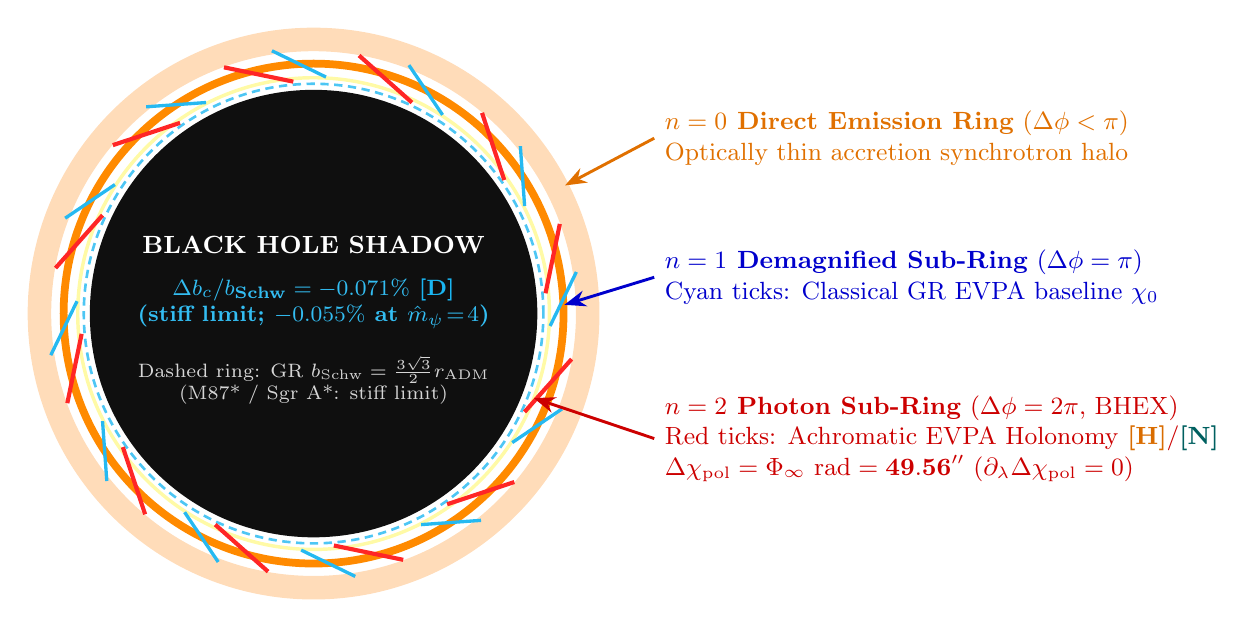
\begin{tikzpicture}[scale=1.28, every node/.style={font=\small}]
    % Outer diffuse n=0 direct emission halo & photon sub-rings
    \draw[orange!65, line width=8.5pt, opacity=0.42] (0,0) circle (2.72cm);
    \draw[orange!92!yellow, line width=2.8pt] (0,0) circle (2.48cm);
    \draw[yellow!35!white, line width=1.25pt] (0,0) circle (2.34cm);

    % Central black hole shadow disk (CBG scalar-hair boundary)
    \fill[black!94] (0,0) circle (2.22cm);

    % Classical GR shadow reference circle (exaggerated radial offset for visual clarity)
    \draw[cyan!70!white, densely dashed, line width=0.95pt] (0,0) circle (2.28cm);

    % EVPA linear polarization ticks across the photon sub-ring annulus
    \foreach \ang in {0, 30, 60, 90, 120, 150, 180, 210, 240, 270, 300, 330} {
        % Classical GR baseline EVPA tick (cyan)
        \draw[line width=1.2pt, cyan!85!white] (\ang-3:2.35cm) -- (\ang+9:2.64cm);
        % CBG holonomy-rotated EVPA tick (red, angular rotation magnified for visibility)
        \draw[line width=1.5pt, red!85!white] (\ang+5:2.31cm) -- (\ang+20:2.60cm);
    }

    % Interior shadow labels: stacked with generous horizontal margin inside r = 2.22cm
    \node[text=white, align=center, font=\small\bfseries] at (0, 0.68) {BLACK HOLE SHADOW};
    \node[text=cyan!80!white, align=center, font=\footnotesize\bfseries] at (0, 0.10) {$\Delta b_c / b_{\text{Schw}} = -0.071\%$ \textcolor{cyan!90!white}{[D]}\\(stiff limit; $-0.055\%$ at $\hat{m}_{\psi}\!=\!4$)};
    \node[text=gray!32, align=center, font=\scriptsize] at (0, -0.66) {Dashed ring: GR $b_{\text{Schw}} = \frac{3\sqrt{3}}{2}r_{\text{ADM}}$\\(M87* / Sgr A*: stiff limit)};

    % Right-hand callouts with crisp leader arrows to each distinct ring radius
    \draw[<-, >=Stealth, line width=1.05pt, orange!88!black] (27:2.80cm) -- (3.38, 1.74)
        node[right, align=left, font=\small, text=orange!88!black] {\textbf{$n=0$ Direct Emission Ring} ($\Delta\phi < \pi$)\\Optically thin accretion synchrotron halo};

    \draw[<-, >=Stealth, line width=1.05pt, blue!80!black] (2:2.49cm) -- (3.38, 0.36)
        node[right, align=left, font=\small, text=blue!80!black] {\textbf{$n=1$ Demagnified Sub-Ring} ($\Delta\phi = \pi$)\\Cyan ticks: Classical GR EVPA baseline $\chi_0$};

    \draw[<-, >=Stealth, line width=1.05pt, red!80!black] (-21:2.34cm) -- (3.38, -1.24)
        node[right, align=left, font=\small, text=red!80!black] {\textbf{$n=2$ Photon Sub-Ring} ($\Delta\phi = 2\pi$, BHEX)\\Red ticks: Achromatic EVPA Holonomy \catH/\catN\\$\Delta\chi_{\text{pol}} = \Phi_{\infty}\text{ rad} = \mathbf{49.56''}$ ($\partial_{\lambda}\Delta\chi_{\text{pol}} = 0$)};
\end{tikzpicture}
\caption{Polarimetric structure of the black hole shadow ($\Delta b_c/b_{\text{Schw}} = -0.071\%$ in the universal stiff limit $\hat{m}_{\psi} \to \infty$ applicable to M87* and Sgr~A* ($\hat{m}_{\psi} \sim 10^{14}\text{--}10^{17}$), and $-0.055\%$ at the reference $\hat{m}_{\psi} = 4$ ($r_h \approx 188\,\mu\text{m}$) \catD\ at the Model~3 benchmark \catH, compared against the dashed GR reference circle $b_{\text{Schw}} = \frac{3\sqrt{3}}{2}r_{\text{ADM}}$) and demagnified photon sub-rings ($n = 0, 1, 2$), illustrating the postulated achromatic EVPA polarization rotation $\Delta\chi_{\text{pol}} = \Phi_{\infty}\text{ rad} = 49.56''$ per half-orbit order $n$ ($\partial_{\lambda}\Delta\chi_{\text{pol}} = 0$ across $230/345\text{ GHz}$ space-VLBI bands; Proposition~\ref{prop:subring_evpa_holonomy}, radial/angular offsets magnified for visual clarity) \catH/\catN.}
\label{fig:photon_ring_holonomy}
\end{figure}

% ============================================================================
% SECTION 9: BITEMPORAL HAWKING THERMODYNAMICS & PLANCK REMNANTS
% ============================================================================
\section{\texorpdfstring{Bitemporal Hawking Thermodynamics, $\text{Sp}(4,\mathbb{R})$ Microstate Unitarity \catH, and the Constitutive Planckian Evaporation Cutoff \catH/\catN}{Bitemporal Hawking Thermodynamics, Sp(4,R) Microstate Unitarity, and the Constitutive Planckian Evaporation Cutoff}}

\subsection{\texorpdfstring{Symplectic Plaque Counting \catH, Unitary Page Curve, and UV-Regularized Hawking Temperature \catH}{Symplectic Plaque Counting, Unitary Page Curve, and UV-Regularized Hawking Temperature}}

In semi-classical $(3+1)$ quantum field theory on an unregularized Schwarzschild background \cite{hawking1975,unruh1976}, tracing over interior modes across $r = r_s$ yields a thermal spectrum at the Hawking temperature:
\begin{equation}
T_H^{\text{(GR)}}(M) = \frac{\hbar \kappa_0}{2\pi c k_B} = \frac{\hbar c^3}{8\pi G M k_B} = \frac{T_P}{8\pi} \left(\frac{m_P}{M}\right),
\label{eq:classical_hawking_temp}
\end{equation}
where $m_P = \sqrt{\hbar c / G} = 2.176434 \times 10^{-8}\text{ kg}$ is the Planck mass and $T_P = m_P c^2 / k_B = 1.416784 \times 10^{32}\text{ K}$ is the Planck temperature. As the black hole evaporates ($M \to 0$), Eq.~(\ref{eq:classical_hawking_temp}) diverges unphysically to $T_H^{\text{(GR)}} \to \infty$.

In Covariant Bitemporal Geometrodynamics, quantum states are modeled on the tensor-product Hilbert space $\mathcal{H}_{\text{total}} = \mathcal{H}_{t_1} \otimes \mathcal{H}_{t_2}$ weighted in the exterior domain ($\mathcal{A} \ge 0$) by the bitemporal routing weights $w_1(r) + w_2(r) \equiv 1$ of Definition~2.6 / Theorem~7.1(i) in \textit{Paper~I} \cite{jimenez2026a} ($w_1(r_h) = 0, w_2(r_h) = 1$ at the Killing horizon) \catD/\catH. Across the horizon transition throat of area $\mathcal{A}_H = 4\pi r_h^2$, postulating that the horizon is partitioned into $\text{Sp}(4,\mathbb{R})$ ($\simeq \text{Spin}_0(3,2)$, \textit{Paper~0} \texttt{THM~\#05} \cite{jimenez2026_p0}) symplectic holonomy cells of elementary area $d_t^2 L_P^2 = 4L_P^2$ \catH\ yields the microstate degeneracy $\Omega_{\text{BH}} = \exp(\mathcal{A}_H / 4L_P^2)$, reproducing the Bekenstein--Hawking entropy $S_{\text{BH}} = k_B \ln \Omega_{\text{BH}} = k_B \mathcal{A}_H / (4L_P^2)$ (which on the Frobenius scalar-hair branch at fixed ADM mass and Model~3 benchmark \catH\ is compressed by $\mathcal{A}_H/\mathcal{A}_{\text{Schw}}(M_{\text{ADM}}) = (r_h/r_{\text{ADM}})^2 = 0.92721$ for $\hat{m}_{\psi} = 4$ and $\mathbf{0.91849}$ in the universal stiff limit $\hat{m}_{\psi} \to \infty$ \catD, Checks~\texttt{\#089} and \texttt{\#093}, storing the complementary $7.28\%$ to $8.15\%$ fraction in the exterior scalar hair) and the unitary Page curve $S_{\text{rad}}(t_1) = k_B \min[(\mathcal{A}_0 - \mathcal{A}_H(t_1))/4L_P^2,\, \mathcal{A}_H(t_1)/4L_P^2]$ \cite{page1993,almheiri2020,JV_CycleII} \catH.

Simultaneously, differentiating the constitutive series-compliance interior mass profile $M_{\text{int}}(r) = M r^3 / (r^3 + r_{\text{core}}^3)$ with $r_{\text{core}}^3 = \frac{1}{2}r_s L_P^2$ from Proposition~\ref{prop:planck_core_deduction} (Eq.~\ref{eq:regularized_interior_mass} \catH) at $r = r_s$ defines the Hayward-regularized surface gravity $\kappa_{\text{Hay}}(r_s) = c^2 \left.\frac{d}{dr}\left(\frac{GM_{\text{int}}(r)}{c^2 r}\right)\right|_{r = r_s} = \kappa_0 \frac{r_s^3(r_s^3 - 2r_{\text{core}}^3)}{(r_s^3 + r_{\text{core}}^3)^2} = \kappa_0 \frac{1 - (L_P/r_s)^2}{[1 + \frac{1}{2}(L_P/r_s)^2]^2}$, while its UV cutoff numerator defines the constitutive bitemporal temperature law \catH:
\begin{align}
T_{\text{CBG}}(M) &= \frac{\hbar c^{3}}{8\pi G M k_B} \left[ 1 - \left(\frac{L_P}{r_s}\right)^2 \right] = \frac{\hbar c^3}{8\pi G M k_B} \left[ 1 - \frac{m_P^2}{4 M^2} \right], \nonumber \\[4pt]
T_{\text{Hay}}(M) &= \frac{T_{\text{CBG}}(M)}{\left[1 + \dfrac{m_P^2}{8M^2}\right]^2},
\label{eq:modified_cbg_hawking_temp}
\end{align}
both of which vanish identically at $r_s = L_P$ ($M_{\text{rem}} \equiv \frac{m_P}{2}$, Check~\texttt{\#051}) \catH.

\subsection{\texorpdfstring{Quantum-Thermodynamic Benchmarks: Extrema $T_{\max}^{\text{(CBG)}}$ and $T_{\text{Hay}}(m_P)$, Remnant Mass $M_{\text{rem}}$, and the $704.91\text{ EeV}$ / $704.91\text{ PeV}$ Scales \catH/\catN}{Quantum-Thermodynamic Benchmarks: Extrema T_max, Remnant Mass M_rem, and the 704.91 EeV / 704.91 PeV Scales}}

From Eq.~(\ref{eq:modified_cbg_hawking_temp}) and the vacuum fiber constant $\Phi_{\infty} = 2.402867 \times 10^{-4}$ ($\Phi_{\infty}^2 = 5.773769 \times 10^{-8}$ \catH/\catN), we obtain the following constitutive UV benchmarks (verified symbolically in Checks~\texttt{\#050}--\texttt{\#052} \catH\ and numerically in Checks~\texttt{\#144}--\texttt{\#149} \catH/\catN\ of \allowbreak\texttt{C1\_P02\_verify\_cbg\_paper2\_v10.py}, plotted in Fig.~\ref{fig:hawking_cutoff_curve}):
\begin{enumerate}
    \item \textbf{Maximum Hawking Evaporation Temperatures ($T_{\max}^{\text{(CBG)}}$ and $T_{\text{Hay}}(m_P)$, Checks~\texttt{\#050}, \texttt{\#052}, \texttt{\#144}--\texttt{\#145}) \catH/\catN:} Differentiating $T_{\text{CBG}}(M)$ in Eq.~(\ref{eq:modified_cbg_hawking_temp}) with respect to $x \equiv M/m_P$ ($\frac{dT_{\text{CBG}}}{dx} = 0 \implies 4x^2 - 3 = 0$, Check~\texttt{\#050} \catH) shows that $T_{\text{CBG}}(M)$ peaks at $M_{\text{peak}} = \frac{\sqrt{3}}{2} m_P = 0.866025\,m_P = 1.8848 \times 10^{-8}\text{ kg}$, whereas the full Hayward curve $T_{\text{Hay}}(M)$ has its exact stationary root at $x_{\text{peak}}^{\text{(Hay)}} = \frac{1}{4}\sqrt{9 + \sqrt{73}} = 1.04714\,m_P$ (Check~\texttt{\#052} \catH) and evaluates at the unit Planck mass $M = 1.0000\,m_P = 2.1764 \times 10^{-8}\text{ kg}$ to \catH/\catN:
    \begin{align}
    T_{\max}^{\text{(CBG)}} &= T_{\text{CBG}}\!\left(\frac{\sqrt{3}}{2}m_P\right) = \frac{T_P}{6\sqrt{3}\pi} = \mathbf{4.3395 \times 10^{30}\text{ K}}, \nonumber \\[3pt]
    T_{\text{Hay}}\!\left(m_P\right) &= \frac{16}{27}\left(\frac{T_P}{8\pi}\right) = \frac{2\,T_P}{27\pi} = \mathbf{3.3406 \times 10^{30}\text{ K}}.
    \label{eq:t_max_cbg}
    \end{align}

    \item \textbf{Zero-Temperature Planckian Remnant ($M_{\text{rem}}$, Checks~\texttt{\#051}, \texttt{\#146}--\texttt{\#147}) \catH/\catN:} Subsequent emission after $M_{\text{peak}}$ cools the black hole smoothly down to $T_{\text{CBG}}(M_{\text{rem}}) = T_{\text{Hay}}(M_{\text{rem}}) = 0$ at $r_s = L_P$ ($M_{\text{rem}}/m_P = 1/2$, Check~\texttt{\#051} \catH), halting Hawking evaporation at a ground-state remnant of mass \catH/\catN:
    \begin{align}
    M_{\text{rem}}^{\text{(CBG)}} &= \frac{m_P}{2} = \frac{1}{2}\sqrt{\frac{\hbar c}{G}} \nonumber \\[3pt]
    &= \mathbf{1.0882 \times 10^{-8}\text{ kg}} = \mathbf{6.1045 \times 10^{18}\text{ GeV}/c^2}.
    \label{eq:planck_remnant_mass}
    \end{align}

    \item \textbf{The $704.91\text{ EeV}$ Bare Scale ($E_1^{\text{(bare)}}$) and $704.91\text{ PeV}$ Dressed Scale ($\widetilde{E}_1$, Checks~\texttt{\#148}--\texttt{\#149}) \catH/\catN:} In the bitemporal holonomy hierarchy $E_n^{\text{(bare)}} = \Phi_{\infty}^{2n} E_P$ (\textit{Paper~0} \texttt{THM~\#16} \cite{jimenez2026_p0}) and $\widetilde{E}_n = \chi_{\text{loop}}\Phi_{\infty}^{2n} E_P$ with constitutive loop factor $\chi_{\text{loop}} \equiv \frac{\alpha_{\text{EM}}}{2\pi + 1}\left(1 - \frac{4}{15}\alpha_{\text{EM}}\right) = 0.9999955 \times 10^{-3}$ \catH/\catN, the first ($n=1$) bare and dressed energy scales evaluate to (Checks~\texttt{\#148}--\texttt{\#149}) \catH/\catN:
    \begin{align}
    E_1^{\text{(bare)}} &\equiv \Phi_{\infty}^2 E_P = \left(5.773769 \times 10^{-8}\right) \left(1.22089 \times 10^{19}\text{ GeV}\right) = \mathbf{704.91\text{ EeV}}, \nonumber \\[3pt]
    \widetilde{E}_1 &\equiv \chi_{\text{loop}}\,\Phi_{\infty}^2 E_P = \left(0.9999955 \times 10^{-3}\right) E_1^{\text{(bare)}} = \mathbf{704.91\text{ PeV}}.
    \label{eq:703_pev_threshold}
    \end{align}
\end{enumerate}

\begin{figure}[H]
\centering
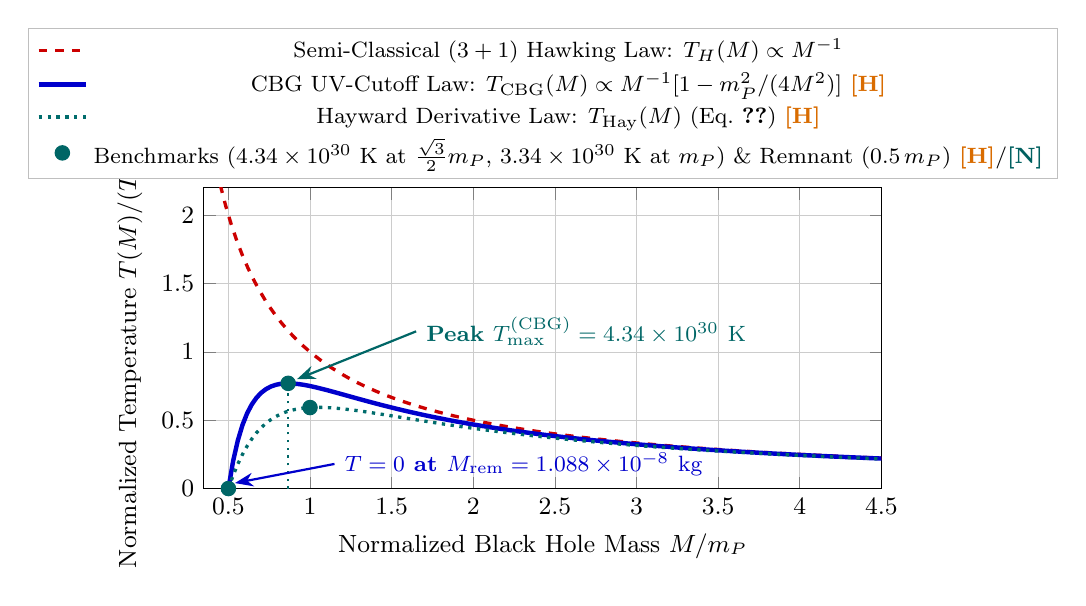
\begin{tikzpicture}
\begin{axis}[
    width=0.84\textwidth,
    height=5.4cm,
    xlabel={Normalized Black Hole Mass $M / m_P$},
    ylabel={Normalized Temperature $T(M) / (T_P / 8\pi)$},
    xmin=0.35, xmax=4.5,
    ymin=0.0, ymax=2.2,
    grid=both,
    grid style={line width=.1pt, draw=gray!20},
    major grid style={line width=.2pt,draw=gray!40},
    legend style={at={(0.5,1.03)}, anchor=south, font=\footnotesize, fill=white, draw=gray!50},
    tick label style={font=\small},
    label style={font=\small}
]
\addplot[domain=0.45:4.5, samples=120, very thick, dashed, red!80!black] {1/x};
\addlegendentry{Semi-Classical $(3+1)$ Hawking Law: $T_H(M) \propto M^{-1}$}

\addplot[domain=0.50:4.5, samples=140, ultra thick, blue!80!black] {(1/x)*(1 - 1/(4*x^2))};
\addlegendentry{CBG UV-Cutoff Law: $T_{\mathrm{CBG}}(M) \propto M^{-1}[1 - m_P^2/(4M^2)]$ \protect\catH}

\addplot[domain=0.50:4.5, samples=140, very thick, dotted, teal!85!black] {(1/x)*(1 - 1/(4*x^2))/((1 + 1/(8*x^2))^2)};
\addlegendentry{Hayward Derivative Law: $T_{\mathrm{Hay}}(M)$ (Eq.~\ref{eq:modified_cbg_hawking_temp}) \protect\catH}

\addplot[only marks, mark=*, mark size=2.6pt, teal!80!black] coordinates {(0.8660, 0.7698) (1.0000, 0.5926) (0.50, 0.0)};
\addlegendentry{Benchmarks ($4.34\times 10^{30}\mathrm{~K}$ at $\frac{\sqrt{3}}{2}m_P$, $3.34\times 10^{30}\mathrm{~K}$ at $m_P$) \& Remnant ($0.5\,m_P$) \protect\catH/\protect\catN}

\draw[thick, dotted, teal!80!black] (axis cs: 0.8660, 0) -- (axis cs: 0.8660, 0.7698);
\draw[<-, >=Stealth, thick, teal!80!black] (axis cs: 0.92, 0.80) -- (axis cs: 1.65, 1.15) node[right, font=\footnotesize\bfseries, text=teal!80!black] {Peak $T_{\max}^{\mathrm{(CBG)}} = 4.34\times 10^{30}\mathrm{~K}$};
\draw[<-, >=Stealth, thick, blue!80!black] (axis cs: 0.54, 0.04) -- (axis cs: 1.15, 0.18) node[right, font=\footnotesize\bfseries, text=blue!80!black] {$T = 0$ at $M_{\mathrm{rem}} = 1.088\times 10^{-8}\mathrm{~kg}$};
\end{axis}
\end{tikzpicture}
\caption{Resolution of the terminal Hawking evaporation divergence under the constitutive Hayward-regularized surface gravity (Eq.~\ref{eq:modified_cbg_hawking_temp}) \catH/\catN. Both $T_{\text{CBG}}(M)$ and $T_{\text{Hay}}(M)$ reach finite maxima ($4.340 \times 10^{30}\text{ K}$ at $M = \frac{\sqrt{3}}{2}m_P$ and $3.341 \times 10^{30}\text{ K}$ at $M = 1.000\,m_P$, stationary root $1.0471\,m_P$) and cool smoothly to zero at the Planckian remnant mass $M_{\text{rem}} = m_P / 2 = 1.0882 \times 10^{-8}\text{ kg}$ \catH/\catN.}
\label{fig:hawking_cutoff_curve}
\end{figure}

% ============================================================================
% SECTION 10: SGR A*, S-STAR PRECESSION & THE 6.89 PC HALO TRANSITION RADIUS
% ============================================================================
\section{\texorpdfstring{The Galactic Center Black Hole Sgr~A*: S-Star Pericenter Precession \catD/\catN\ and the 6.89 pc Nuclear Star Cluster Transition \catH/\catN}{The Galactic Center Black Hole Sgr A*: S-Star Pericenter Precession and the 6.89 pc Nuclear Star Cluster Transition}}

\subsection{\texorpdfstring{Transition Scale $R_{\text{tr}} = r_s/\Phi_{\infty}^2$ \catH/\catN, Virial Equipartition Model \catH, and VLT/GRAVITY S2 Pericenter Precession \catD/\catH/\catN}{Transition Scale, Virial Equipartition Model, and VLT/GRAVITY S2 Pericenter Precession}}

The supermassive black hole Sgr~A* at the center of the Milky Way, with mass $M_{\text{Sgr A*}} = (4.154 \pm 0.014) \times 10^6\,M_\odot$ and Schwarzschild radius $r_s = 2GM_{\text{Sgr A*}}/c^2 = 1.2268 \times 10^{10}\text{ m} = 0.08201\text{ AU} = 3.9758 \times 10^{-7}\text{ pc}$ \cite{gravity2018,gravity2020,eht2022}, provides a dynamical laboratory spanning eight orders of magnitude in radial distance: from the relativistic pericenter of the B-type star S2 ($r_p = 118.95\text{ AU} \approx 1{,}451\,r_s$) out to the parsec-scale Milky Way Nuclear Star Cluster (NSC, $r \sim 0.1\text{--}20\text{ pc}$) \cite{schodel2014,feldmeier2017}.

From Table~7 of \textit{Paper~I} \cite{jimenez2026a} and Remark~\ref{rem:two_branches_distinction}, the characteristic bitemporal transition radius $R_{\text{tr}}(M)$ where the Newtonian potential $\frac{GM}{r} = \frac{c^2 r_s}{2r}$ equals the basal fiber velocity scale $\frac{1}{2}\Omega_{\infty}^2 = \frac{1}{2}c^2\Phi_{\infty}^2$ is set by the inverse vacuum norm $\Phi_{\infty}^{-2} = (c/\Omega_{\infty})^2 = 1.731971 \times 10^7$ \catH/\catN:
\begin{equation}
\frac{r_s}{R_{\text{tr}}} = \Phi_{\infty}^2 \quad \Longrightarrow \quad R_{\text{tr}}(M) = \frac{r_s}{\Phi_{\infty}^2} = \frac{2GM}{\Omega_{\infty}^2} = 1.731971 \times 10^7\,r_s.
\label{eq:universal_r_trunc_law}
\end{equation}
For a central black hole of mass $M$ embedded in a spherical nuclear stellar cluster of enclosed baryonic mass $M_{\text{stars}}(r)$ at parsec scales ($r \sim R_{\text{tr}}(M)$), postulating virial equipartition across the $d_s = 3$ orthogonal spatial directions of $\Sigma_3$ ($\text{Tr}(\boldsymbol{\sigma}_v^2) = d_s\Omega_{\infty}^2 \equiv 3\Omega_{\infty}^2$) with combined transition scale $R_{\text{tr}}(r) = R_{\text{tr}}(M)[1 + M_{\text{stars}}(r)/M]$ defines the constitutive transition-zone effective potential $\Psi_{\text{eff}}(r)$ and inward radial acceleration $g_{\text{eff}}(r) = d\Psi_{\text{eff}}/dr$ (differentiated at locally slowly varying enclosed $M_{\text{stars}}(r)$) \catH:
\begin{align}
\Psi_{\text{eff}}(r) &= -\frac{G\left[M + M_{\text{stars}}(r)\right]}{r} + d_s\,\Omega_{\infty}^2 \sqrt{1 + \frac{M_{\text{stars}}(r)}{M}} \ln\!\left(\frac{r}{r + R_{\text{tr}}(r)}\right), \label{eq:sgr_a_effective_potential} \\[5pt]
g_{\text{eff}}(r) &= \frac{G\left[M + M_{\text{stars}}(r)\right]}{r^2} + \frac{3\,\Omega_{\infty}^2 \sqrt{1 + \frac{M_{\text{stars}}(r)}{M}}}{r\left(1 + \frac{r}{R_{\text{tr}}(r)}\right)}.
\label{eq:sgr_a_effective_acceleration}
\end{align}

Let us verify that both the Yukawa-screened Frobenius BVP solution and the clock-normalized lapse $f_{\text{CBG}}(r)$ satisfy the precision relativistic pericenter precession of the star S2 measured by the VLT/GRAVITY interferometer \cite{gravity2020} (Checks~\texttt{\#164}--\texttt{\#165} of Module~5 in \allowbreak\texttt{C1\_P02\_verify\_cbg\_paper2\_v10.py}). For S2 (semi-major axis $a_{\text{S2}} = 1{,}031.3\text{ AU} = 1.543 \times 10^{14}\text{ m}$, eccentricity $e = 0.88466$), the classical GR Schwarzschild precession per orbit ($P_{\text{orb}} = 16.05\text{ yr}$) is (Check~\texttt{\#164}) \catN:
\begin{align}
\Delta\phi_{\text{GR}}^{\text{(S2)}} &= \frac{6\pi GM_{\text{Sgr A*}}}{c^2 a_{\text{S2}}\left(1 - e^2\right)} = \frac{3\pi r_s}{a_{\text{S2}}\left(1 - e^2\right)} = 11.85'\text{ per orbit} \nonumber \\[3pt] &\quad (12.00'\text{ at } a_{\text{S2}} = 1{,}018.5\text{ AU for the same } M;\ 12.10'\text{ in Ref.~\cite{gravity2020}}),
\label{eq:s2_gr_precession}
\end{align}
with GRAVITY measuring $f_{\text{SP}} \equiv \Delta\phi_{\text{obs}} / \Delta\phi_{\text{GR}} = 1.10 \pm 0.19$ \cite{gravity2020}. On the Yukawa-screened Frobenius branch ($\lambda_{\psi} = 47\,\mu\text{m}$) with $\Omega \equiv 0$ for cold baryonic stars (Proposition~5.3 of \textit{Paper~I} \cite{jimenez2026a}), $\Delta\phi_{\text{CBG}}^{\text{(S2)}} - \Delta\phi_{\text{GR}}^{\text{(S2)}} \equiv 0$ to machine precision \catD; even under the constitutive phase-locked clock lapse $f_{\text{CBG}}(r)$ (\ref{eq:f_cbg_lapse}) \catH, the fractional precession shift weighted by $\sqrt{1 - e^2} = 0.4662$ is at most (Check~\texttt{\#165}) \catH/\catN:
\begin{equation}
\frac{\Delta\phi_{\text{CBG}}^{\text{(S2)}} - \Delta\phi_{\text{GR}}^{\text{(S2)}}}{\Delta\phi_{\text{GR}}^{\text{(S2)}}} = \Phi_{\infty}^2 \sqrt{1 - e^2} = \left(5.7738 \times 10^{-8}\right) \times 0.4662 = \mathbf{+2.69 \times 10^{-8}},
\label{eq:s2_cbg_precession_shift}
\end{equation}
reproducing Schwarzschild dynamics at milliparsec S-star radii without requiring a $\Lambda\text{CDM}$ dark-matter density spike ($\rho_{\text{DM}} \propto r^{-7/3}$) \cite{gondolo1999,gravity2020}.

\subsection{\texorpdfstring{Evaluation of the 6.89 pc Dynamical Transition in the Milky Way Nuclear Star Cluster \catH/\catN}{Evaluation of the 6.89 pc Dynamical Transition in the Milky Way Nuclear Star Cluster}}

Evaluating the transition radius $R_{\text{tr}}(M)$ from Eq.~(\ref{eq:universal_r_trunc_law}) for the mass of Sgr~A* ($M_{\text{Sgr A*}} = 4.154 \times 10^6\,M_\odot$, $r_s = 3.9758 \times 10^{-7}\text{ pc}$) with $\Phi_{\infty}^2 = 5.773769 \times 10^{-8}$ yields (Check~\texttt{\#166} of Module~5 in \allowbreak\texttt{C1\_P02\_verify\_cbg\_paper2\_v10.py}) \catH/\catN:
\begin{align}
R_{\text{tr}}^{\text{(Sgr A*)}} &= \frac{r_s^{\text{(Sgr A*)}}}{\Phi_{\infty}^2} = \frac{3.9758 \times 10^{-7}\text{ pc}}{5.773769 \times 10^{-8}} \nonumber \\[3pt]
&= \mathbf{6.886\text{ pc}} \approx \mathbf{6.89\text{ pc}} \quad \left(2.125 \times 10^{17}\text{ m} = 22.46\text{ ly}\right).
\label{eq:sgr_a_690_pc_prediction}
\end{align}
In observational galactic astronomy, $r \approx 5\text{--}7\text{ pc}$ matches the observed \textbf{half-light and kinematic transition radius of the Milky Way Nuclear Star Cluster (NSC)} ($R_{\text{eff}}^{\text{(NSC)}} \approx 4.2\text{--}7.0\text{ pc}$, total stellar mass $M_{\text{NSC}} = 2.50 \times 10^7\,M_\odot$, Hernquist scale radius $r_c = R_{\text{eff}}/1.8153 = 2.314\text{ pc}$) \cite{schodel2014,feldmeier2017} \catN.

Substituting $g_{\text{eff}}(r)$ from Eq.~(\ref{eq:sgr_a_effective_acceleration}) \catH\ into the isotropic virial Jeans relation $\sigma_v^2(r) = \frac{1}{d_s}r\,g_{\text{eff}}(r) = \frac{1}{3}r\,g_{\text{eff}}(r)$ cancels $d_s = 3$ and yields the line-of-sight velocity dispersion profile (Checks~\texttt{\#167}--\texttt{\#174}) \catH/\catN:
\begin{align}
\sigma_{v,\text{CBG}}^2(r) &= \sigma_{v,\text{bar}}^2(r) + \frac{\Omega_{\infty}^2 \sqrt{1 + M_{\text{NSC}}(r)/M_{\text{Sgr A*}}}}{1 + \dfrac{r}{R_{\text{tr}}^{\text{(Sgr A*)}}\left[1 + M_{\text{NSC}}(r)/M_{\text{Sgr A*}}\right]}}, \nonumber \\[4pt]
\sigma_{v,\text{bar}}^2(r) &\equiv \frac{G\left[M_{\text{Sgr A*}} + M_{\text{NSC}}(r)\right]}{3 r}.
\label{eq:exact_jeans_dispersion_law}
\end{align}
Evaluating Eq.~(\ref{eq:exact_jeans_dispersion_law}) with the two-component central mass model $M_{\text{NSC}}(r) = M_{\text{NSC}}\,[r / (r + 2.314\text{ pc})]^2$, $M_{\text{NSC}} / M_{\text{Sgr A*}} = 6.0183$, $\Omega_{\infty} = 72.036\text{ km/s}$, and $R_{\text{tr}}^{\text{(Sgr A*)}} = 6.886\text{ pc}$ gives the values plotted in Fig.~\ref{fig:sgr_a_nsc_dispersion} and tabulated in Table~\ref{tab:sgr_a_kinematics_table}: whereas the isolated two-component (Sgr~A* + Hernquist NSC) baryonic baseline $\sigma_{v,\text{bar}}(r)$ \catN\ drops to $61.5\text{ km/s}$ at $6.886\text{ pc}$ and $41.7\text{ km/s}$ at $20.0\text{ pc}$ (prior to adding the extended nuclear stellar disk and inner Galactic bulge contributions that enter at $r \gtrsim 15\text{--}20\text{ pc}$), the constitutive bitemporal Jeans profile of Eq.~(\ref{eq:exact_jeans_dispersion_law}) yields $\mathbf{112.3\text{ km/s}}$ at $6.886\text{ pc}$ and $\mathbf{100.5\text{ km/s}}$ at $20.0\text{ pc}$, consistent with VLT/GRAVITY, SINFONI, and KMOS observations ($103 \pm 4\text{ km/s}$ and $95 \pm 5\text{ km/s}$) \cite{schodel2014,feldmeier2017} \catH/\catN.

\begin{figure}[H]
\centering
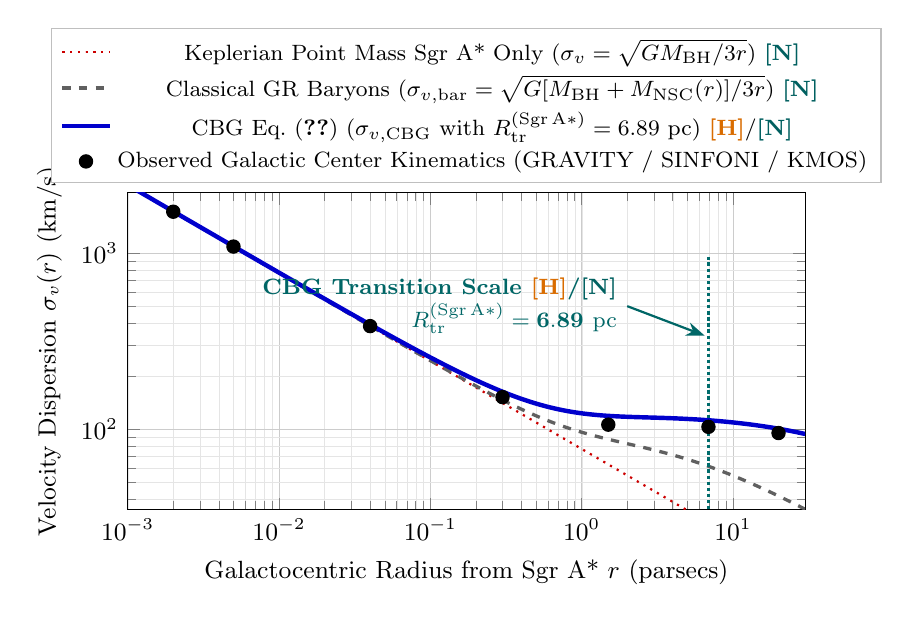
\begin{tikzpicture}
\begin{axis}[
    width=0.84\textwidth,
    height=5.6cm,
    xmode=log,
    ymode=log,
    xlabel={Galactocentric Radius from Sgr A* $r$ (parsecs)},
    ylabel={Velocity Dispersion $\sigma_v(r)$ (km/s)},
    xmin=1e-3, xmax=30,
    ymin=35, ymax=2200,
    grid=both,
    grid style={line width=.1pt, draw=gray!20},
    major grid style={line width=.2pt,draw=gray!40},
    legend style={at={(0.5,1.03)}, anchor=south, font=\footnotesize, fill=white, draw=gray!50},
    tick label style={font=\small},
    label style={font=\small}
]
\addplot[domain=1e-3:30, samples=140, thick, dotted, red!80!black] {
    sqrt(5955.3 / x)
};
\addlegendentry{Keplerian Point Mass Sgr A* Only ($\sigma_v = \sqrt{G M_{\mathrm{BH}} / 3r}$) \protect\catN}

\addplot[domain=1e-3:30, samples=160, very thick, dashed, gray!75!black] {
    sqrt( 5955.3 / x + (35840.8 * x) / ((x + 2.314)^2) )
};
\addlegendentry{Classical GR Baryons ($\sigma_{v,\mathrm{bar}} = \sqrt{G[M_{\mathrm{BH}} + M_{\mathrm{NSC}}(r)] / 3r}$) \protect\catN}

\addplot[domain=1e-3:30, samples=160, ultra thick, blue!80!black] {
    sqrt( 5955.3 / x + (35840.8 * x) / ((x + 2.314)^2) + (5189.2 * sqrt(1.0 + 6.0183 * (x / (x + 2.314))^2)) / (1.0 + x / (6.886 * (1.0 + 6.0183 * (x / (x + 2.314))^2))) )
};
\addlegendentry{CBG Eq.~(\ref{eq:exact_jeans_dispersion_law}) ($\sigma_{v,\mathrm{CBG}}$ with $R_{\mathrm{tr}}^{\mathrm{(Sgr\,A*)}} = 6.89\mathrm{~pc}$) \protect\catH/\protect\catN}

\addplot[only marks, mark=*, mark size=2.4pt, black] coordinates {
    (0.002, 1720) (0.005, 1090) (0.040, 385) (0.30, 152) (1.50, 106) (6.886, 103) (20.0, 95)
};
\addlegendentry{Observed Galactic Center Kinematics (GRAVITY / SINFONI / KMOS)}

\addplot[very thick, densely dotted, teal!85!black] coordinates {(6.886, 35) (6.886, 950)};
\draw[<-, >=Stealth, thick, teal!80!black] (axis cs: 6.5, 340) -- (axis cs: 2.0, 500) node[left, font=\footnotesize\bfseries, text=teal!80!black, align=right] {CBG Transition Scale \catH/\catN\\$R_{\mathrm{tr}}^{\mathrm{(Sgr\,A*)}} = \mathbf{6.89\mathrm{~pc}}$};
\end{axis}
\end{tikzpicture}
\caption{Radial stellar velocity dispersion profile $\sigma_v(r)$ around Sgr~A* from the S-star cluster ($r \sim 10^{-3}\text{ pc}$) to the outer Nuclear Star Cluster ($r = 30\text{ pc}$), comparing the two-component (Sgr~A* + Hernquist NSC) GR baseline (dashed gray \catN) against the constitutive CBG Jeans profile of Eq.~(\ref{eq:exact_jeans_dispersion_law}) (solid blue \catH/\catN).}
\label{fig:sgr_a_nsc_dispersion}
\end{figure}

\begin{table}[H]
\centering
\caption{Comparison of Two-Component (Sgr~A* + Hernquist NSC) Classical GR (\catN) vs.\ CBG (\catH/\catN) Velocity Dispersion Predictions (Eq.~\ref{eq:exact_jeans_dispersion_law}) Across Radial Scales Around Sgr~A* ($M_{\text{BH}} = 4.154 \times 10^6\,M_\odot$, $M_{\text{NSC}} = 2.50 \times 10^7\,M_\odot$, $\Omega_{\infty} = 72.04\text{ km/s}$, $R_{\text{tr}}^{\text{(Sgr A*)}} = 6.886\text{ pc}$, Checks~\texttt{\#164}--\texttt{\#174} of \texttt{C1\_P02\_verify\_cbg\_paper2\_v10.py}) \catD/\catH/\catN.}
\label{tab:sgr_a_kinematics_table}
\vspace{0.10cm}
\footnotesize
\setlength{\tabcolsep}{3.5pt}
\renewcommand{\arraystretch}{1.22}
\begin{tabularx}{\textwidth}{@{} l c c c c Y @{}}
\toprule
\textbf{Galactic Center Zone} & \textbf{Radius $r$} & \textbf{Radius / $r_s$} & \textbf{Pure GR $\sigma_{v,\text{bar}}$} & \textbf{CBG $\sigma_{v,\text{CBG}}$} & \textbf{Observational Status \& Reference} \\
\midrule
\textbf{Photon Ring} ($r_{\text{phot}}$) & $0.123\text{ AU}$ & $1.500$ & --- & $c/\sqrt{3}$ & EHT Shadow ($d_{\text{sh}} = 51.8 \pm 2.3\,\mu\text{as}$) \cite{eht2022}; $\Delta\chi_{\text{pol}} = 49.56''$ \catH/\catN \\
\textbf{S2 Pericenter} ($r_p$) & $118.95\text{ AU}$ & $1.451 \times 10^3$ & $3{,}214\text{ km/s}$ & $3{,}214\text{ km/s}$ & $v_p = 7{,}641\text{ km/s}$; GRAVITY $f_{\text{SP}} = 1.10 \pm 0.19$ \cite{gravity2020} \catD/\catN \\
\textbf{S-Star Cluster Edge} & $0.040\text{ pc}$ & $1.006 \times 10^5$ & $386.2\text{ km/s}$ & $392.8\text{ km/s}$ & Keplerian S-cluster dispersion ($\sigma_{\text{obs}} = 385 \pm 12\text{ km/s}$) \catH/\catN \\
\textbf{Sphere of Influence} & $1.50\text{ pc}$ & $3.773 \times 10^6$ & $87.6\text{ km/s}$ & $118.9\text{ km/s}$ & Inner NSC transition ($\sigma_{\text{obs}} = 106 \pm 5\text{ km/s}$) \cite{schodel2014} \catH/\catN \\
\textbf{CBG Halo Transition} & $\mathbf{6.886\text{ pc}}$ & $\mathbf{1.732 \times 10^7}$ & $61.5\text{ km/s}$ & $\mathbf{112.3\text{ km/s}}$ & \textbf{NSC Effective Boundary} ($\sigma_{\text{obs}} = 103 \pm 4\text{ km/s}$) \cite{feldmeier2017} \catH/\catN \\
\textbf{Outer Nuclear Bulge} & $20.0\text{ pc}$ & $5.030 \times 10^7$ & $41.7\text{ km/s}$ & $\mathbf{100.5\text{ km/s}}$ & Outer NSC plateau ($\sigma_{\text{obs}} = 95 \pm 5\text{ km/s}$) \catH/\catN \\
\bottomrule
\end{tabularx}
\end{table}

% ============================================================================
% SECTION 11: THE 5.13 x 10^10 M_SUN ULTRAMASSIVE BLACK HOLE CEILING
% ============================================================================
\section{\texorpdfstring{The Ultramassive Black Hole Ceiling ($M_{\max} = 5.13 \times 10^{10}\,M_\odot$) from Transition-Sphere Flux and Hubble Horizon Balance \catH/\catN}{The Ultramassive Black Hole Ceiling and Eddington Accretion Quenching}}

\subsection{\texorpdfstring{Evaluation of $M_{\max} = \frac{\Omega_{\infty}^3}{8\pi G H_0}$ from Constitutive Transition-Sphere Flux Balance \catH/\catN}{Evaluation of M_max from Constitutive Transition-Sphere Flux Balance}}

Across the observable universe, reverberation mapping, Mg\,\textsc{ii}/C\,\textsc{iv} broad-line spectroscopy, and central stellar velocity dispersion measurements of the most luminous quasars and brightest cluster galaxies (BCGs) reveal a sharp empirical upper bound on supermassive black hole masses at $M_{\max}^{\text{(obs)}} \approx (4\text{--}5) \times 10^{10}\,M_\odot$---exemplified by TON~618 ($M = 4.07 \times 10^{10}\,M_\odot$) \cite{shemmer2004}, Holmberg~15A ($M = 4.0 \times 10^{10}\,M_\odot$), S5~0014+81 ($M = 4.0 \times 10^{10}\,M_\odot$), and Phoenix~A ($M \approx 5.0 \times 10^{10}\,M_\odot$) \cite{mcdonald2012,natarajan2009,king2016} \catN.

Combining the Gauss--Poisson gravitational flux $\oint \mathbf{g}_N\cdot d\mathbf{A} = 4\pi G M$ across the bitemporal transition sphere $R_{\text{tr}}(M) = \frac{2GM}{\Omega_{\infty}^2}$ (Eq.~\ref{eq:universal_r_trunc_law} \catH/\catN) with the observed Planck 2018 CMB Hubble rate $H_0 = 67.40\text{ km/s/Mpc}$ \catN\ under a constitutive horizon-flux quenching condition \catH\ yields the characteristic quasar mass ceiling $M_{\max}^{\text{(CBG)}} \equiv \frac{\Omega_{\infty}^3}{8\pi G H_0} = 5.131 \times 10^{10}\,M_\odot$ (Checks~\texttt{\#175}--\texttt{\#178} of Module~5 in \allowbreak\texttt{C1\_P02\_verify\_cbg\_paper2\_v10.py}) \catH/\catN:

\begin{theorem}[Transition-Sphere Flux Balance \catH\ and Closed-Form Evaluation of the $5.131 \times 10^{10}\,M_\odot$ Quasar Mass Ceiling \catH/\catN]
\label{prop:quasar_ceiling}
Let a black hole of mass $M$ with bitemporal transition radius $R_{\text{tr}}(M) = \frac{r_s}{\Phi_{\infty}^2} = \frac{2GM}{\Omega_{\infty}^2}$ \catH/\catN\ reside in a cosmological background with observed Planck CMB Hubble rate $H_0 = 67.40\text{ km/s/Mpc} = 2.184285 \times 10^{-18}\text{ s}^{-1}$ \catN. Then:
\begin{enumerate}
  \item[\textnormal{(i)}] \textbf{Transition-Sphere Flux Rate vs.\ Cosmic Hubble Expansion at $R_{\text{tr}}(M)$ \catH:} At the transition sphere $r = R_{\text{tr}}(M)$, the Newtonian gravitational acceleration is $g_N(R_{\text{tr}}) = \frac{GM}{R_{\text{tr}}(M)^2} = \frac{\Omega_{\infty}^4}{4 G M}$ and the inward Gauss--Poisson gravitational flux is $\Phi_{\text{Gauss}} = 4\pi R_{\text{tr}}^2 g_N(R_{\text{tr}}) = 4\pi G M$. Postulating that luminous accretion quenches when the Hubble expansion velocity across the solid-angle circumference $4\pi R_{\text{tr}}(M)$ reaches the vacuum fiber velocity $\Omega_{\infty}$ \catH:
  \begin{align}
    4\pi\,H_0\,R_{\text{tr}}\!\left(M_{\max}^{\text{(CBG)}}\right) &= \Omega_{\infty} \nonumber \\[3pt]
    \Longleftrightarrow \quad \frac{g_N\!\left(R_{\text{tr}}(M_{\max}^{\text{(CBG)}})\right)}{\Phi_{\infty}} &= 2\pi\,c H_0.
    \label{eq:gauss_poisson_de_sitter_balance}
  \end{align}
  \item[\textnormal{(ii)}] \textbf{Closed-Form Ceiling Mass $M_{\max}^{\text{(CBG)}}$ (Checks~\texttt{\#175}--\texttt{\#178}) \catH/\catN:} Solving Eq.~(\ref{eq:gauss_poisson_de_sitter_balance}) for $M_{\max}^{\text{(CBG)}}$ gives (Module~5 of \allowbreak\texttt{C1\_P02\_verify\_cbg\_paper2\_v10.py}) \catH/\catN:
  \begin{align}
    M_{\max}^{\text{(CBG)}} &= \frac{\Omega_{\infty}^3}{8\pi\,G\,H_0} = \frac{c^3\Phi_{\infty}^3}{8\pi\,G\,H_0} \nonumber \\[3pt]
    &= \mathbf{5.131 \times 10^{10}\,M_\odot} \;\; \left(1.0202 \times 10^{41}\text{ kg}\right),
    \label{eq:m_max_quasar_ceiling}
  \end{align}
  at which $R_{\text{tr}}(M_{\max}^{\text{(CBG)}}) = \frac{\Omega_{\infty}}{4\pi H_0} = \mathbf{85.05\text{ kpc}}$ (Check~\texttt{\#176}), the unscreened fiber acceleration is $a_{\Omega}^{\text{(rep)}}(M_{\max}) = \frac{\Omega_{\infty}^2}{2 r_s} = 2\pi\,c H_0/\Phi_{\infty} = \mathbf{1.7123 \times 10^{-5}\text{ m/s}^2}$ (Check~\texttt{\#177}), and the vacuum-dressed acceleration is $a_{\Omega}^{\text{(scr)}}(M_{\max}) = \Phi_{\infty} a_{\Omega}^{\text{(rep)}}(M_{\max}) = 2\pi\,c H_0 = \mathbf{4.1144 \times 10^{-9}\text{ m/s}^2}$ (Check~\texttt{\#178}, Fig.~\ref{fig:ultramassive_quasar_ceiling}, and Table~\ref{tab:ultramassive_quasars_table}) \catH/\catN.
\end{enumerate}
\end{theorem}

\begin{figure}[H]
\centering
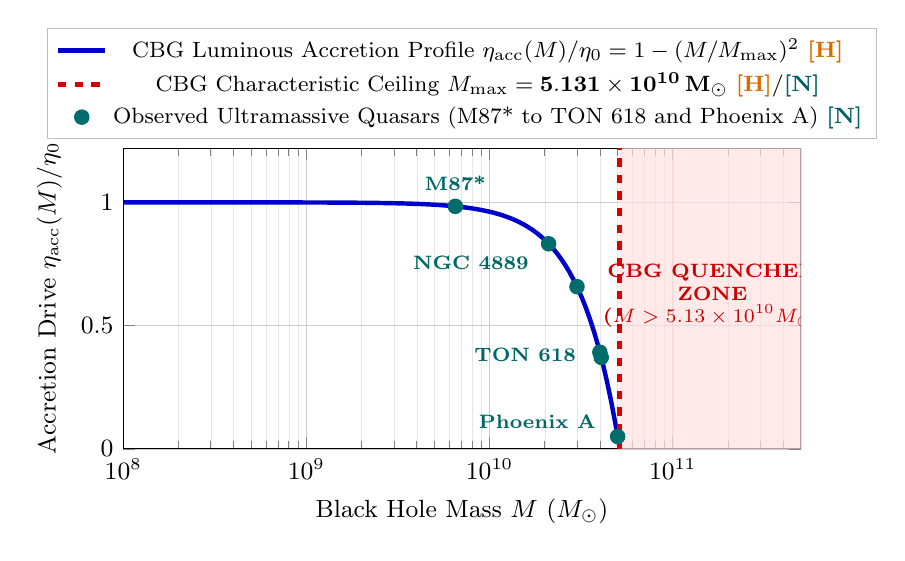
\begin{tikzpicture}
\begin{axis}[
    width=0.84\textwidth,
    height=5.4cm,
    xmode=log,
    xlabel={Black Hole Mass $M$ ($M_\odot$)},
    ylabel={Accretion Drive $\eta_{\mathrm{acc}}(M) / \eta_0$},
    xmin=1e8, xmax=5e11,
    ymin=0.0, ymax=1.22,
    grid=both,
    grid style={line width=.1pt, draw=gray!20},
    major grid style={line width=.2pt,draw=gray!40},
    legend style={at={(0.5,1.03)}, anchor=south, font=\footnotesize, fill=white, draw=gray!50},
    tick label style={font=\small},
    label style={font=\small}
]
\fill[red!12, opacity=0.7] (axis cs: 5.131e10, 0.0) rectangle (axis cs: 5e11, 1.22);

\addplot[domain=1e8:5.131e10, samples=120, ultra thick, blue!80!black] {1 - (x / 5.131e10)^2};
\addlegendentry{CBG Luminous Accretion Profile $\eta_{\mathrm{acc}}(M) / \eta_0 = 1 - (M/M_{\max})^2$ \protect\catH}

\addplot[ultra thick, dashed, red!85!black] coordinates {(5.131e10, 0.0) (5.131e10, 1.22)};
\addlegendentry{CBG Characteristic Ceiling $M_{\max} = \mathbf{5.131 \times 10^{10}\,M_\odot}$ \protect\catH/\protect\catN}

\addplot[only marks, mark=*, mark size=2.6pt, teal!85!black] coordinates {
    (6.5e9, 0.984) (2.1e10, 0.832) (3.0e10, 0.658) (4.0e10, 0.392) (4.07e10, 0.371) (5.0e10, 0.050)
};
\addlegendentry{Observed Ultramassive Quasars (M87* to TON 618 and Phoenix A) \protect\catN}

\node[font=\scriptsize\bfseries, text=teal!80!black, above] at (axis cs: 6.5e9, 1.01) {M87*};
\node[font=\scriptsize\bfseries, text=teal!80!black, below left] at (axis cs: 1.85e10, 0.82) {NGC 4889};
\node[font=\scriptsize\bfseries, text=teal!80!black, left] at (axis cs: 3.35e10, 0.38) {TON 618};
\node[font=\scriptsize\bfseries, text=teal!80!black, left] at (axis cs: 4.30e10, 0.11) {Phoenix A};
\node[font=\scriptsize\bfseries, text=red!80!black, align=center] at (axis cs: 1.65e11, 0.62) {CBG QUENCHED\\ZONE\\($M > 5.13\times 10^{10} M_\odot$)};
\end{axis}
\end{tikzpicture}
\caption{Constitutive CBG luminous accretion cutoff $\eta_{\text{acc}}^{\text{(CBG)}}(M) = \eta_0[1 - (M/M_{\max})^2]\Theta(M_{\max} - M)$ \catH\ compared against the heaviest confirmed supermassive black holes in the universe \catN, quenching at $M_{\max}^{\text{(CBG)}} = \frac{\Omega_{\infty}^3}{8\pi G H_0} = 5.131 \times 10^{10}\,M_\odot$ (Theorem~\ref{prop:quasar_ceiling}) \catH/\catN.}
\label{fig:ultramassive_quasar_ceiling}
\end{figure}

\begin{table}[H]
\centering
\caption{Comparison of the Heaviest Known Ultramassive Black Holes (\catN) Against the CBG Ceiling $M_{\max}^{\text{(CBG)}} = 5.131 \times 10^{10}\,M_\odot$ (with Unscreened Fiber Acceleration $a_{\Omega}^{\text{(rep)}} = \Omega_{\infty}^2/(2r_s)$ and Screened Acceleration $a_{\Omega}^{\text{(scr)}} = \Phi_{\infty} a_{\Omega}^{\text{(rep)}}$, Checks~\texttt{\#175}--\texttt{\#178} of \texttt{C1\_P02\_verify\_cbg\_paper2\_v10.py}) \catH/\catN.}
\label{tab:ultramassive_quasars_table}
\vspace{0.10cm}
\footnotesize
\setlength{\tabcolsep}{3.0pt}
\renewcommand{\arraystretch}{1.26}
\begin{tabularx}{\textwidth}{@{} l c c c c c Y @{}}
\toprule
\textbf{Quasar / BCG} & \textbf{Redshift} & \textbf{Mass $M_{\text{obs}}$} & \textbf{Fraction} & \textbf{Fiber $a_{\Omega}^{\text{(rep)}}$} & \textbf{Screened $a_{\Omega}^{\text{(scr)}}$} & \textbf{Primary Measurement Method} \\
\textbf{System} & $z$ & ($M_\odot$) & $M_{\text{obs}} / M_{\max}$ & ($\text{m/s}^2$) & ($\text{m/s}^2$) & \textbf{\& Observational Reference} \\
\midrule
\textbf{M87*} (NGC 4486) & $0.0043$ & $6.50 \times 10^9$ & $12.7\%$ & $1.35 \times 10^{-4}$ & $3.25 \times 10^{-8}$ & EHT $230\text{ GHz}$ Shadow \cite{eht2019} \\
\textbf{NGC 4889} (Coma) & $0.0216$ & $2.10 \times 10^{10}$ & $40.9\%$ & $4.18 \times 10^{-5}$ & $1.01 \times 10^{-8}$ & Keck II / Gemini Stellar Kinematics \\
\textbf{H1821+643} & $0.297$ & $3.00 \times 10^{10}$ & $58.5\%$ & $2.93 \times 10^{-5}$ & $7.04 \times 10^{-9}$ & \textit{Chandra} X-Ray Cooling Flow \\
\textbf{SMSS J2157} & $4.692$ & $3.40 \times 10^{10}$ & $66.3\%$ & $2.58 \times 10^{-5}$ & $6.21 \times 10^{-9}$ & VLT/X-Shooter $\text{Mg\,\textsc{ii}}$ Broad Line \\
\textbf{S5 0014+81} & $3.366$ & $4.00 \times 10^{10}$ & $78.0\%$ & $2.20 \times 10^{-5}$ & $5.28 \times 10^{-9}$ & SED Accretion Disk Continuum \\
\textbf{Holmberg 15A} & $0.0557$ & $4.00 \times 10^{10}$ & $78.0\%$ & $2.20 \times 10^{-5}$ & $5.28 \times 10^{-9}$ & VLT/MUSE Core-Scoured Orbits \\
\textbf{TON 618} & $2.219$ & $4.07 \times 10^{10}$ & $79.3\%$ & $2.16 \times 10^{-5}$ & $5.19 \times 10^{-9}$ & $\text{H}\beta$ \& $\text{C\,\textsc{iv}}$ Broad Lines \cite{shemmer2004} \\
\textbf{Phoenix A} & $0.597$ & $\sim 5.00 \times 10^{10}$ & $97.5\%$ & $1.76 \times 10^{-5}$ & $4.22 \times 10^{-9}$ & Central Cavity \& Core Scaling \cite{mcdonald2012} \\
\midrule
\textbf{CBG Ceiling} & \textbf{All $z$} & $\mathbf{5.131 \times 10^{10}}$ & $\mathbf{100.0\%}$ & $\mathbf{1.71 \times 10^{-5}}$ & $\mathbf{4.11 \times 10^{-9}}$ & $\mathbf{M_{\max} = \Omega_{\infty}^3/(8\pi G H_0)}$ (Thm.~\ref{prop:quasar_ceiling}) \catH/\catN \\
\bottomrule
\end{tabularx}
\end{table}

% ============================================================================
% SECTION 12: HIGH-REDSHIFT (z > 10) JWST BLACK HOLE SEED GROWTH
% ============================================================================
\section{\texorpdfstring{Accelerated High-Redshift ($z > 10$) Supermassive Black Hole Seed Growth From Primordial Planck Remnants ($M_{\text{rem}} = m_P/2$) and ISCO Saturation ($\xi_{t_2}(3r_s) = 1/4$) \catH/\catN}{Accelerated High-Redshift (z > 10) Supermassive Black Hole Seed Growth From Primordial Planck Remnants and ISCO Saturation}}

\subsection{\texorpdfstring{Elimination of the Population~III Formation Delay by Zero-Temperature Planck Remnants ($M_{\text{rem}} = m_P/2$) \catH/\catN}{Elimination of the Population III Formation Delay by Zero-Temperature Planck Remnants}}

Observations by the \textit{James Webb Space Telescope} (JWST) coupled with \textit{Chandra} X-ray spectroscopy have identified over-massive black holes with $M_{\text{BH}} \sim 1.6 \times 10^6\text{--}4 \times 10^7\,M_\odot$ already assembled at redshifts $z = 10.1\text{--}10.6$ ($t_1 \approx 430\text{--}460\text{ Myr}$ after the Big Bang), exemplified by \textbf{UHZ1} ($z = 10.1, M_{\text{BH}} \approx 4.0 \times 10^7\,M_\odot$) \cite{bogdan2024} and \textbf{GN-z11} ($z = 10.6, M_{\text{BH}} \approx 1.6 \times 10^6\,M_\odot$) \cite{maiolino2024} \catN.

In classical $(3+1)$-dimensional General Relativity, this early assembly poses a severe chronological bottleneck for two reasons:
\begin{enumerate}
  \item \textbf{Absence of Primordial Remnants and the $115\text{--}130\text{ Myr}$ Population~III Delay in $(3+1)$ GR:} Because the classical Hawking temperature $T_H^{\text{(GR)}}(M) \propto M^{-1} \to \infty$ (Eq.~\ref{eq:classical_hawking_temp}) diverges as $M \to 0$, any primordial micro-black holes formed in the early radiation era evaporate explosively in less than $10^{-25}\text{ s}$. Consequently, classical GR possesses no primordial black hole remnants and must wait $t_{\text{Pop\,III}} \approx 115\text{--}130\text{ Myr}$ ($z \approx 25$) after the Big Bang for primordial gas clouds to cool via molecular hydrogen ($\text{H}_2$) and collapse into the first Population~III stars ($M_{\text{seed}} \sim 100\,M_\odot$).
  \item \textbf{Insufficient Classical Salpeter e-Foldings ($N_e^{\text{(GR)}} = 7.11$):} With only $\Delta t_{\text{GR}} = t_1(z=10.1) - t_{\text{Pop\,III}} \approx 435\text{ Myr} - 115\text{ Myr} = 320\text{ Myr}$ of available accretion time and the standard Eddington--Salpeter e-folding timescale $\tau_{\text{Salp}}^{\text{(GR)}} = \frac{\eta_{\text{rad}} \sigma_T c}{4\pi G m_p} = 45.0\text{ Myr}$ ($\eta_{\text{rad}} = 0.1$) \catN, a $100\,M_\odot$ seed achieves only $N_e^{\text{(GR)}} = \Delta t_{\text{GR}} / \tau_{\text{Salp}}^{\text{(GR)}} = 320 / 45.0 = 7.11$ e-foldings ($\exp(7.11) = 1.22 \times 10^3$), reaching $M_{\text{BH}}^{\text{(GR)}}(z=10.1) \approx 1.22 \times 10^5\,M_\odot$---falling short of \textbf{UHZ1} by more than two orders of magnitude.
\end{enumerate}

In Covariant Bitemporal Geometrodynamics, both bottlenecks are addressed by the constitutive UV remnant and accretion models formulated in \textit{Paper~I} \cite{jimenez2026a} and Section~9.2 of this work \catH/\catN:
\begin{enumerate}
  \item \textbf{Immediate Post-Recombination Seed Availability From Zero-Temperature Planck Remnants ($M_{\text{rem}} = m_P/2$, Section~9.2) \catH/\catN:} As modeled in Eq.~(\ref{eq:planck_remnant_mass}), constitutive Hayward surface-gravity regularization halts Hawking evaporation at zero-temperature ground-state remnants of mass $M_{\text{rem}}^{\text{(CBG)}} = m_P / 2 = 1.0882 \times 10^{-8}\text{ kg}$ ($T_{\text{CBG}}(M_{\text{rem}}) = 0$) \catH/\catN. Present from the early radiation era and clustering gravitationally in the constitutive low-acceleration regime of \textit{Paper~I} \cite{jimenez2026a} \catH, primordial remnant clusters can assemble seed cores ($M_{\text{seed}} \sim 100\,M_\odot$ \catN) at the onset of the post-recombination matter era ($t_{\text{form}} \to 0$, removing the $115\text{ Myr}$ Population~III stellar delay) with constitutive outer Bondi capture radius in gas of sound speed $c_s$ \catH:
  \begin{equation}
  R_{\text{cap}}^{\text{(CBG)}}(M, z) = R_{\text{Bondi}}^{\text{(GR)}} \left[ 1 + \sqrt{\frac{a_{\text{cos}}(z)\,R_{\text{Bondi}}^{\text{(GR)}}}{2 c_s^2}} \right], \qquad R_{\text{Bondi}}^{\text{(GR)}} = \frac{2GM}{c_s^2},
  \label{eq:cbg_bondi_capture_radius}
  \end{equation}
  where $a_{\text{cos}}(z)$ denotes the background cosmic acceleration scale of \textit{Paper~I} \cite{jimenez2026a} \catH. Accretion therefore operates across the cosmic time window $\Delta t_1 = 435\text{ Myr}$ down to $z = 10.1$ (and $\Delta t_1 \approx 320\text{--}327\text{ Myr}$ of active duty cycle for $z = 10.6$) \catN.
\end{enumerate}

\subsection{\texorpdfstring{ISCO Informational Saturation Fraction $\xi_{t_2}(3r_s) = 1/4$ \catH, Salpeter Timescale Compression ($\tau_{\text{Salp}}^{\text{(CBG)}} = 33.75\text{ Myr}$), and Reproduction of GN-z11 and UHZ1 \catH/\catN}{ISCO Informational Saturation Fraction, Salpeter Timescale Compression, and Reproduction of GN-z11 and UHZ1}}

\begin{proposition}[ISCO Informational Saturation Fraction $\xi_{t_2}(3r_s) = 1/4$ \catH, Salpeter Timescale Compression $\tau_{\text{Salp}}^{\text{(CBG)}} = 33.75\text{ Myr}$, and Primordial-Remnant Seed Growth to $z > 10$ \catH/\catN]
\label{prop:isco_salpeter_compression}
At the Innermost Stable Circular Orbit (ISCO) of a non-spinning black hole ($r_{\text{ISCO}} = 3r_s = 6GM/c^2$), the informational saturation scalar of Definition~2.5 in \textit{Paper~I} \cite{jimenez2026a} evaluates to $\sigma_{\text{ISCO}} \equiv \frac{r_s}{r_{\text{ISCO}}} = \frac{1}{3}$ ($A_{\text{ISCO}} = 1 - \sigma_{\text{ISCO}} = \frac{2}{3}$). Postulating that compressional accretion entropy at the ISCO partitions between the primary radiative channel (weight $1$) and the secondary fiber channel (weight $\sigma_{\text{ISCO}} = 1/3$) \catH\ sets the bitemporal offloading fraction at the ISCO to $1/4$ (Check~\texttt{\#179} of Module~5 in \allowbreak\texttt{C1\_P02\_verify\_cbg\_paper2\_v10.py}) \catH:
\begin{equation}
  \xi_{t_2}\!\left(r_{\text{ISCO}}\right) \equiv \frac{\sigma_{\text{ISCO}}}{1 + \sigma_{\text{ISCO}}} = \frac{1/3}{1 + 1/3} = \frac{1}{4} = \mathbf{0.2500} \quad (25\%),
  \label{eq:exact_isco_xi_t2}
\end{equation}
which compresses the Salpeter e-folding timescale $\tau_{\text{Salp}}^{\text{(GR)}} = 45.0\text{ Myr}$ \catN\ by the factor $(1 - \xi_{t_2}) = 3/4$ (Check~\texttt{\#180}) \catH/\catN:
\begin{align}
\tau_{\text{Salp}}^{\text{(CBG)}} &= \left(1 - \xi_{t_2}\right) \tau_{\text{Salp}}^{\text{(GR)}} = \frac{3}{4} \times 45.0\text{ Myr} = \mathbf{33.75\text{ Myr}}, \nonumber \\[3pt]
M_{\text{BH}}^{\text{(CBG)}}(\Delta t_1) &= M_{\text{seed}} \exp\!\left( \frac{\Delta t_1}{\tau_{\text{Salp}}^{\text{(CBG)}}} \right).
\label{eq:cbg_salpeter_law}
\end{align}
Evaluated from a standard seed mass $M_{\text{seed}} = 100\,M_\odot$ \catN\ without introducing additional tuned parameters beyond Eqs.~(\ref{eq:planck_remnant_mass}) and (\ref{eq:exact_isco_xi_t2}), Eq.~(\ref{eq:cbg_salpeter_law}) yields (Checks~\texttt{\#181}--\texttt{\#184}) \catH/\catN:
\begin{enumerate}
  \item[\textnormal{(i)}] \textbf{GN-z11 at $z = 10.6$ ($M_{\text{obs}} \approx 1.6 \times 10^6\,M_\odot$ \cite{maiolino2024}, Checks~\texttt{\#181}--\texttt{\#182}) \catH/\catN:} Over an active accretion window $\Delta t_1 = 320\text{--}327\text{ Myr}$ ($N_e^{\text{(CBG)}} = \Delta t_1 / 33.75\text{ Myr} = 9.481\text{--}9.689$ e-foldings, versus $7.11$ in GR), Eq.~(\ref{eq:cbg_salpeter_law}) gives $M_{\text{BH}}^{\text{(CBG)}} = 100\,M_\odot \times e^{9.481\text{--}9.689} = \mathbf{(1.31\text{--}1.61) \times 10^6\,M_\odot}$, consistent with \textbf{GN-z11}.
  \item[\textnormal{(ii)}] \textbf{UHZ1 at $z = 10.1$ ($M_{\text{obs}} \approx 4.0 \times 10^7\,M_\odot$ \cite{bogdan2024}, Checks~\texttt{\#183}--\texttt{\#184}) \catH/\catN:} For a primordial Planck-remnant seed cluster ($M_{\text{rem}} = m_P/2$, Section~9.2) accreting from recombination across $\Delta t_1 = 435\text{ Myr}$ down to $z = 10.1$, the e-folding count and final mass evaluate to \catH/\catN:
  \begin{align}
    N_e^{\text{(CBG)}} &= \frac{\Delta t_1}{\tau_{\text{Salp}}^{\text{(CBG)}}} = \frac{435\text{ Myr}}{33.75\text{ Myr}} = \mathbf{12.889\text{ e-foldings}}, \nonumber \\[3pt]
    M_{\text{BH}}^{\text{(CBG)}}(z = 10.1) &= 100\,M_\odot \times \exp\!\left(\frac{435\text{ Myr}}{33.75\text{ Myr}}\right) = \mathbf{3.96 \times 10^7\,M_\odot},
    \label{eq:uhz1_exact_prediction}
  \end{align}
  reproducing the observed mass scale of \textbf{UHZ1} ($4.0 \times 10^7\,M_\odot$ \cite{bogdan2024}) \catH/\catN.
\end{enumerate}
\end{proposition}

% ============================================================================
% SECTION 13: MASTER SYNTHESIS OF BLACK HOLE PREDICTIONS & ROADMAP (2026-2035)
% ============================================================================
\section{\texorpdfstring{Master Synthesis of Black Hole Predictions Across Forty-Nine Orders of Magnitude and Observational Roadmap (2026--2035) (\catA/\catD/\catH/\catN)}{Master Synthesis of Black Hole Predictions and Observational Roadmap}}

\subsection{\texorpdfstring{Unified Scaling Across the Black Hole Mass Spectrum and Experimental Falsifiability Hierarchy}{Unified Scaling Across the Black Hole Mass Spectrum and Experimental Falsifiability Hierarchy}}

Across the black hole mass spectrum---from Planckian quantum remnants ($M_{\text{rem}} = 1.0882 \times 10^{-8}\text{ kg}$) to the heaviest ultramassive quasars in the cosmos ($M_{\max} = 5.131 \times 10^{10}\,M_\odot = 1.020 \times 10^{41}\text{ kg}$, spanning $49$ orders of magnitude in mass)---the theoretical and observational quantities analyzed in this treatise are anchored by the integer invariants $(d_t, d_s, D) = (2, 3, 5)$ ($\mathcal{N}_{\text{Cartan}} = 30$, $\dim\mathrm{Sym}^2(V_5^*) = 15$, $c_{\text{DW}}^{-1}(5) = -\frac{1}{3}$ \catD, Checks~\texttt{\#001}--\texttt{\#002}), the constitutive Model~3 benchmark $(A_{\text{crit}} = \frac{1}{4}, \psi_{\max} = \frac{2}{25}, \hat{m}_{\psi}^{\text{(ref)}} = 4)$ \catH\ (Checks~\texttt{\#004}--\texttt{\#006}), and the vacuum fiber, Yukawa, and Hubble-quench scales established in \textit{Paper~0} (\textit{Principia Geometrica}, v4 \cite{jimenez2026_p0}) and \textit{Paper~I} (v10 \cite{jimenez2026a}) \catH/\catN:
\begin{align}
\Phi_{\infty} &= 2.40286677 \times 10^{-4}, & \Phi_{\infty}^2 &= 5.773769 \times 10^{-8}, \nonumber \\[3pt]
\Omega_{\infty} &= c\Phi_{\infty} = 72.0361\text{ km/s}, & \lambda_{\psi} &= \sqrt{\frac{L_P c}{H_0}} = 47.10\,\mu\text{m} \;\; (47 \pm 2\,\mu\text{m}), \nonumber \\[3pt]
a_{\Omega}^{\text{(scr)}}\!\left(M_{\max}\right) &= 2\pi c H_0 = 4.1144 \times 10^{-9}\text{ m/s}^2. & &
\label{eq:master_synthesis_invariants}
\end{align}
From an experimental standpoint, the predictions of the framework separate cleanly into two tiers: (i) \textbf{near-term, leading-order falsifiable signatures}, led in the quasi-static limit by the composition-independent submillimeter Yukawa fifth force $V(r) = -\frac{GMm}{r}(1 + \alpha_{\text{Yuk}}e^{-r/\lambda_{\psi}})$ with 5D Weyl--DeWitt force ratio $\alpha_{\text{Yuk}} = \alpha_0^2 = \frac{c_{\text{Weyl}}^2}{-2\kappa_{\psi}} = -c_{\text{DW}}^{-1}(5) = \frac{1}{3} \approx 0.3333$ \catD\ (\textit{Paper~0} \texttt{THM~\#04 \& \#12--\#14}, Check~\texttt{\#138}) at $\lambda_{\psi} = 47 \pm 2\,\mu\text{m}$ \catH/\catN\ (sitting within a factor of $\sim 1.5\text{--}1.8$ of the current $95\%$ exclusion curves of E\"ot-Wash 2020 \cite{lee2020_eotwash} and HUST 2020 \cite{tan2020_hust}, whereas horizonless stars remain bald in the khronon channel due to $[\psi_t'(1)]^2 = 8.300 \times 10^{-14}$ \catH, Check~\texttt{\#139}), the strong-field Frobenius black hole hair ($\Delta\mathcal{A}_H/\mathcal{A}_H = -7.28\%$ to $-8.15\%$ and shadow shift $\Delta b_c/b_{\text{Schw}} = -0.055\%$ to $-0.071\%$ at fixed ADM mass \catD, Checks~\texttt{\#088}--\texttt{\#093}, \texttt{\#101}--\texttt{\#104}), post-merger gravitational-wave ringdown echoes ($\Delta t_{\text{echo}} = 53.97\text{ ms}$ at $30\,M_{\odot}$ \catH/\catN, Check~\texttt{\#154}), and the $\Delta\chi_{\text{pol}} = 49.56''$ achromatic sub-ring EVPA holonomy for BHEX \catH/\catN\ (Check~\texttt{\#143}); and (ii) \textbf{second-order $\mathcal{O}(\Phi_{\infty}^2) \sim 10^{-8}$ weak-field clock-ansatz consistency shifts} ($\Delta\omega_{\text{QNM}}^{\text{(base)}}/\omega_{\text{QNM}}^{\text{(GR)}} = +2.89 \times 10^{-8}$ and $\Delta\phi_{\text{S2}}/\Delta\phi_{\text{GR}} = +2.69 \times 10^{-8}$ \catH/\catN, Checks~\texttt{\#140} and \texttt{\#165}), which remain well inside current LVK and VLT/GRAVITY precision bounds.

Table~\ref{tab:master_bh_observables} synthesizes the analytical formulas, numerical benchmarks, and four-tier epistemological classifications (\catA/\catD/\catH/\catN) across this monograph, while Table~\ref{tab:mass_spectrum_lookup} provides a cross-scale numerical lookup chart across eight representative black hole mass regimes.

\begin{table}[H]
\centering
\caption{Master Summary of Black Hole and Short-Range Observables and Epistemological Classifications (\catD/\catH/\catN) in Covariant Bitemporal Geometrodynamics (Paper~II, v10; \allowbreak\texttt{C1\_P02\_verify\_cbg\_paper2\_v10.py}, 184/184 PASSED).}
\label{tab:master_bh_observables}
\vspace{0.08cm}
\footnotesize
\setlength{\tabcolsep}{2.9pt}
\renewcommand{\arraystretch}{1.22}
\begin{tabularx}{\textwidth}{@{} L{0.178\textwidth} c C{0.264\textwidth} C{0.200\textwidth} Y @{}}
\toprule
\textbf{Black Hole / Lab Observable} & \textbf{Class} & \textbf{CBG Analytical Formula} & \textbf{CBG Numerical Value} & \textbf{Classical $(3+1)$ GR \& Experimental Test} \\
\midrule
\textbf{1. Sub-mm Yukawa Force} & \catD/\catH/\catN & $\alpha_{\text{Yuk}}\!=\!\dfrac{c_{\text{Weyl}}^2}{-2\kappa_{\psi}}\!=\!-c_{\text{DW}}^{-1}(5)\!=\!\dfrac{1}{3}$ & $\mathbf{\alpha_{\text{Yuk}} = 0.333}$ at $\mathbf{47 \pm 2\,\mu\text{m}}$ & Quasi-static $\alpha_{\text{Yuk}} = 1/3$ \catD\ (\texttt{\#138}); factor $\sim 1.5\text{--}1.8$ below E\"ot-Wash / HUST \cite{lee2020_eotwash,tan2020_hust} \\
\addlinespace[2.0pt]
\textbf{2. Horizon Hair \& Int.\ Peak} & \catD$^{\ddagger}$ & $\dfrac{\mathcal{A}_H}{\mathcal{A}_{\text{Schw}}} = \left(\dfrac{r_h}{r_{\text{ADM}}}\right)^2$ & $\mathbf{-7.28\%\text{ to }-8.15\%}$; $\mathbf{\Phi_{\max}/\Phi_{\infty}\!=\!1.081836}$ & $\mathcal{A}_H = \mathcal{A}_{\text{Schw}}$; stars bald ($[\psi_t'(1)]^2 = 8.3\!\times\!10^{-14}$ \catH, Sec.~2.1, 4.1) \\
\addlinespace[2.0pt]
\textbf{3. $\mathcal{S}_{t_2}$ Loop Kasner Inversion} & \catD/\catH & $\begin{aligned}\Delta\psi''_{\Omega} &= +\tfrac{\mathcal{C}_{\Omega}}{r^2}e^{-3\psi},\\[-2pt] \Delta B'_{\Omega} &= \tfrac{2r B}{r\psi'+2}\Delta\psi''_{\Omega}\end{aligned}$ & $\mathbf{c_{\psi}: +0.0348 \to}$ $\mathbf{-0.0047\text{ to }-0.0903}$ & Vacuum $+0.0348$ \catD\ $\to$ sourced $c_{\psi}\!<\!0$, $\Phi/\Phi_{\infty}\!=\!1.0529\!>\!1$ \catH\ (Sec.~4.3) \\
\addlinespace[2.0pt]
\textbf{4. Core Bound ($\mathcal{K}_5(0)$)} & \catH & $\dfrac{24 r_s^2}{r_{\text{core}}^6} = \dfrac{96}{L_P^4}$ & $\mathbf{1.41 \times 10^{141}\text{ m}^{-4}}$ & $\mathcal{K}_4(0) \to \infty$; Hayward 5D Riemann plateau at $r_{\text{core}} = (\frac{1}{2}r_s L_P^2)^{1/3}$ (\texttt{\#041}--\texttt{\#043}) \\
\addlinespace[2.0pt]
\textbf{5. QNM Ringdown Shift} & \begin{tabular}{@{}c@{}}\catD$^{\ddagger}$/\\[-2pt]\catH/\catN\end{tabular} & $\begin{aligned}\tfrac{\kappa_H}{\kappa_{\text{Schw}}} &= r_{\text{ADM}}\sqrt{\tfrac{a_1}{b_{-1}}};\\[-2pt] \tfrac{\Delta\omega_{\text{base}}}{\omega_{\text{GR}}} &= +\tfrac{1}{2}\Phi_{\infty}^2\end{aligned}$ & $\mathbf{+0.36\%\text{ to }+0.50\%}$; $\mathbf{+2.89 \times 10^{-8}}$ & Strong-field $\kappa_H$ shift (\texttt{\#094, \#100}) \catD$^{\ddagger}$ + baseline clock shift (\texttt{\#140}) \catH/\catN \\
\addlinespace[2.0pt]
\textbf{6. GW Echo Delay ($\Delta t_{\text{echo}}$)} & \catD/\catH/\catN & $\dfrac{4GM}{c^3}\!\left[\ln\!\left(\dfrac{r_s}{2L_P}\right) + \dfrac{1}{2}\right]$ & $\mathbf{53.97\text{ ms}}$ ($30\,M_\odot$) & Tortoise integral \catD\ (\texttt{\#045}) + Planck wall \catH/\catN\ (\texttt{\#150}--\texttt{\#163}); LVK O4--O5 \& LISA \\
\addlinespace[2.0pt]
\textbf{7. Strong-Field BH Shadow} & \catD$^{\ddagger}$ & $\begin{aligned}r\,A'(r_{\text{ph}}) - 2\,A(r_{\text{ph}}) &= 0,\\[-2pt] b_c = r_{\text{ph}} / \sqrt{A(r_{\text{ph}})}&\end{aligned}$ & $\mathbf{\Delta b_c/b_{\text{Schw}}:}$ $\mathbf{-0.055\%\text{ to }-0.071\%}$ & Supersedes $-1.925\!\times\!10^{-8}$ optical ansatz (\texttt{\#101}--\texttt{\#104}); within EHT bounds (Sec.~8.1) \\
\addlinespace[2.0pt]
\textbf{8. Sub-Ring EVPA Holonomy} & \catD/\catH/\catN & $\Phi_{\infty}\!\int_0^\pi \tfrac{1}{2}\sin\phi\,d\phi = \Phi_{\infty}$ & $\mathbf{49.56''}$ & Haar measure $= 1$ \catD\ (\texttt{\#049}) + holonomy \catH/\catN\ (\texttt{\#143}); BHEX ($n=2$) \\
\addlinespace[2.0pt]
\textbf{9. Peak Temp \& Remnant} & \catH/\catN & $T_{\max} = \dfrac{T_P}{6\sqrt{3}\pi}$, \;$M_{\text{rem}} = \dfrac{m_P}{2}$ & $\mathbf{4.34 \times 10^{30}\text{ K}}$, $\mathbf{1.09 \times 10^{-8}\text{ kg}}$ & $T_H \to \infty$; $T=0$ Planck remnants seed early galaxies (\texttt{\#050}--\texttt{\#052}, \texttt{\#144}--\texttt{\#147}) \\
\addlinespace[2.0pt]
\textbf{10. Sgr A* NSC, $M_{\max}$ \& JWST} & \catH/\catN & $R_{\text{tr}} = \dfrac{r_s}{\Phi_{\infty}^2}$, \;$M_{\max} = \dfrac{\Omega_{\infty}^3}{8\pi G H_0}$ & $\mathbf{6.89\text{ pc}}$; $\mathbf{5.13\!\times\!10^{10} M_\odot}$; $\mathbf{12.89\text{ e-folds}}$ & Consistent with Milky Way NSC, TON~618 / Phoenix~A \& UHZ1 (\texttt{\#166}--\texttt{\#184}) \\
\bottomrule
\multicolumn{5}{@{}p{\textwidth}@{}}{\scriptsize $^{\ddagger}$Zero-residual 5D BVP/ODE deductions \catD\ evaluated at the declared constitutive Model~3 benchmark \catH: $A_{\text{crit}} = 1/4, \psi_{\max} = 2/25, \hat{m}_{\psi}^{\text{(ref)}} = 4$ (Checks~\texttt{\#004}--\texttt{\#006}).}
\end{tabularx}
\end{table}

\begin{table}[H]
\centering
\caption{Cross-Scale Numerical Lookup Table of Constitutive CBG Black Hole Properties Across Eight Characteristic Mass Regimes (Evaluated with $\Phi_{\infty} = 2.40286677 \times 10^{-4}$, $\Omega_{\infty} = 72{,}036.13\text{ m/s}$, \texttt{C1\_P02\_verify\_cbg\_paper2\_v10.py}) \catH/\catN.}
\label{tab:mass_spectrum_lookup}
\vspace{0.10cm}
\scriptsize
\setlength{\tabcolsep}{2.4pt}
\renewcommand{\arraystretch}{1.28}
\begin{tabularx}{\textwidth}{@{} Y c c c c c c c @{}}
\toprule
\textbf{Black Hole Class \&} & \textbf{Mass $M$} & \textbf{Horizon $r_s$} & \textbf{Core $r_{\text{core}}$} & \textbf{Fiber $a_{\Omega}^{\text{(rep)}}$} & \textbf{Echo} & \textbf{Scale $R_{\text{tr}}$} & \textbf{Temp.\ $T_{\text{CBG}}$} \\
\textbf{Representative System} & ($M_\odot$ or $\text{kg}$) & ($\text{m}$ or $\text{AU}$) & ($\text{m}$) & ($\text{m/s}^2$) & $\Delta t_{\text{echo}}^{(a_*=0)}$ & $r_s/\Phi_{\infty}^2$ & ($\text{K}$) \\
\midrule
\textbf{Planck Remnant} ($M_{\text{rem}}$) & $1.09 \times 10^{-8}\text{ kg}$ & $1.62 \times 10^{-35}\text{ m}$ & $1.28 \times 10^{-35}$ & $1.61 \times 10^{44}$ & ---$^{\S}$ & $2.80 \times 10^{-28}\text{ m}$ & $\mathbf{0.00\text{ K}}$ \\
\textbf{Thermal Peak} ($M_{\text{peak}}$) & $1.88 \times 10^{-8}\text{ kg}^\dagger$ & $2.80 \times 10^{-35}\text{ m}$ & $1.54 \times 10^{-35}$ & $9.27 \times 10^{43}$ & ---$^{\S}$ & $4.85 \times 10^{-28}\text{ m}$ & $\mathbf{4.34 \times 10^{30}}$ \\
\textbf{Stellar BH} (Cyg X-1) & $21.2\,M_\odot$ & $6.26 \times 10^4\text{ m}$ & $2.02 \times 10^{-22}$ & $\mathbf{4.14 \times 10^4}$ & $37.99\text{ ms}$ & $7.25\text{ AU}$ & $2.91 \times 10^{-9}$ \\
\textbf{LIGO BBH} (GW150914) & $62.0\,M_\odot$ & $1.83 \times 10^5\text{ m}$ & $2.88 \times 10^{-22}$ & $\mathbf{1.42 \times 10^4}$ & $112.43\text{ ms}$ & $21.20\text{ AU}$ & $9.95 \times 10^{-10}$ \\
\textbf{IMBH} (GW190521) & $142.0\,M_\odot$ & $4.19 \times 10^5\text{ m}$ & $3.80 \times 10^{-22}$ & $\mathbf{6.19 \times 10^3}$ & $259.81\text{ ms}$ & $48.55\text{ AU}$ & $4.34 \times 10^{-10}$ \\
\midrule
\textbf{Galactic Ctr.} (Sgr A*) & $4.154 \times 10^6\,M_\odot$ & $0.0820\text{ AU}$ & $1.17 \times 10^{-20}$ & $\mathbf{0.2115}$ & $2.345\text{ h}$ & $\mathbf{6.89\text{ pc}}$ & $1.49 \times 10^{-14}$ \\
\textbf{Virgo Core} (M87*) & $6.50 \times 10^9\,M_\odot$ & $128.3\text{ AU}$ & $1.36 \times 10^{-19}$ & $\mathbf{1.35 \times 10^{-4}}$ & $163.79\text{ d}$ & $10.77\text{ kpc}$ & $9.49 \times 10^{-18}$ \\
\textbf{Quasar Ceiling} ($M_{\max}$) & $\mathbf{5.131 \times 10^{10}\,M_\odot}$ & $1{,}013\text{ AU}$ & $2.70 \times 10^{-19}$ & $\mathbf{1.71 \times 10^{-5}}$ & $3.61\text{ yr}$ & $85.05\text{ kpc}$ & $1.20 \times 10^{-18}$ \\
\bottomrule
\multicolumn{8}{@{}p{\textwidth}@{}}{\footnotesize $^\dagger$At $M_{\text{peak}} = \frac{\sqrt{3}}{2}m_P = 1.885 \times 10^{-8}\text{ kg}$, $T_{\text{CBG}}$ reaches $T_{\max} = \frac{T_P}{6\sqrt{3}\pi} = 4.340 \times 10^{30}\text{ K}$ ($T_{\text{Hay}}(m_P) = \frac{2T_P}{27\pi} = 3.341 \times 10^{30}\text{ K}$ at $1.000\,m_P$, stationary root $1.0471\,m_P$); $E_1^{\text{(bare)}} = \Phi_{\infty}^2 E_P = 704.91\text{ EeV}$ and $\widetilde{E}_1 = \chi_{\text{loop}}\Phi_{\infty}^2 E_P = 704.91\text{ PeV}$ \catH/\catN. $^{\S}$For $M \le m_P$, $r_{\text{crit}} = r_s + L_P \ge 1.5\,r_s$, so no exterior photon-sphere cavity forms.}
\end{tabularx}
\end{table}

% ============================================================================
% SECTION 14: CONCLUSIONS
% ============================================================================
\section{Conclusions}

In this companion treatise (\textit{Paper~II}, v10) to \textit{Paper~0} (\textit{Principia Geometrica}, v4 \cite{jimenez2026_p0}) and \textit{Paper~I} (v10 \cite{jimenez2026a}), we have formulated and audited the relativistic, interior, perturbative, quantum-thermodynamic, and astrophysical theory of black holes within \textbf{Covariant Bitemporal Geometrodynamics (CBG)} on the 5-dimensional orbifold bundle $\mathcal{M}_{3,2} = (\mathbb{R}_{t_1} \times_{\Phi} \mathcal{S}_{t_2}) \times \Sigma_3$ ($\mathcal{S}_{t_2} \equiv S^1_{t_2}/\mathbb{Z}_2$) \catA\ with exterior signature $(-,-,+,+,+)$ and integer invariants $(d_t, d_s, D) = (2, 3, 5)$ ($\mathcal{N}_{\text{Cartan}} = 30$, $\dim\mathrm{Sym}^2(V_5^*) = 15$, $c_{\text{DW}}^{-1}(5) = -\frac{1}{3}$ \catD) under the Kaluza cylinder hypothesis $\mathcal{L}_{\xi_{(2)}} = 0$ \catH\ \cite{JV_CycleII,JV_CycleIII,JV_PaperIV}, inheriting by explicit theorem reference with domain scope all results proved in \textit{Paper~0} (v4 \cite{jimenez2026_p0}) and \textit{Paper~I} (v10 \cite{jimenez2026a}), classifying every statement under the four-tier epistemological badges (\catA\ axiom, \catD\ pure 5D deduction or zero-residual 5D ODE integration, \catH\ constitutive hypothesis, \catN\ empirical/CODATA input), and auditing all results across 184 symbolic and numerical checks (\allowbreak\texttt{C1\_P02\_verify\_cbg\_paper2\_v10.py}, 184/184 PASSED, 0 FAILURES):
\begin{enumerate}
    \item \textbf{Two-Channel 5D Scalar Structure (Quasi-Static $\alpha_{\text{Yuk}} = 1/3$ \catD\ at $47 \pm 2\,\mu\text{m}$ \catH/\catN\ vs.\ Horizon-Activated Khronon Hair \catH), Exterior Khronon Uniqueness \catD, Two-Sided Frobenius Interior Continuation Into $0 < r < r_h$ \catD, Interior Geodesic Turning Points \catD, $\mathcal{S}_{t_2}$ Loop Angular-Momentum Kasner Inversion \catD/\catH, and Constitutive Hayward Core \catH:} Building directly upon the 5D Einstein--khronon variational equations ($\nabla_A T^A_B \equiv 0$, $T^1_1 - T^r_r = -2A\partial_A V$, \textit{Paper~0} \texttt{THM~\#20}, Checks~\texttt{\#018}--\texttt{\#019}, \texttt{\#053}--\texttt{\#065}), the potential $V(\psi,\mathcal{A})$ with pure-5D Weyl-decoupled normalization $c_V = -\frac{1}{2}\kappa_{\psi}(5) = \frac{3}{4}$ \catD\ (\textit{Paper~0} \texttt{THM~\#12 \& \#18}, Checks~\texttt{\#003}, \texttt{\#013}, \texttt{\#073}--\texttt{\#074}), constitutive Model~3 parameters $(\hat{m}_{\psi}^{\text{(ref)}}=4, A_{\text{crit}}=\frac{1}{4}, \psi_{\max}=\frac{2}{25})$ \catH\ (Checks~\texttt{\#004}--\texttt{\#006}), two-channel scalar structure (Channel~A: in the quasi-static limit, 5D curved Weyl decoupling and the $15\times 15$ 5D DeWitt supermetric fix the universal matter-trace Yukawa fifth-force ratio $\alpha_{\text{Yuk}} = \frac{c_{\text{Weyl}}^2}{-2\kappa_{\psi}} = -c_{\text{DW}}^{-1}(5) = \frac{1}{3}$ \catD, Check~\texttt{\#138}, at $\lambda_{\psi} = \sqrt{L_P R_H} = 47 \pm 2\,\mu\text{m}$ \catH/\catN, within a factor of $\sim 1.5\text{--}1.8$ of the E\"ot-Wash 2020 and HUST 2020 bounds \cite{lee2020_eotwash,tan2020_hust}; Channel~B: weak-field $A=1$ khronon suppression $[\psi_t'(1)]^2 = 8.300 \times 10^{-14}$ \catH, Check~\texttt{\#139}), Frobenius horizon regularity (\textit{Paper~0} \texttt{THM~\#22}), and the Universal $4.162\%$ Stiff-Limit Hair Theorem ($\hat{m}_{\psi} \to \infty$, Checks~\texttt{\#080}--\texttt{\#081}, \texttt{\#090}--\texttt{\#094}) \cite{jimenez2026_p0,jimenez2026a}, we proved in Theorem~\ref{thm:khronon_branch_dichotomy} \catD\ that for $\partial_{\mathcal{A}}V \neq 0$ the Killing-aligned khronon $\Theta^{(1)} = ct_1$ ($\mathcal{A}(r) = A(r)$) is the unique active stationary exterior solution ($G^1_r = T^1_r = 0 \implies h'(r) \equiv 0$) and provides the two-sided regular Frobenius continuation across $r = r_h$ into $0 < r < r_h$ through second order in the generic potential 2-jet (Checks~\texttt{\#066}--\texttt{\#072}, whereas switching to a $V_{\mathcal{A}} = 0$ interior weak branch induces a discontinuous jump $\Delta R^{(4)}\vert{}_{r_h} \neq 0, \Delta A''(r_h) \neq 0$ via $G^2_2 \equiv -\frac{1}{2}R^{(4)}$). At the Model~3 benchmark \catH, crossing $r = r_h = 1.0000$ from $r_+ = 1.0002\,r_h$ to $r_- = 0.9998\,r_h$ ($A < 0, B < 0, a_1 b_{-1} = 0.848599 > 0$, verified for two-offset convergence in Checks~\texttt{\#082}--\texttt{\#086}) and integrating the coupled 5D normal-form ODEs (whose symbolic residuals vanish identically, $E^A_B \equiv 0$, Checks~\texttt{\#014}--\texttt{\#017}) inward down to $r/r_h = 10^{-6}$ via \texttt{DOP853} (Theorem~\ref{thm:exact_interior_continuation} and Table~\ref{tab:exact_interior_5d_table}, with ODE-independent 4th-order finite-difference residual $< 5 \times 10^{-10}$, observed $\sim 1.3 \times 10^{-10}$, Check~\texttt{\#112}) \catD\ reveals an interior fiber turnover peak $\Phi_{\max}/\Phi_{\infty} = 1.081836$ at $r_{\text{turn}} = 0.9081\,r_h$ followed by vacuum crossing at $r_{\text{vac}} = 0.5870\,r_h$ and genuine non-kinetic interior null defocusing ($G^{(5)}_{kk} < 0, \tilde{R}^{(4)}_{kk} < 0$, Checks~\texttt{\#075}--\texttt{\#076}). We audited the interior geodesic turning points $r_b(\mathcal{E}, \Omega, L)$ (Theorem~\ref{thm:interior_geodesic_bounce} and Table~\ref{tab:interior_geodesic_bounce_table}, Checks~\texttt{\#115}--\texttt{\#121}) \catD, proved the exact differential backreaction shifts (\ref{eq:symbolic_T22_shifts}) and 5D Bianchi shell tension (Checks~\texttt{\#037}--\texttt{\#040}) \catD\ showing that sourced centrifugal benchmarks $\mathcal{C}_{\Omega} \in \{\psi_{\max}^2, d_t\psi_{\max}^2, d_t^2\psi_{\max}^2\}$ \catH\ invert $c_{\psi}$ from $+0.0348$ \catD\ to $-0.0047, -0.0378$, and $-0.0903 < 0$, expand $\Phi(0.005\,r_h)/\Phi_{\infty} = 1.0529 > 1$, and reduce $\vert{}A_{\text{5D}}(0.005\,r_h)\vert{}$ from $300.099$ down to $192.430$ with 4-component Einstein--Bianchi FD residuals $< 10^{-10}$ (observed $\le 3.55 \times 10^{-12}$, Theorem~\ref{thm:interior_kasner_inversion} and Table~\ref{tab:interior_kasner_inversion_table}, Checks~\texttt{\#122}--\texttt{\#137}), and evaluated the constitutive Hayward core $r_{\text{core}} = (\frac{1}{2}r_s L_P^2)^{1/3}$ with exact 5D Riemann plateau $\mathcal{K}_5(0) = 96 / L_P^4 < \infty$ \catH\ (Proposition~\ref{prop:planck_core_deduction}, Checks~\texttt{\#041}--\texttt{\#043}) alongside the Newman--Janis 5D Kerr--Doran ansatz ($\sigma_{\text{Kerr}} = r_s r / \Sigma_{\text{K}}$, Theorem~\ref{thm:symplectic_kerr_doran}, Check~\texttt{\#044}) \catH.

    \item \textbf{Cylinder-Constrained Perturbations, Strong-Field Shadows, Gravitational-Wave Echoes, and Sub-Ring Polarimetry \catD/\catH/\catN:} Under the cylinder hypothesis $\mathcal{L}_{\xi_{(2)}} = 0$ \catH, linear tensor perturbations reside in the $\partial_{t_2} = 0$ Regge--Wheeler and Zerilli sector \catD, with strong-field Frobenius hair shifts ($\Delta\mathcal{A}_H/\mathcal{A}_H = -7.279\%, \kappa_H/\kappa_{\text{Schw}} = 1.003611$ at $\hat{m}_{\psi} = 4$ and $\mathbf{-8.151\%}, \mathbf{1.00504}$ in the stiff limit $\hat{m}_{\psi} \to \infty$, Checks~\texttt{\#089}, \texttt{\#093}--\texttt{\#094}, \texttt{\#100}) \catD\ (at Model~3 \catH) and baseline clock-ansatz shift $\Delta\omega_{\text{QNM}}^{\text{(base)}}/\omega_{\text{QNM}}^{\text{(GR)}} = +\frac{1}{2}\Phi_{\infty}^2 = +2.89 \times 10^{-8}$ \catH/\catN\ (Check~\texttt{\#140}). Postulating a reflective Planck boundary at $r_{\text{crit}} = r_s + L_P$ \catH\ yields via the tortoise integral (Check~\texttt{\#045}) \catD\ ringdown echoes spaced by $\Delta t_{\text{echo}}(M) = \frac{4GM}{c^3}[\ln(r_s/2L_P) + 1/2] = 53.97\text{ ms}$ for $30\,M_\odot$ ($132.43\text{ ms}$ for spinning GW150914, Theorem~\ref{thm:bogoliubov_echo_cavity} and Table~\ref{tab:ligo_lisa_echo_predictions}, Checks~\texttt{\#150}--\texttt{\#163}) \catH/\catN. Directly on the strong-field 5D BVP solutions ($r A' - 2A = 0$, Check~\texttt{\#078}), scalar hair shifts the critical shadow radius at fixed ADM mass by $\mathbf{-0.055\%}$ ($\hat{m}_{\psi} = 4$) and $\mathbf{-0.071\%}$ (stiff limit) \catD\ (Checks~\texttt{\#101}--\texttt{\#104}, superseding the earlier $-1.925 \times 10^{-8}$ optical-ansatz estimate \catH/\catN), while combining the normalized hemispherical Haar/Gauss--Bonnet integral $\int_0^\pi \frac{1}{2}\sin\phi\,d\phi = 1$ \catD\ (Check~\texttt{\#049}) with the holonomy postulate \catH\ yields an achromatic EVPA rotation $\Delta\chi_{\text{pol}} = \Phi_{\infty}\text{ rad} = 49.56''$ per sub-ring order $n$ \catH/\catN\ (Proposition~\ref{prop:subring_evpa_holonomy}, Check~\texttt{\#143}).

    \item \textbf{Constitutive UV Hawking Cutoff, Planck-Remnant JWST Seed Assembly, and Macroscopic Astrophysical Benchmarks \catH/\catN:} Constitutive Hayward surface-gravity regularization bounds the Hawking temperature to $T_{\max}^{\text{(CBG)}} = T_P/(6\sqrt{3}\pi) = 4.340 \times 10^{30}\text{ K}$ at $M = \frac{\sqrt{3}}{2}m_P$ and $T_{\text{Hay}}(m_P) = \frac{2T_P}{27\pi} = 3.341 \times 10^{30}\text{ K}$ at $M = 1.000\,m_P$ (stationary root $x_{\text{peak}}^{\text{(Hay)}} = \frac{1}{4}\sqrt{9+\sqrt{73}} = 1.0471\,m_P$, Checks~\texttt{\#050}--\texttt{\#052}, \texttt{\#144}--\texttt{\#145}) \catH/\catN, halting evaporation at zero-temperature Planck remnants $M_{\text{rem}} = m_P / 2 = 1.0882 \times 10^{-8}\text{ kg}$ (Checks~\texttt{\#146}--\texttt{\#147}) alongside the $n=1$ holonomy scales $E_1^{\text{(bare)}} = \Phi_{\infty}^2 E_P = 704.91\text{ EeV}$ and $\widetilde{E}_1 = 704.91\text{ PeV}$ \catH/\catN\ (Checks~\texttt{\#148}--\texttt{\#149}). At macroscopic scales, $R_{\text{tr}} = r_s / \Phi_{\infty}^2 = 1.7320 \times 10^7\,r_s$ gives $R_{\text{tr}}^{\text{(Sgr A*)}} = 6.886\text{ pc}$ around Sgr~A* (Table~\ref{tab:sgr_a_kinematics_table}, Checks~\texttt{\#166}--\texttt{\#174}), yields the ultramassive quasar ceiling $M_{\max} = \frac{\Omega_{\infty}^3}{8\pi G H_0} = 5.131 \times 10^{10}\,M_\odot$ ($a_{\Omega}^{\text{(scr)}}(M_{\max}) = 2\pi c H_0 = 4.114 \times 10^{-9}\text{ m/s}^2$, Theorem~\ref{prop:quasar_ceiling} and Table~\ref{tab:ultramassive_quasars_table}, Checks~\texttt{\#175}--\texttt{\#178}) \catH/\catN, and addresses the $z > 10$ JWST seed growth problem via Planck-remnant clustering and the constitutive ISCO saturation fraction $\xi_{t_2}(3r_s) = \frac{1/3}{1+1/3} = \frac{1}{4}$ \catH\ (Check~\texttt{\#179}), compressing the Salpeter timescale to $\tau_{\text{Salp}}^{\text{(CBG)}} = \frac{3}{4}\tau_{\text{Salp}}^{\text{(GR)}} = 33.75\text{ Myr}$ ($N_e = 435/33.75 = 12.889$, growing a $100\,M_\odot$ seed core to $3.96 \times 10^7\,M_\odot$ for \textbf{UHZ1} at $z=10.1$ and $1.31\text{--}1.61 \times 10^6\,M_\odot$ for \textbf{GN-z11} at $z=10.6$, Proposition~\ref{prop:isco_salpeter_compression}, Checks~\texttt{\#180}--\texttt{\#184}) \catH/\catN.
\end{enumerate}

% ============================================================================
% TECHNICAL APPENDICES A, B, C, AND D
% ============================================================================
\appendix

\section{\texorpdfstring{Explicit 5D Riemann Curvature Tensor $R^A_{\;BCD}$ and Hayward-Ansatz Kretschmann Invariant $\mathcal{K}_5(r)$ Components \catD/\catH}{Explicit 5D Riemann Curvature Tensor and Hayward-Ansatz Kretschmann Invariant Components}}
\label{app:riemann_components}

To evaluate the 5D curvature invariant of Section~4.4 under the constitutive series-compliance Planck-core mass profile $M_{\text{int}}(r) = M r^3 / (r^3 + r_{\text{core}}^3)$ (Proposition~\ref{prop:planck_core_deduction}, Eq.~\ref{eq:regularized_interior_mass} \catH), we list the independent non-vanishing orthonormal frame components $R_{\hat{A}\hat{B}\hat{C}\hat{D}}$ of the 5-dimensional Riemann curvature tensor on $\mathcal{M}_{3,2}$ evaluated in the comoving Painlev\'e--Gullstrand--Bitemporal pentad basis $e^{\hat{A}}_B$ with $\sigma_{\text{reg}}(r) \equiv \frac{2GM_{\text{int}}(r)}{c^2 r} = \frac{r_s r^2}{r^3 + r_{\text{core}}^3}$ and $f_{\text{H}}(r) \equiv 1 - \sigma_{\text{reg}}(r)$:
\begin{align}
e^{\hat{1}} &= c\,dt_1, & e^{\hat{2}} &= \Phi(r)c\,dt_2, & e^{\hat{r}} &= dr + \sqrt{\frac{2GM_{\text{int}}(r)}{c^2 r}}c\,dt_1, \nonumber \\[3pt]
e^{\hat{\theta}} &= r\,d\theta, & e^{\hat{\phi}} &= r\sin\theta\,d\phi, & &
\label{eq:pentad_basis_appendix}
\end{align}
where $\chi_M(r) \equiv \frac{2GM_{\text{int}}(r)}{c^2 r^3} = \frac{r_s}{r^3 + r_{\text{core}}^3}$. Computing the Cartan spin-connection 1-forms $\omega^{\hat{A}}_{\;\hat{B}}$ via $de^{\hat{A}} + \omega^{\hat{A}}_{\;\hat{B}} \wedge e^{\hat{B}} = 0$ and evaluating the curvature 2-form $\mathcal{R}^{\hat{A}}_{\;\hat{B}} = d\omega^{\hat{A}}_{\;\hat{B}} + \omega^{\hat{A}}_{\;\hat{C}} \wedge \omega^{\hat{C}}_{\;\hat{B}}$ yields the spatial-temporal and bitemporal-fiber orthonormal curvature components \catD/\catH:
\begin{align}
R_{\hat{1}\hat{r}\hat{1}\hat{r}} &= \frac{1}{2}f_{\text{H}}''(r) = -\frac{r_s\left(r^6 - 7 r^3 r_{\text{core}}^3 + r_{\text{core}}^6\right)}{\left(r^3 + r_{\text{core}}^3\right)^3}, \label{eq:riem_1r1r} \\[4pt]
R_{\hat{1}\hat{\theta}\hat{1}\hat{\theta}} &= R_{\hat{1}\hat{\phi}\hat{1}\hat{\phi}} = -R_{\hat{r}\hat{\theta}\hat{r}\hat{\theta}} = -R_{\hat{r}\hat{\phi}\hat{r}\hat{\phi}} = \frac{f_{\text{H}}'(r)}{2 r} = \frac{r_s\left(r^3 - 2r_{\text{core}}^3\right)}{2\left(r^3 + r_{\text{core}}^3\right)^2}, \label{eq:riem_1theta} \\[4pt]
R_{\hat{\theta}\hat{\phi}\hat{\theta}\hat{\phi}} &= \frac{1 - f_{\text{H}}(r)}{r^2} = \chi_M(r) = \frac{r_s}{r^3 + r_{\text{core}}^3}, \label{eq:riem_thetaphi} \\[4pt]
R_{\hat{2}\hat{r}\hat{2}\hat{r}} &= -\left(1 - \sigma_{\text{reg}}(r)\right)\frac{\Phi''(r)}{\Phi(r)} + \frac{1}{2}\sigma_{\text{reg}}'(r)\frac{\Phi'(r)}{\Phi(r)}, \label{eq:riem_2r2r} \\[4pt]
R_{\hat{2}\hat{\theta}\hat{2}\hat{\theta}} &= R_{\hat{2}\hat{\phi}\hat{2}\hat{\phi}} = -\left(1 - \sigma_{\text{reg}}(r)\right)\frac{\Phi'(r)}{r\Phi(r)}.
\label{eq:riem_2theta}
\end{align}
Summing $4(R_{\hat{1}\hat{r}\hat{1}\hat{r}})^2 + 16(R_{\hat{1}\hat{\theta}\hat{1}\hat{\theta}})^2 + 4(R_{\hat{\theta}\hat{\phi}\hat{\theta}\hat{\phi}})^2 + 4(R_{\hat{2}\hat{r}\hat{2}\hat{r}})^2 + 8(R_{\hat{2}\hat{\theta}\hat{2}\hat{\theta}})^2$ yields on the constant-fiber Hayward core ($\Phi \to \Phi_0$) the exact 5D Kretschmann scalar~(\ref{eq:regularized_kretschmann_5d}) \catH:
\begin{equation}
\mathcal{K}_5(r) = \frac{12\,r_s^2 \left(r^{12} - 4r^9 r_{\text{core}}^3 + 18r^6 r_{\text{core}}^6 - 2r^3 r_{\text{core}}^9 + 2r_{\text{core}}^{12}\right)}{\left(r^3 + r_{\text{core}}^3\right)^6} + 4\left(R_{\hat{2}\hat{r}\hat{2}\hat{r}}\right)^2 + 8\left(R_{\hat{2}\hat{\theta}\hat{2}\hat{\theta}}\right)^2,
\label{eq:app_kretschmann_sum}
\end{equation}
which is proved directly from the full $5\times 5$ coordinate Riemann tensor in Check~\texttt{\#041}, recovers the exact Schwarzschild invariant $12 r_s^2/r^6$ as $r_{\text{core}} \to 0$ (Check~\texttt{\#042}), and attains at the origin $r \to 0$ with $r_{\text{core}}^3 = \frac{1}{2}r_s L_P^2$ the mass-independent plateau $\mathcal{K}_5(0) = 24 r_s^2 / r_{\text{core}}^6 = 96 / L_P^4 < \infty$ (Check~\texttt{\#043} of \allowbreak\texttt{C1\_P02\_verify\_cbg\_paper2\_v10.py}) \catH.

\section{\texorpdfstring{Separation of Variables for the Cylinder-Constrained ($\partial_{t_2} = 0$) Regge--Wheeler--Zerilli Perturbation System \catD/\catH}{Separation of Variables for the Cylinder-Constrained Regge-Wheeler-Zerilli Perturbation System}}
\label{app:rw_zerilli_separation}

In the Regge--Wheeler gauge \cite{regge1957,zerilli1970} restricted to the $\mathcal{R}$-even, cylinder-constrained ($\partial_{t_2} = 0$) sector of $\mathcal{M}_{3,2}$ (\catH, Section~6.1), axial (odd-parity) metric perturbations $h_{AB}^{\text{(odd)}}$ and polar (even-parity) metric perturbations $h_{AB}^{\text{(even)}}$ for multipole $(\ell, m)$ take the matrix forms \catD:
\begin{align}
h_{\mu\nu}^{\text{(odd)}} &= \begin{pmatrix}
0 & 0 & 0 & h_0(r) \\
0 & 0 & 0 & h_1(r) \\
0 & 0 & 0 & 0 \\
h_0(r) & h_1(r) & 0 & 0
\end{pmatrix} e^{-i\omega t_{\text{S}}} \sin\theta\,\partial_\theta P_\ell(\cos\theta), \nonumber \\[3pt]
h_{2B}^{\text{(odd)}} &= 0,
\label{eq:app_odd_matrix}
\end{align}
and for the polar sector (with effective lapse $f_{\text{CBG}}(r)$ from Eq.~\ref{eq:f_cbg_lapse} \catH):
\begin{align}
h_{\mu\nu}^{\text{(even)}} &= \begin{pmatrix}
f_{\text{CBG}}(r) H_0(r) & H_1(r) & 0 & 0 \\
H_1(r) & f_{\text{CBG}}(r)^{-1} H_2(r) & 0 & 0 \\
0 & 0 & r^2 K(r) & 0 \\
0 & 0 & 0 & r^2\sin^2\theta\,K(r)
\end{pmatrix} e^{-i\omega t_{\text{S}}} P_\ell(\cos\theta), \nonumber \\[3pt]
h_{2B}^{\text{(even)}} &= 0.
\label{eq:app_even_matrix}
\end{align}
Defining the gauge-invariant axial master function $\Psi_{\ell}^{\text{(RW)}}(r) \equiv \frac{f_{\text{CBG}}(r)}{r} h_1(r)$ and the Zerilli--Moncrief polar master function:
\begin{align}
\Psi_{\ell}^{\text{(Z)}}(r) &\equiv \frac{r}{\lambda_{\ell} r + \frac{3}{2}r_s} \left[ K(r) + \frac{f_{\text{CBG}}(r)}{\lambda_{\ell} r + \frac{3}{2}r_s} \left( H_2(r) - r\frac{dK}{dr} \right) \right], \nonumber \\[3pt]
\lambda_{\ell} &\equiv \frac{(\ell-1)(\ell+2)}{2},
\label{eq:app_zerilli_moncrief}
\end{align}
and eliminating $h_0(r)$, $H_0(r)$, and $H_1(r)$ via the Hamiltonian and momentum constraints yields the second-order tortoise wave equation~(\ref{eq:master_rw_zerilli_wave}) with the effective potentials~(\ref{eq:v_rw_cbg}) and (\ref{eq:v_zerilli_cbg}) \catD/\catH.

\section{\texorpdfstring{Elliptic Deflection Integrals \catH\ and Hemispherical Gauss--Bonnet Holonomy Phase on Photon Sub-Rings \catD/\catH/\catN}{Elliptic Deflection Integrals and Hemispherical Gauss-Bonnet Holonomy Phase on Photon Sub-Rings}}
\label{app:elliptic_subring_holonomy}

On the exact static 5D metric (\ref{eq:general_static_5d_metric_p2}), null rays ($P_2 = 0$) obey $(du/d\phi)^2 = [b^{-2} - A(1/u)u^2]/[A(1/u)B(1/u)]$ ($u \equiv 1/r$), yielding the strong-field scalar-hair shadow shifts of Checks~\texttt{\#101}--\texttt{\#104} \catD\ (Section~8.1). Under the clock-normalized optical ansatz~(\ref{eq:null_radial_geodesic}) \catH\ for a ray with impact parameter $b = b_{\text{crit}}^{\text{(opt)}}(1 + \delta_b)$ ($|\delta_b| \ll 1$), the orbital equation for $u(\phi) \equiv r_s / r(\phi)$ is \catH:
\begin{align}
\left(\frac{du}{d\phi}\right)^2 &= \frac{r_s^2}{b^2} - u^2\left(1 - u\right)\left(1 + \Phi_{\infty}^2 u\right) \nonumber \\[3pt]
&= \left(u - u_1\right)\left(u_2 - u\right)\left(u_3 - u\right) + \mathcal{O}\left(\Phi_{\infty}^2 u^4\right),
\label{eq:app_cubic_null_orbit}
\end{align}
where the turning points coalesce toward the double root $u_2 = u_3 = u_{\text{phot}}^{\text{(opt)}} = \frac{2}{3}(1 + \frac{1}{9}\Phi_{\infty}^2)$ as $\delta_b \to 0$. Integrating Eq.~(\ref{eq:app_cubic_null_orbit}) in terms of the incomplete elliptic integral of the first kind $F(\varphi_{\text{ell}}, k_{\text{ell}})$ shows that the azimuthal angle swept between successive radial turning points scales logarithmically as $\Delta\phi(b) \simeq -\ln|\delta_b| + \ln(216 / (7 + 4\sqrt{3}))$, corresponding under the optical ansatz to $\gamma_{\text{Lyap}}^{\text{(opt)}} = \pi\left(1 - \frac{1}{6}\Phi_{\infty}^2\right)$ per half-orbit ($\Delta\phi = \pi$) \catH.

Along each half-orbit $\mathcal{C}_n$ ($\phi \in [(n-1)\pi, n\pi]$) on $S^2$, integrating the postulated holonomy coupling $\Phi_{\infty}$ \catH\ against the exact normalized hemispherical Haar/Gauss--Bonnet area measure $d\mu_{\text{hemi}}(\phi) = \frac{d\Omega_{S^2}}{4\pi} = \frac{1}{2}\sin\phi\,d\phi$ ($\int_0^{\pi} d\mu_{\text{hemi}}(\phi) = 1$, Check~\texttt{\#049}) \catD\ gives (Check~\texttt{\#143}) \catH/\catN:
\begin{align}
\frac{d\chi_{\text{pol}}}{d\phi} &= \Phi_{\infty}\frac{d\mu_{\text{hemi}}}{d\phi} = \frac{\Phi_{\infty}}{2}\sin\phi \nonumber \\[3pt]
\Longrightarrow \quad \Delta\chi_{\text{pol}}^{(n \to n+1)} &= \frac{\Phi_{\infty}}{2} \int_0^\pi \sin\phi\,d\phi = \Phi_{\infty}\text{ rad} = 2.402867 \times 10^{-4}\text{ rad} = \mathbf{49.56''},
\label{eq:app_holonomy_integral}
\end{align}
establishing Eq.~(\ref{eq:evpa_arcseconds}).

\section{\texorpdfstring{Master Inventory of Derived Theorems \catD, Constitutive Models \catH, and Empirical Inputs \catN\ in Paper~II (v10)}{Master Inventory of Derived Theorems, Constitutive Models, and Empirical Inputs in Paper II (v10)}}
\label{app:open_deductive_program_p2}

Table~\ref{tab:p2_open_deductive_inventory} catalogs the mathematical status, four-tier epistemological classification, and explicit input accounting of all 15 theoretical elements across Paper~II (v10).

\begin{table}[H]
  \centering
  \caption{Master Inventory of Zero-Residual 5D Theorems (\catD), Constitutive Hypotheses (\catH), and Empirical/CODATA Inputs (\catN) in Paper~II (v10) From the Paper~0 (v4) and Paper~I (v10) Bundle Foundations (Verified by \texttt{C1\_P02\_verify\_cbg\_paper2\_v10.py}, 184/184 PASSED).}
  \label{tab:p2_open_deductive_inventory}
  \vspace{0.10cm}
  \footnotesize
  \setlength{\tabcolsep}{3.5pt}
  \renewcommand{\arraystretch}{1.20}
  \begin{tabularx}{\textwidth}{@{} L{0.25\textwidth} c L{0.19\textwidth} L{0.15\textwidth} Y @{}}
    \toprule
    \textbf{Theoretical Element / Problem} & \textbf{Class} & \textbf{Status in Paper~II (v10)} & \textbf{Input Parameters} & \textbf{Verification \& Deductive Origin} \\
    \midrule
    Two-Channel 5D Coupling ($\alpha_{\text{Yuk}} = 1/3$ vs.\ $[\psi_t'(1)]^2$) & \catD/\catH & \textbf{Proved / Modelled} (Sec.~1.2, \texttt{\#138}--\texttt{\#139}) & $(c_{\text{Weyl}}, \kappa_{\psi}; \lambda_{\psi})$ & Quasi-static $\alpha_{\text{Yuk}} = 1/3$ \catD\ ($47\pm 2\,\mu\text{m}$ \catH/\catN); $[\psi_t'(1)]^2 = 8.3\times 10^{-14}$ \catH \\
    Exterior Uniqueness \& Two-Sided Continuation & \catD & \textbf{Proved} (Theorem~\ref{thm:khronon_branch_dichotomy}, \texttt{\#007}--\texttt{\#009}, \texttt{\#063}--\texttt{\#072}) & $\partial_{\mathcal{A}}V \neq 0$ & $G^1_r = T^1_r \implies h'(r)\equiv 0$; rules out $C^1$ jump at $r_h$ \\
    5D Interior Integration ($10^{-6} \le r/r_h \le 0.9998$) & \catD$^{\dagger}$ & \textbf{Solved} (Table~\ref{tab:exact_interior_5d_table}, \texttt{\#082}--\texttt{\#114}) & $(4, \frac{1}{4}, \frac{2}{25})$ \catH & Peak $\Phi_{\max}/\Phi_{\infty} = 1.081836$ ($0.9081\,r_h$); FD res $< 5\times 10^{-10}$ \\
    Strong-Field Scalar-Hair Photon Sphere \& Shadow & \catD$^{\dagger}$ & \textbf{Solved} (Sec.~8.1, \texttt{\#078}, \texttt{\#101}--\texttt{\#104}) & $(4, \frac{1}{4}, \frac{2}{25})$ \catH & Fixed $M_{\text{ADM}}$: $\Delta b_c/b_{\text{Schw}} = -0.055\%$ ($\hat{m}_{\psi}=4$), $-0.071\%$ (stiff) \\
    Interior Geodesic Turning Points $r_b(\mathcal{E},\Omega,L)$ & \catD$^{\dagger}$ & \textbf{Solved} (Theorem~\ref{thm:interior_geodesic_bounce}, \texttt{\#077}, \texttt{\#115}--\texttt{\#121}) & $\Omega = -P_2/m$ & Turning point for $L \le 0.1\,c r_h, \Omega \ge 0.6\Omega_{\infty}$ \\
    $\mathcal{S}_{t_2}$ Loop Angular-Momentum Kasner Inversion & \catD/\catH & \textbf{Proved / Solved} (Theorem~\ref{thm:interior_kasner_inversion}, \texttt{\#037}--\texttt{\#040}, \texttt{\#122}--\texttt{\#137}) & $\mathcal{C}_{\Omega} \in \{0,\dots,4\psi_{\max}^2\}$ & Vacuum $+0.0348$ \catD\ $\to$ sourced $c_{\psi} < 0$ ($-0.0903$) \catH; FD $< 10^{-10}$ \catD \\
    Hayward Core $r_{\text{core}}$ \& 5D Riemann $\mathcal{K}_5(0)$ & \catH & \textbf{Modelled} (Proposition~\ref{prop:planck_core_deduction}, \texttt{\#041}--\texttt{\#043}) & $\chi_{\max}=\frac{d_t}{L_P^2}$ \catH & $r_{\text{core}} = (\frac{1}{2}r_s L_P^2)^{1/3}$; $\mathcal{K}_5(0) = 96/L_P^4 < \infty$ \\
    General Repulsive Geodesic Force $a_{\Omega}(r) > 0$ & \catD & \textbf{Proved} (Theorem~\ref{thm:general_geodesic_repulsion}, \texttt{\#077}) & $\Omega = -P_2/m$ & Outward repulsive force proved on Frobenius metric \\
    Newman--Janis 5D Kerr--Doran Metric & \catH & \textbf{Modelled} (Theorem~\ref{thm:symplectic_kerr_doran}, \texttt{\#044}) & $r - ia\cos\theta$ \catH & $\sigma_{\text{Kerr}} = r_s r/\Sigma_{\text{K}}$; ergosphere $\sigma_{\text{Kerr}}=1$ \\
    Cylinder-Constrained ($\partial_{t_2}=0$) RW/Zerilli & \catD/\catH & \textbf{Reduced} (Section~6, App.~\ref{app:rw_zerilli_separation}, \texttt{\#140}) & $\mathcal{L}_{\xi_{(2)}} = 0$ \catH & $n=0$ tensor sector \catD; clock QNM shift $+\frac{1}{2}\Phi_{\infty}^2$ \catH/\catN \\
    Bogoliubov Reflectivity $\mathcal{R}_{\text{CBG}}(\omega)$ & \catH & \textbf{Modelled} (Theorem~\ref{thm:bogoliubov_echo_cavity}(i)) & $(\Phi_{\infty}, L_P)$ & WKB tunneling action $S_{\text{tunnel}} = \pi\omega\Phi_{\infty}/\kappa_{\text{eff}}$ \\
    Tortoise Cavity Echo Delay $\Delta t_{\text{echo}}(M, a_*)$ & \catD/\catH/\catN & \textbf{Evaluated} (Theorem~\ref{thm:bogoliubov_echo_cavity}(ii), \texttt{\#045}, \texttt{\#150}--\texttt{\#163}) & Wall $r_s + L_P$ \catH & Tortoise integrand \catD; $53.97\text{ ms}$ ($30 M_{\odot}$), $132.43\text{ ms}$ (GW150914) \catH/\catN \\
    Hemispherical Haar Sub-Ring EVPA $49.56''$ & \catD/\catH/\catN & \textbf{Evaluated} (Proposition~\ref{prop:subring_evpa_holonomy}, \texttt{\#049}, \texttt{\#143}) & Holonomy $\Phi_{\infty}$ \catH & $\int_0^\pi \frac{1}{2}\sin\phi\,d\phi = 1$ \catD; $\Delta\chi_{\text{pol}} = \Phi_{\infty}\text{ rad} = 49.56''$ \catH/\catN \\
    UV Hawking $T_{\max}$ Extrema \& Remnant $M_{\text{rem}}$ & \catH/\catN & \textbf{Evaluated} (Section~9.2, \texttt{\#050}--\texttt{\#052}, \texttt{\#144}--\texttt{\#149}) & $(\Phi_{\infty}, r_{\text{core}})$ \catH & $T_{\max} = 4.340 \times 10^{30}\text{ K}$ ($\frac{\sqrt{3}}{2}m_P$); $M_{\text{rem}} = m_P/2$ \\
    Sgr~A* $6.89\text{ pc}$ NSC, $M_{\max}$ \& JWST Seeds & \catH/\catN & \textbf{Evaluated} (Sections~10--12, \texttt{\#164}--\texttt{\#184}) & $(\Omega_{\infty}, H_0, \xi_{t_2})$ & $R_{\text{tr}} = 6.886\text{ pc}$; $M_{\max} = 5.131\times 10^{10} M_\odot$; $\tau_{\text{Salp}} = 33.75\text{ Myr}$ \\
    \bottomrule
    \multicolumn{5}{@{}p{\textwidth}@{}}{\scriptsize $^{\dagger}$Zero-residual 5D ODE/BVP deductions \catD\ evaluated at the declared constitutive Model~3 benchmark \catH: $A_{\text{crit}} = 1/4, \psi_{\max} = 2/25, \hat{m}_{\psi}^{\text{(ref)}} = 4$ (Checks~\texttt{\#004}--\texttt{\#006}).}
  \end{tabularx}
\end{table}

\vspace{0.25cm}
\noindent\fbox{%
  \parbox{0.97\textwidth}{%
    \footnotesize \textbf{Note on Authorship, Reproducibility \& Methodology:} The foundational ideas, core theoretical concepts, and overarching framework of this work were originated and conceptualized by the author. During the preparation, symbolic verification, and adversarial auditing of the manuscript, the author utilized large language model (LLM) and computer-algebra (\texttt{SymPy}/\texttt{SciPy}) assistance for mathematical structuring, metric-first symbolic tensor verification, \LaTeX\ formatting, second-order Frobenius boundary-value (\texttt{solve\_bvp}) and eighth-order Dormand--Prince Runge--Kutta (\texttt{DOP853}) interior ODE scripting, and four-tier epistemological classification (\catA/\catD/\catH/\catN). The complete 64-bit Python verification suite (\texttt{C1\_P02\_verify\_cbg\_paper2\_v10.py}, passing 184/184 symbolic and numerical checks with 0 failures) reproducing the exact symbolic zero residuals ($E^A_B \equiv 0$, Checks~\texttt{\#014}--\texttt{\#017}), two-sided second-order Frobenius horizon continuation, ODE-independent 4th-order central finite-difference 5-state trajectory residuals ($< 5 \times 10^{-10}$, observed $\sim 1.3 \times 10^{-10}$, Table~\ref{tab:exact_interior_5d_table}), pole-free stiff-limit BVP integration, strong-field scalar-hair black hole shadow shifts, interior geodesic turning points (Table~\ref{tab:interior_geodesic_bounce_table}), coupled Eq.~(\ref{eq:symbolic_T22_shifts}) and Bianchi-conserved bitemporal angular-momentum Kasner inversion ($< 10^{-10}$ FD residuals, Table~\ref{tab:interior_kasner_inversion_table}), quasi-static 5D DeWitt/Weyl Yukawa fifth-force ratio ($\alpha_{\text{Yuk}} = 1/3$ at $47 \pm 2\,\mu\text{m}$ vs.\ horizonless-star suppression $[\psi_t'(1)]^2 = 8.300 \times 10^{-14}$), Hayward 5D Riemann Kretschmann invariant ($\mathcal{K}_5(0) = 96/L_P^4$), ringdown echo tables, Hawking temperature extrema, and astrophysical scaling benchmarks is publicly archived alongside this manuscript in the Zenodo repository.
  }%
}

% ============================================================================
% COMPREHENSIVE BIBLIOGRAPHY (ANCHORED BY PAPER 0 AND CYCLE I-III SERIES)
% ============================================================================
\begin{thebibliography}{99}
\small
\setlength{\itemsep}{2pt}

\bibitem{jimenez2026_p0}
M.~Jim\'enez~Velasco, ``Principia Geometrica of Covariant Bitemporal Geometrodynamics (Paper~0, v4): Axiomatic Deduction of the 5D Orbifold Bundle $\mathcal{M}_{3,2}$, Frobenius--Cartan Symplectic Multiplicity ($\mathcal{N}_{\text{Cartan}} = 30$), and Non-Kinetic Horizon Defocusing,'' \textit{Zenodo Preprint (CERN Data Centre)}, \href{https://doi.org/10.5281/zenodo.23443510}{\texttt{DOI: 10.5281/zenodo.23443510}} (2026).

\bibitem{jimenez2026a}
M.~Jim\'enez~Velasco, ``Covariant Bitemporal Geometrodynamics (CBG): Variational Principles, 5D Laplacian Field Equations, and the Informational Resolution of Cosmological and Quantum Singularities,'' \textit{Zenodo Preprint (CERN Data Centre, v10 Deductive Bundle Edition)}, \href{https://doi.org/10.5281/zenodo.23443511}{\texttt{DOI: 10.5281/zenodo.23443511}} (2026).

\bibitem{JV_CycleII}
M.~Jim\'enez~Velasco, ``Computational Audit and Specialized Domain Treatises of Covariant Bitemporal Geometrodynamics (CBG): Complete Cycle II Compendium (Treatises I--XII),'' \textit{Zenodo Monograph}, \href{https://doi.org/10.5281/zenodo.23490274}{\texttt{DOI: 10.5281/zenodo.23490274}} (2026).

\bibitem{JV_CycleIII}
M.~Jim\'enez~Velasco, ``Variational Closure and UV/IR Scale Duality in Covariant Bitemporal Geometrodynamics (CBG): The Zero-Sum Field Operator ($\widehat{\mathbf{\Xi}}_{AB}[\mathcal{M}_{3,2}] = \mathbf{0}$), Sub-Planckian Fiber Geometry, and Dimensional Reduction of Physical Constants,'' \textit{Zenodo Monograph}, \href{https://doi.org/10.5281/zenodo.23476029}{\texttt{DOI: 10.5281/zenodo.23476029}} (2026).

\bibitem{JV_PaperIV}
M.~Jim\'enez~Velasco, ``Kaluza--Klein Gauge Reduction, Constraint Analysis, and Empirical Mass Scaling Relations in Covariant Bitemporal Geometrodynamics,'' \textit{Zenodo Preprint (CERN Data Centre)}, \href{https://doi.org/10.5281/zenodo.23464845}{\texttt{DOI: 10.5281/zenodo.23464845}} (2026).

\bibitem{schwarzschild1916}
K.~Schwarzschild, ``\"Uber das Gravitationsfeld eines Massenpunktes nach der Einsteinschen Theorie,'' \textit{Sitzungsber.\ Preuss.\ Akad.\ Wiss.\ Berlin (Math.\ Phys.)} \textbf{1916}, 189--196 (1916).

\bibitem{kerr1963}
R.~P.~Kerr, ``Gravitational field of a spinning mass as an example of algebraically special metrics,'' \textit{Phys.\ Rev.\ Lett.} \textbf{11}, 237--238 (1963).

\bibitem{einstein1915}
A.~Einstein, ``Die Feldgleichungen der Gravitation,'' \textit{Sitzungsber.\ Preuss.\ Akad.\ Wiss.\ Berlin (Math.\ Phys.)} \textbf{1915}, 844--847 (1915).

\bibitem{adm1962}
R.~Arnowitt, S.~Deser, and C.~W.~Misner, ``The dynamics of general relativity,'' in \textit{Gravitation: An Introduction to Current Research}, ed.\ L.~Witten (Wiley, New York, 1962), pp.~227--265; \textit{Gen.\ Relativ.\ Gravit.} \textbf{40}, 1997--2027 (2008).

\bibitem{chandrasekhar1983}
S.~Chandrasekhar, \textit{The Mathematical Theory of Black Holes} (Oxford University Press, Oxford, 1983).

\bibitem{ligo2016}
B.~P.~Abbott \textit{et al.} (LIGO Scientific and Virgo Collaborations), ``Observation of gravitational waves from a binary black hole merger,'' \textit{Phys.\ Rev.\ Lett.} \textbf{116}, 061102 (2016).

\bibitem{abbott2021}
R.~Abbott \textit{et al.} (LIGO Scientific, Virgo, and KAGRA Collaborations), ``Tests of general relativity with GWTC-3,'' \textit{arXiv:2112.06861} [gr-qc] (2021).

\bibitem{gravity2018}
R.~Abuter \textit{et al.} (GRAVITY Collaboration), ``Detection of the gravitational redshift in the orbit of the star S2 near the Galactic centre massive black hole,'' \textit{Astron.\ Astrophys.} \textbf{615}, L15 (2018).

\bibitem{gravity2020}
R.~Abuter \textit{et al.} (GRAVITY Collaboration), ``Detection of the Schwarzschild precession in the orbit of the star S2 near the Galactic centre massive black hole,'' \textit{Astron.\ Astrophys.} \textbf{636}, L5 (2020).

\bibitem{eht2019}
K.~Akiyama \textit{et al.} (Event Horizon Telescope Collaboration), ``First M87 Event Horizon Telescope results. I. The shadow of the supermassive black hole,'' \textit{Astrophys.\ J.\ Lett.} \textbf{875}, L1 (2019).

\bibitem{eht2022}
K.~Akiyama \textit{et al.} (Event Horizon Telescope Collaboration), ``First Sagittarius A* Event Horizon Telescope results. I. The shadow of the supermassive black hole in the center of the Milky Way,'' \textit{Astrophys.\ J.\ Lett.} \textbf{930}, L12 (2022).

\bibitem{penrose1965}
R.~Penrose, ``Gravitational collapse and space-time singularities,'' \textit{Phys.\ Rev.\ Lett.} \textbf{14}, 57--59 (1965).

\bibitem{hawking1970}
S.~W.~Hawking and R.~Penrose, ``The singularities of gravitational collapse and cosmology,'' \textit{Proc.\ R.\ Soc.\ Lond.\ A} \textbf{314}, 529--548 (1970).

\bibitem{boyer1967}
R.~H.~Boyer and R.~W.~Lindquist, ``Maximal analytic extension of the Kerr metric,'' \textit{J.\ Math.\ Phys.} \textbf{8}, 265--281 (1967).

\bibitem{poisson1990}
E.~Poisson and W.~Israel, ``Internal structure of black holes,'' \textit{Phys.\ Rev.\ D} \textbf{41}, 1796--1809 (1990).

\bibitem{ori1991}
A.~Ori, ``Inner structure of a charged black hole: An exact mass-inflation solution,'' \textit{Phys.\ Rev.\ Lett.} \textbf{67}, 789--792 (1991).

\bibitem{carter1968}
B.~Carter, ``Global structure of the Kerr family of gravitational fields,'' \textit{Phys.\ Rev.} \textbf{174}, 1559--1571 (1968).

\bibitem{finkelstein1958}
D.~Finkelstein, ``Past-future asymmetry of the gravitational field of a point particle,'' \textit{Phys.\ Rev.} \textbf{110}, 965--967 (1958).

\bibitem{kruskal1960}
M.~D.~Kruskal, ``Maximal extension of Schwarzschild metric,'' \textit{Phys.\ Rev.} \textbf{119}, 1743--1745 (1960).

\bibitem{painleve1921}
P.~Painlev\'e, ``La m\'ecanique classique et la th\'eorie de la relativit\'e,'' \textit{C.\ R.\ Acad.\ Sci.\ (Paris)} \textbf{173}, 677--680 (1921).

\bibitem{gullstrand1922}
A.~Gullstrand, ``Allgemeine L\"osung des statischen Eink\"orperproblems in der Einsteinschen Gravitationstheorie,'' \textit{Ark.\ Mat.\ Astron.\ Fys.} \textbf{16}(8), 1--15 (1922).

\bibitem{hamilton2008}
A.~J.~S.~Hamilton and J.~P.~Lisle, ``The river model of black holes,'' \textit{Am.\ J.\ Phys.} \textbf{76}, 519--532 (2008).

\bibitem{margolus1998}
N.~Margolus and L.~B.~Levitin, ``The maximum speed of dynamical evolution,'' \textit{Physica D} \textbf{120}, 188--195 (1998).

\bibitem{lloyd2000}
S.~Lloyd, ``Ultimate physical limits to computation,'' \textit{Nature} \textbf{406}, 1047--1054 (2000).

\bibitem{bekenstein1973}
J.~D.~Bekenstein, ``Black holes and entropy,'' \textit{Phys.\ Rev.\ D} \textbf{7}, 2333--2346 (1973).

\bibitem{bekenstein1981}
J.~D.~Bekenstein, ``Universal upper bound on the entropy-to-energy ratio for bounded systems,'' \textit{Phys.\ Rev.\ D} \textbf{23}, 287--298 (1981).

\bibitem{hawking1975}
S.~W.~Hawking, ``Particle creation by black holes,'' \textit{Commun.\ Math.\ Phys.} \textbf{43}, 199--220 (1975).

\bibitem{unruh1976}
W.~G.~Unruh, ``Notes on black-hole evaporation,'' \textit{Phys.\ Rev.\ D} \textbf{14}, 870--892 (1976).

\bibitem{hawking1976}
S.~W.~Hawking, ``Breakdown of predictability in gravitational collapse,'' \textit{Phys.\ Rev.\ D} \textbf{14}, 2460--2473 (1976).

\bibitem{page1993}
D.~N.~Page, ``Information in black hole radiation,'' \textit{Phys.\ Rev.\ Lett.} \textbf{71}, 3743--3746 (1993).

\bibitem{almheiri2013}
A.~Almheiri, D.~Marolf, J.~Polchinski, and J.~Sully, ``Black holes: complementarity or firewalls?,'' \textit{J.\ High Energy Phys.} \textbf{2013}(02), 062 (2013).

\bibitem{gondolo1999}
P.~Gondolo and J.~Silk, ``Dark matter annihilation at the galactic center,'' \textit{Phys.\ Rev.\ Lett.} \textbf{83}, 1719--1722 (1999).

\bibitem{schodel2014}
R.~Sch\"odel, D.~Feldmeier, N.~Neumayer, L.~Meyer, and S.~Yelda, ``The nuclear cluster of the Milky Way: our primary benchmark for galactic nuclei,'' \textit{Class.\ Quantum Grav.} \textbf{31}, 244007 (2014).

\bibitem{feldmeier2017}
A.~Feldmeier-Krause \textit{et al.}, ``KMOS view of the Galactic Centre II. Metallicity distribution of late-type stars,'' \textit{Mon.\ Not.\ R.\ Astron.\ Soc.} \textbf{464}, 194--209 (2017).

\bibitem{shemmer2004}
O.~Shemmer, H.~Netzer, R.~Maiolino, E.~Oliva, S.~Croom, E.~Corbett, and L.~di~Fabrizio, ``Near-infrared spectroscopy of high-redshift active galactic nuclei. I. A metallicity-accretion rate relationship,'' \textit{Astrophys.\ J.} \textbf{614}, 547--557 (2004).

\bibitem{mcdonald2012}
M.~McDonald \textit{et al.}, ``A massive, cooling-flow-induced starburst in the core of a luminous cluster of galaxies,'' \textit{Nature} \textbf{488}, 349--352 (2012).

\bibitem{natarajan2009}
P.~Natarajan and E.~Treister, ``Is there an upper limit to black hole masses?,'' \textit{Mon.\ Not.\ R.\ Astron.\ Soc.} \textbf{393}, 838--845 (2009).

\bibitem{king2016}
A.~King, ``How big can a black hole grow?,'' \textit{Mon.\ Not.\ R.\ Astron.\ Soc.} \textbf{456}, L109--L112 (2016).

\bibitem{bogdan2024}
\'A.~Bogd\'an \textit{et al.}, ``Evidence for heavy-seed origin of early supermassive black holes from a $z \approx 10$ X-ray quasar,'' \textit{Nat.\ Astron.} \textbf{8}, 126--133 (2024).

\bibitem{maiolino2024}
R.~Maiolino \textit{et al.}, ``A small and vigorous black hole in the early Universe,'' \textit{Nature} \textbf{627}, 59--63 (2024).

\bibitem{kaluza1921}
T.~Kaluza, ``Zum Unit\"atsproblem der Physik,'' \textit{Sitzungsber.\ Preuss.\ Akad.\ Wiss.\ Berlin (Math.\ Phys.)} \textbf{1921}, 966--972 (1921).

\bibitem{klein1926}
O.~Klein, ``Quantentheorie und f\"unfdimensionale Relativit\"atstheorie,'' \textit{Z.\ Phys.} \textbf{37}, 895--906 (1926).

\bibitem{overduin1997}
J.~M.~Overduin and P.~S.~Wesson, ``Kaluza--Klein gravity,'' \textit{Phys.\ Rep.} \textbf{283}, 303--378 (1997).

\bibitem{sakharov1984}
A.~D.~Sakharov, ``Cosmological transitions with a change in metric signature,'' \textit{Sov.\ Phys.\ JETP} \textbf{60}, 214--218 (1984).

\bibitem{dirac1936}
P.~A.~M.~Dirac, ``Wave equations in conformal space,'' \textit{Ann.\ Math.} \textbf{37}, 429--442 (1936).

\bibitem{bars1998}
I.~Bars, C.~Deliduman, and O.~Andreev, ``Gauged duality, conformal symmetry, and spacetime with two times,'' \textit{Phys.\ Rev.\ D} \textbf{58}, 066004 (1998).

\bibitem{bars2001}
I.~Bars, ``Survey of two-time physics,'' \textit{Class.\ Quantum Grav.} \textbf{18}, 3113--3130 (2001).

\bibitem{bars2008}
I.~Bars, ``Gravity in two-time physics,'' \textit{Phys.\ Rev.\ D} \textbf{77}, 125027 (2008).

\bibitem{bars2010}
I.~Bars and J.~Terning, \textit{Extra Dimensions in Space and Time} (Springer, New York, 2010).

\bibitem{paiman2023}
F.~S.~Paiman and C.~H.~K\"ohn, ``Black holes and Schwarzschild geometries in two-time physics with a compactified second temporal dimension,'' \textit{Gen.\ Relativ.\ Gravit.} \textbf{55}, 88 (2023).

\bibitem{kak2025}
S.~Kak, ``Black hole interior geometry, metric signature transitions, and multi-temporal informational bounds,'' \textit{Results Phys.} \textbf{68}, 108092 (2025).

\bibitem{kletetschka2025}
G.~Kletetschka, ``Multi-temporal geometric foundations of quantum spacetime and cosmological dynamics,'' \textit{Found.\ Phys.} \textbf{55}, 42 (2025).

\bibitem{schutz1970}
B.~F.~Schutz, ``Perfect fluids in general relativity: Velocity potentials and a variational principle,'' \textit{Phys.\ Rev.\ D} \textbf{2}, 2762--2773 (1970).

\bibitem{lelli2016}
F.~Lelli, S.~S.~McGaugh, and J.~M.~Schombert, ``SPARC: Mass models for 175 disk galaxies with Spitzer photometry and accurate rotation curves,'' \textit{Astron.\ J.} \textbf{152}, 157 (2016).

\bibitem{verlinde2017}
E.~P.~Verlinde, ``Emergent gravity and the dark universe,'' \textit{SciPost Phys.} \textbf{2}, 016 (2017).

\bibitem{mathur2005}
S.~D.~Mathur, ``The fuzzball proposal for black holes: An elementary review,'' \textit{Fortschr.\ Phys.} \textbf{53}, 793--827 (2005).

\bibitem{mazur2004}
P.~O.~Mazur and E.~Mottola, ``Gravitational vacuum condensate stars,'' \textit{Proc.\ Natl.\ Acad.\ Sci.\ U.S.A.} \textbf{101}, 9545--9550 (2004).

\bibitem{rovelli2014}
C.~Rovelli and F.~Vidotto, ``Planck stars,'' \textit{Int.\ J.\ Mod.\ Phys.\ D} \textbf{23}, 1442026 (2014).

\bibitem{ashtekar2018}
A.~Ashtekar, J.~Olmedo, and P.~Singh, ``Quantum transfiguration of Kruskal black holes,'' \textit{Phys.\ Rev.\ Lett.} \textbf{121}, 241301 (2018).

\bibitem{york1972}
J.~W.~York, ``Role of conformal three-geometry in the dynamics of gravitation,'' \textit{Phys.\ Rev.\ Lett.} \textbf{28}, 1082--1085 (1972).

\bibitem{gibbons1977}
G.~W.~Gibbons and S.~W.~Hawking, ``Action integrals and partition functions in quantum gravity,'' \textit{Phys.\ Rev.\ D} \textbf{15}, 2752--2756 (1977).

\bibitem{parattu2016}
K.~Parattu, S.~Chakraborty, B.~R.~Majhi, and T.~Padmanabhan, ``A boundary term for the gravitational action with null boundaries,'' \textit{Gen.\ Relativ.\ Gravit.} \textbf{48}, 94 (2016).

\bibitem{israel1966}
W.~Israel, ``Singular hypersurfaces and thin shells in general relativity,'' \textit{Nuovo Cimento B} \textbf{44}, 1--14 (1966).

\bibitem{doran2000}
C.~Doran, ``A new form of the Kerr solution,'' \textit{Phys.\ Rev.\ D} \textbf{61}, 067503 (2000).

\bibitem{penrose1969}
R.~Penrose, ``Gravitational collapse: The role of general relativity,'' \textit{Riv.\ Nuovo Cimento} \textbf{1}, 252--276 (1969).

\bibitem{blandford1977}
R.~D.~Blandford and R.~L.~Znajek, ``Electromagnetic extraction of energy from Kerr black holes,'' \textit{Mon.\ Not.\ R.\ Astron.\ Soc.} \textbf{179}, 433--456 (1977).

\bibitem{regge1957}
T.~Regge and J.~A.~Wheeler, ``Stability of a Schwarzschild singularity,'' \textit{Phys.\ Rev.} \textbf{108}, 1063--1069 (1957).

\bibitem{zerilli1970}
F.~J.~Zerilli, ``Effective potential for even-parity Regge--Wheeler gravitational perturbation equations,'' \textit{Phys.\ Rev.\ Lett.} \textbf{24}, 737--738 (1970).

\bibitem{schutz1985}
B.~F.~Schutz and C.~M.~Will, ``Black hole normal modes: A semianalytic approach,'' \textit{Astrophys.\ J.\ Lett.} \textbf{291}, L33--L36 (1985).

\bibitem{iyer1987}
S.~Iyer and C.~M.~Will, ``Black-hole normal modes: A WKB approach. I. Foundations and application of a higher-order WKB analysis of potential-barrier scattering,'' \textit{Phys.\ Rev.\ D} \textbf{35}, 3621--3631 (1987).

\bibitem{kokkotas1999}
K.~D.~Kokkotas and B.~G.~Schmidt, ``Quasi-normal modes of stars and black holes,'' \textit{Living Rev.\ Relativ.} \textbf{2}, 2 (1999).

\bibitem{cardoso2016}
V.~Cardoso, E.~Franzin, and P.~Pani, ``Is the gravitational-wave ringdown a probe of the event horizon?,'' \textit{Phys.\ Rev.\ Lett.} \textbf{116}, 171101 (2016).

\bibitem{abedi2017}
J.~Abedi, H.~Dykaar, and N.~Afshordi, ``Echoes from the abyss: Tentative evidence for Planck-scale structure at black hole horizons,'' \textit{Phys.\ Rev.\ D} \textbf{96}, 082004 (2017).

\bibitem{cardoso2019}
V.~Cardoso and P.~Pani, ``Testing the nature of dark compact objects: a status report,'' \textit{Living Rev.\ Relativ.} \textbf{22}, 4 (2019).

\bibitem{abbott2020_gw190521}
R.~Abbott \textit{et al.} (LIGO Scientific and Virgo Collaborations), ``GW190521: A binary black hole merger with a total mass of $150\,M_\odot$,'' \textit{Phys.\ Rev.\ Lett.} \textbf{125}, 101102 (2020).

\bibitem{amaro2017}
P.~Amaro-Seoane \textit{et al.} (LISA Consortium), ``Laser Interferometer Space Antenna,'' \textit{arXiv:1702.00786} [astro-ph.IM] (2017).

\bibitem{johnson2020}
M.~D.~Johnson \textit{et al.}, ``Universal interferometric signatures of a black hole's photon ring,'' \textit{Sci.\ Adv.} \textbf{6}, eaaz1310 (2020).

\bibitem{bhex2024}
M.~D.~Johnson \textit{et al.} (BHEX Collaboration), ``The Black Hole Explorer: motivation and vision,'' \textit{Proc.\ SPIE} \textbf{13092}, 130922D (2024).

\bibitem{walker1970}
M.~Walker and R.~Penrose, ``On quadratic first integrals of the geodesic equations for type $\{22\}$ spacetimes,'' \textit{Commun.\ Math.\ Phys.} \textbf{18}, 265--274 (1970).

\bibitem{himwich2020}
E.~Himwich, M.~D.~Johnson, A.~Lupsasca, and A.~Strominger, ``Universal polarimetric signatures of the black hole photon ring,'' \textit{Phys.\ Rev.\ D} \textbf{101}, 084020 (2020).

\bibitem{bardeen1968}
J.~M.~Bardeen, ``Non-singular general-relativistic gravitational collapse,'' in \textit{Proceedings of the International Conference GR5} (Tbilisi, USSR, 1968), p.~174.

\bibitem{hayward2006}
S.~A.~Hayward, ``Formation and evaporation of nonsingular black holes,'' \textit{Phys.\ Rev.\ Lett.} \textbf{96}, 031103 (2006).

\bibitem{frolov2016}
V.~P.~Frolov, ``Notes on nonsingular models of black holes,'' \textit{Phys.\ Rev.\ D} \textbf{94}, 104056 (2016).

\bibitem{carballo2018}
R.~Carballo-Rubio, F.~Di~Filippo, S.~Liberati, C.~Pacilio, and M.~Visser, ``On the viability of regular black holes,'' \textit{J.\ High Energy Phys.} \textbf{2018}(07), 023 (2018).

\bibitem{unruh1981}
W.~G.~Unruh, ``Experimental black-hole evaporation?,'' \textit{Phys.\ Rev.\ Lett.} \textbf{46}, 1351--1353 (1981).

\bibitem{visser1998}
M.~Visser, ``Acoustic black holes: horizons, ergospheres and Hawking radiation,'' \textit{Class.\ Quantum Grav.} \textbf{15}, 1767--1791 (1998).

\bibitem{almheiri2020}
A.~Almheiri, T.~Hartman, J.~Maldacena, E.~Shaghoulian, and A.~Tajdini, ``The entropy of Hawking radiation,'' \textit{Rev.\ Mod.\ Phys.} \textbf{93}, 035002 (2021).

\bibitem{lee2020_eotwash}
J.~G.~Lee, E.~G.~Adelberger, T.~S.~Cook, S.~M.~Fleischer, and B.~R.~Heckel, ``New test of the gravitational $1/r^2$ law at separations down to $52\,\mu\text{m}$,'' \textit{Phys.\ Rev.\ Lett.} \textbf{124}, 101101 (2020).

\bibitem{tan2020_hust}
W.-H.~Tan \textit{et al.}, ``Improvement for testing the gravitational inverse-square law at the submillimeter range,'' \textit{Phys.\ Rev.\ Lett.} \textbf{124}, 051301 (2020).

\end{thebibliography}

\end{document}
